%% 4 Luminosity-data driven toy studies %% [Yuji]   

Main purpose of TOY study is to check basic principles of the measurement. 
This toy study is used for understanding of binning and sidereal phase, and estimating sensitivity also evaluate effect of systematic uncertainties. 

In this section, basics of our TOY model is described and show several studies with changing conditions. 

\subsection{Basic TOY model}
\label{sec:basic_TOYmodel}
One of most important target of this TOY study is to find any structure or non-uniformity in the double ratio as function of the sidereal phase. 
Because physics runs were taken when LHC was ready and setup, therefore the distribution of the time stamp of LBs is not uniform.
A time stamp depends on starting time of a run which depends on LHC beam condition and life time and ATLAS detector status. Also, instatenous luminosity is not uniform. 
It's not simple to simulate this time structure, therefore we use the actual time stamp of Run-2 data for this toy studies.
Fig.~\ref{fig:toy_lumiProfile} (left) shows the time profile of LBs of full Run-2 data, and their duration are plotted in Fig.~\ref{fig:toy_lumiProfile} (right).

\begin{figure}[b]
\centering
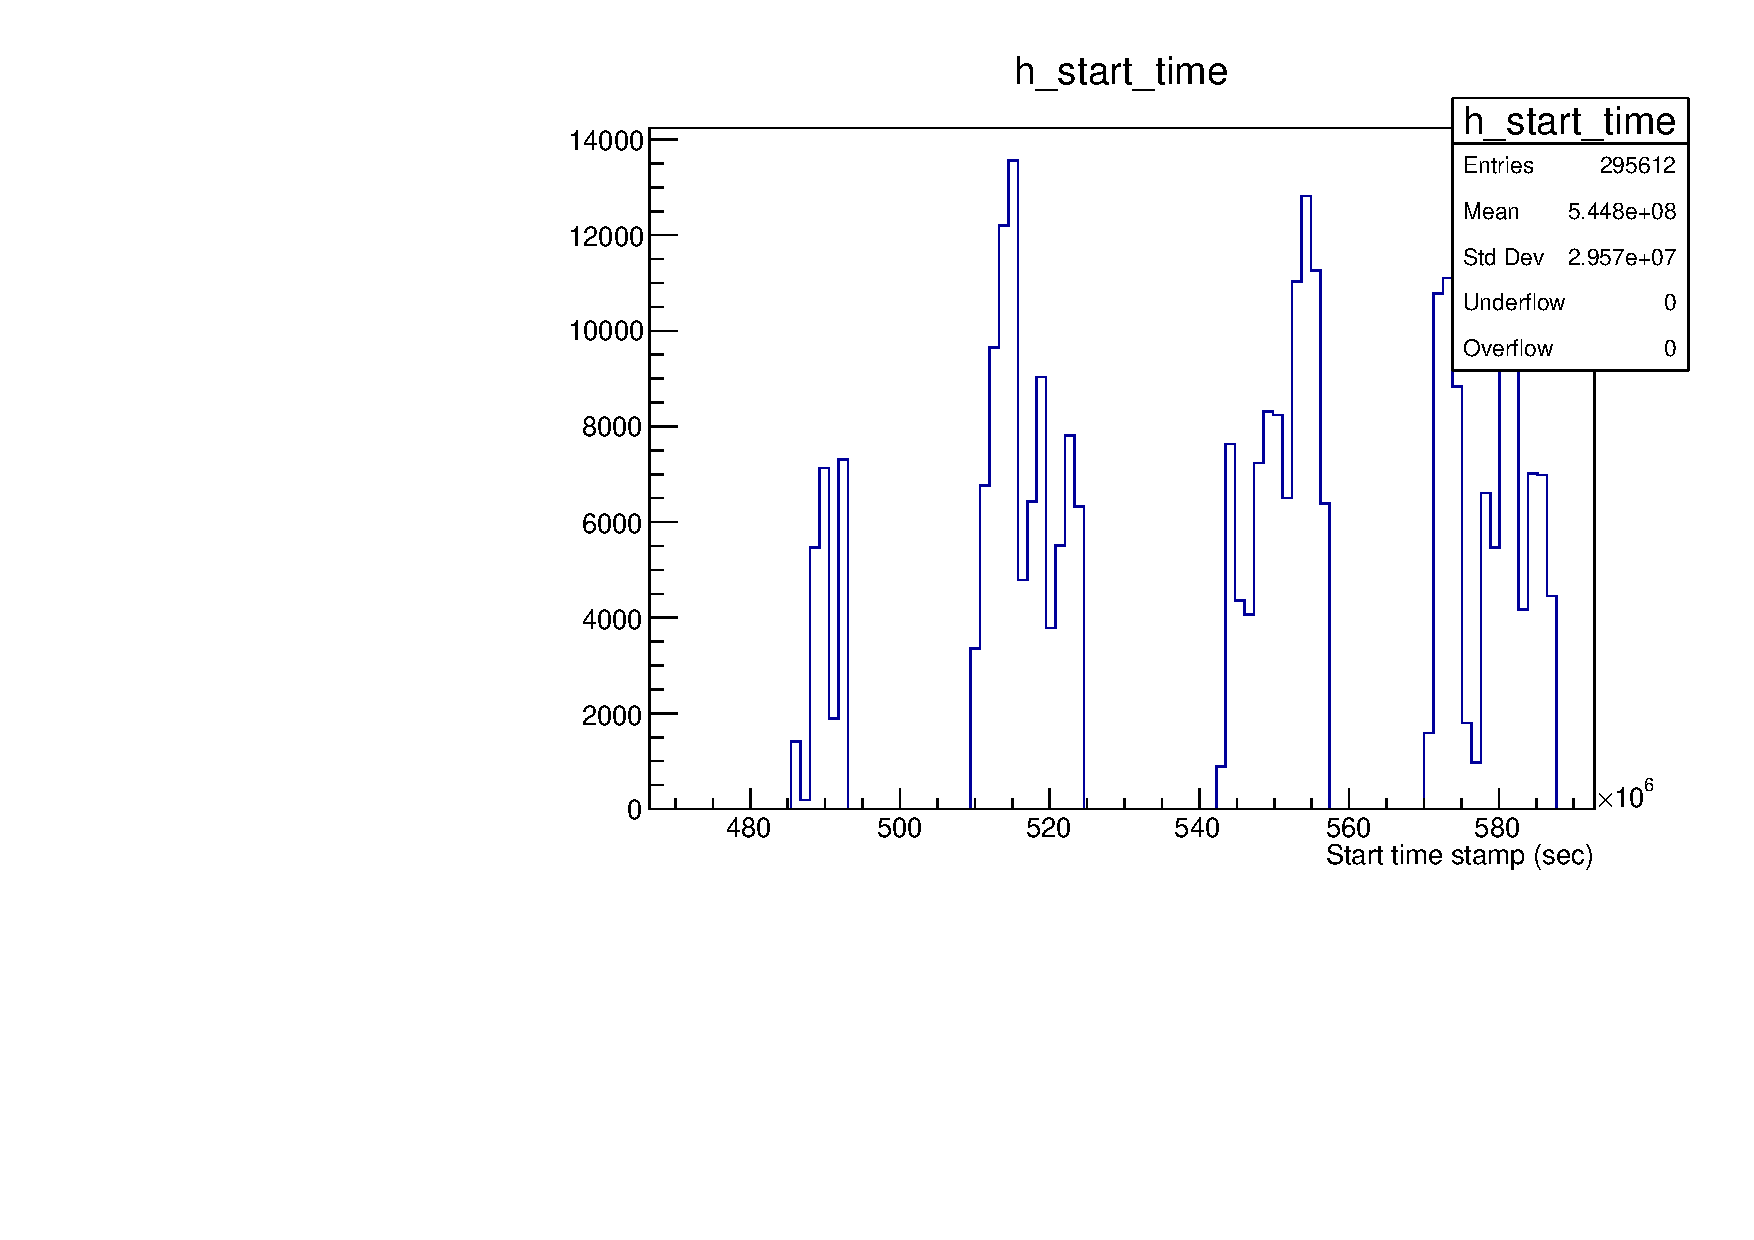
\includegraphics[width=0.4\textwidth]{figs/toy/fig_bin100_LIVxsec_0_random1_period1000_probe24_SigConfig0_LumiProf0_h_start_time.pdf}
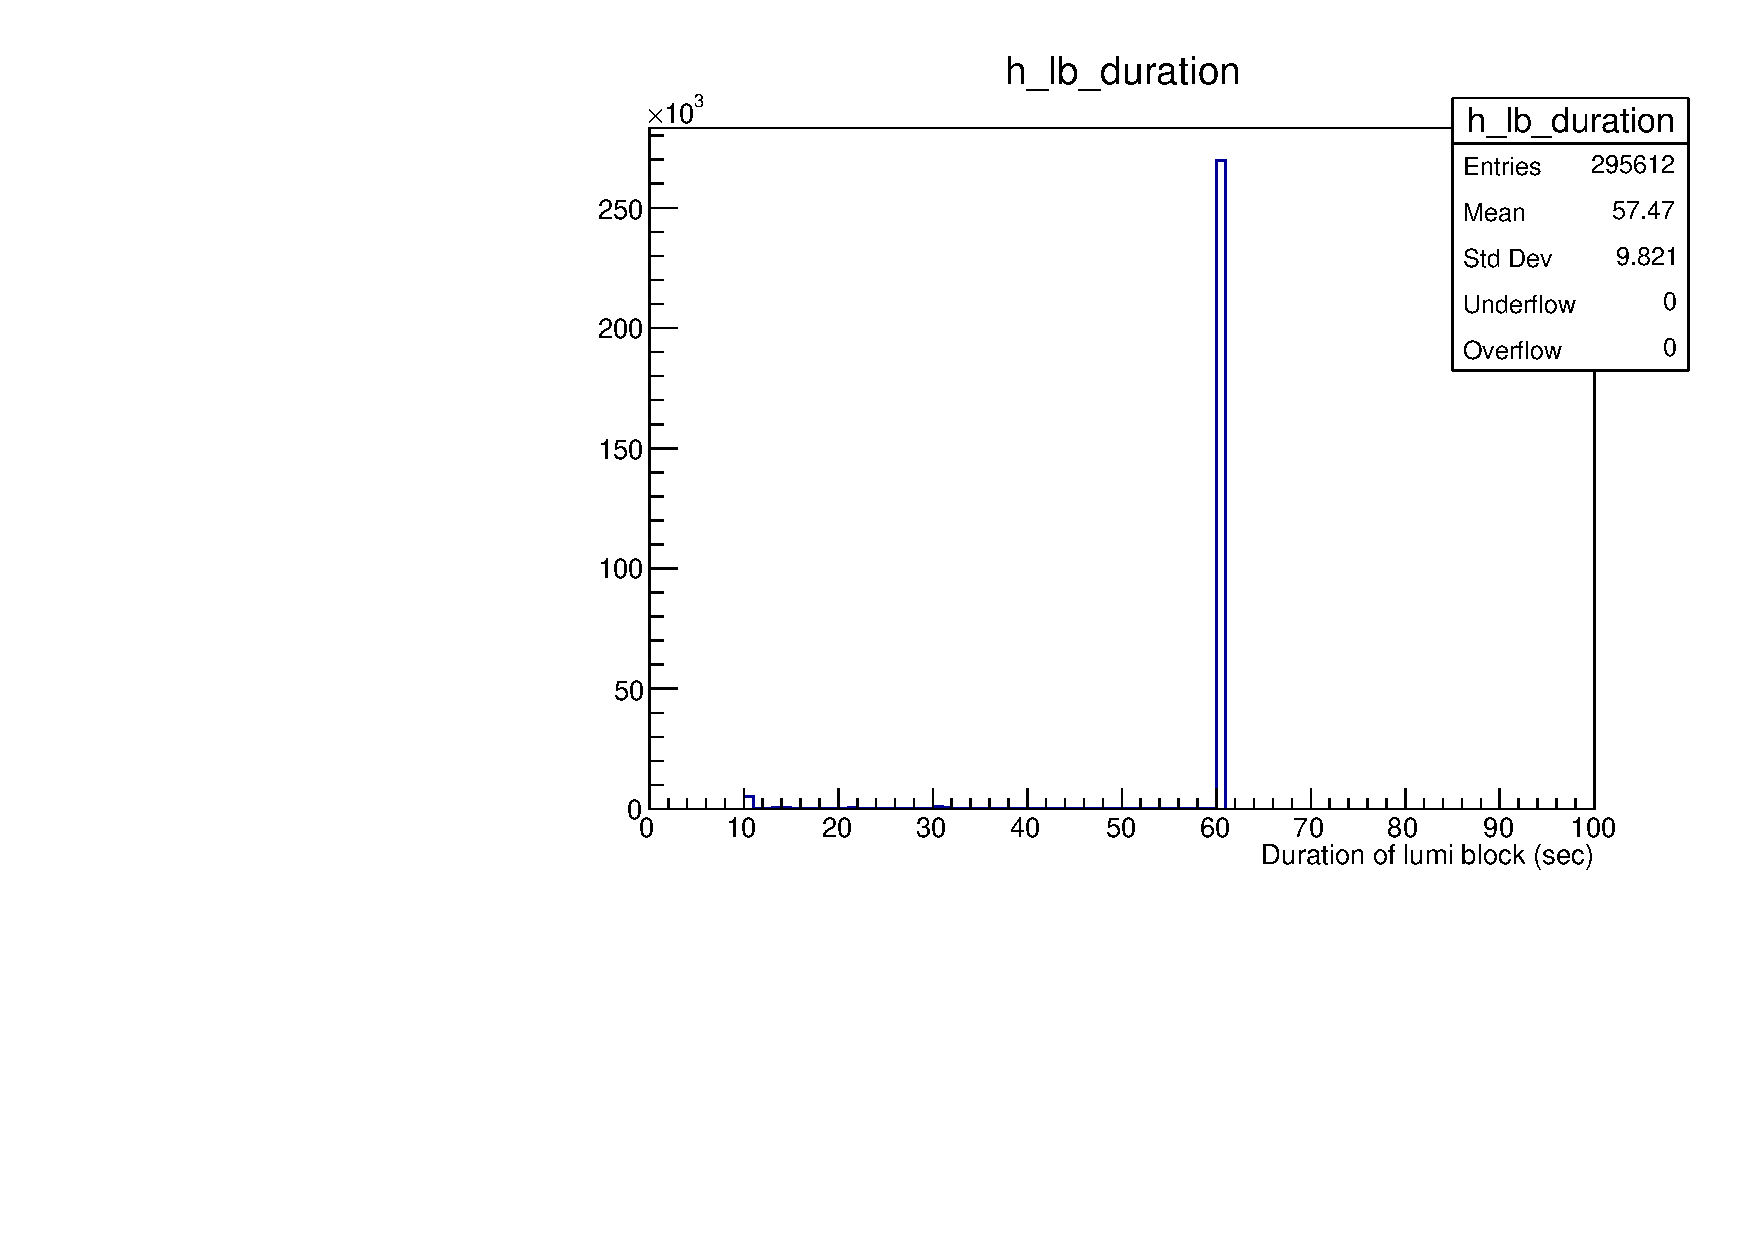
\includegraphics[width=0.4\textwidth]{figs/toy/fig_bin100_LIVxsec_0_random1_period1000_probe24_SigConfig0_LumiProf0_h_lb_duration.pdf}
\caption{\label{fig:toy_lumiProfile} Distribution of the time stamps of each Lumi block (left) and their duration (right). }
\end{figure}

As a basic TOY sample, the number of Z is computed each LB according to its duration and compute the Sidereal phase with following condition 
using only the time stamp of Lumi Block, and not use of other information in the actual data:
\begin{enumerate}
 \item use actual time stamp of each LB of Run-2 data.
 \item a Z fiducial cross sectin of 750 pb. (and inject LIV effect as function of sidereal phase if necessary)
 \item a flat instanteous luminosity of $1.0 \times 10^{34} cm^{-2} s^{-1}$ (as a simplest case). 
 \item introduce random effect on the computed number of Z by applying poisson statistics in each LB. 
 \item Siderial period, $T$, is 23h 56m 04s ($\sim$ 365 / 366 days). 
 \item $T_0$ is set March 20th 11:35 UTC, which is $T_0$ of SCF at the center of the ATLAS detector. (See Section~\ref{lab:Theory}).
\end{enumerate}

Histogram of number of LBs as function of the generated Sidereal period and sidereal phase are shown in Fig.~\ref{fig:toy_lb_period}.
These distributions are not flat because of run time (ATLAS is taking data when LHC makes collision when ATLAS detector is ready.) 
Distribution of the integrated luminosity as a function of sidereal phase and number of Z boson are shown in Fig.~\ref{fig:toy_numZ_phase}. 
Non-uniform structure of this distribution is due to the non-uniform profile of time stamp of the lumi blocks.
For example, a fill in 2018 started at 8:00 and lasted 7 hours and no other fill on the same day. In this case, 
we have measured the number of Z only 7 hours over 24 hours. 

\begin{figure}
\centering
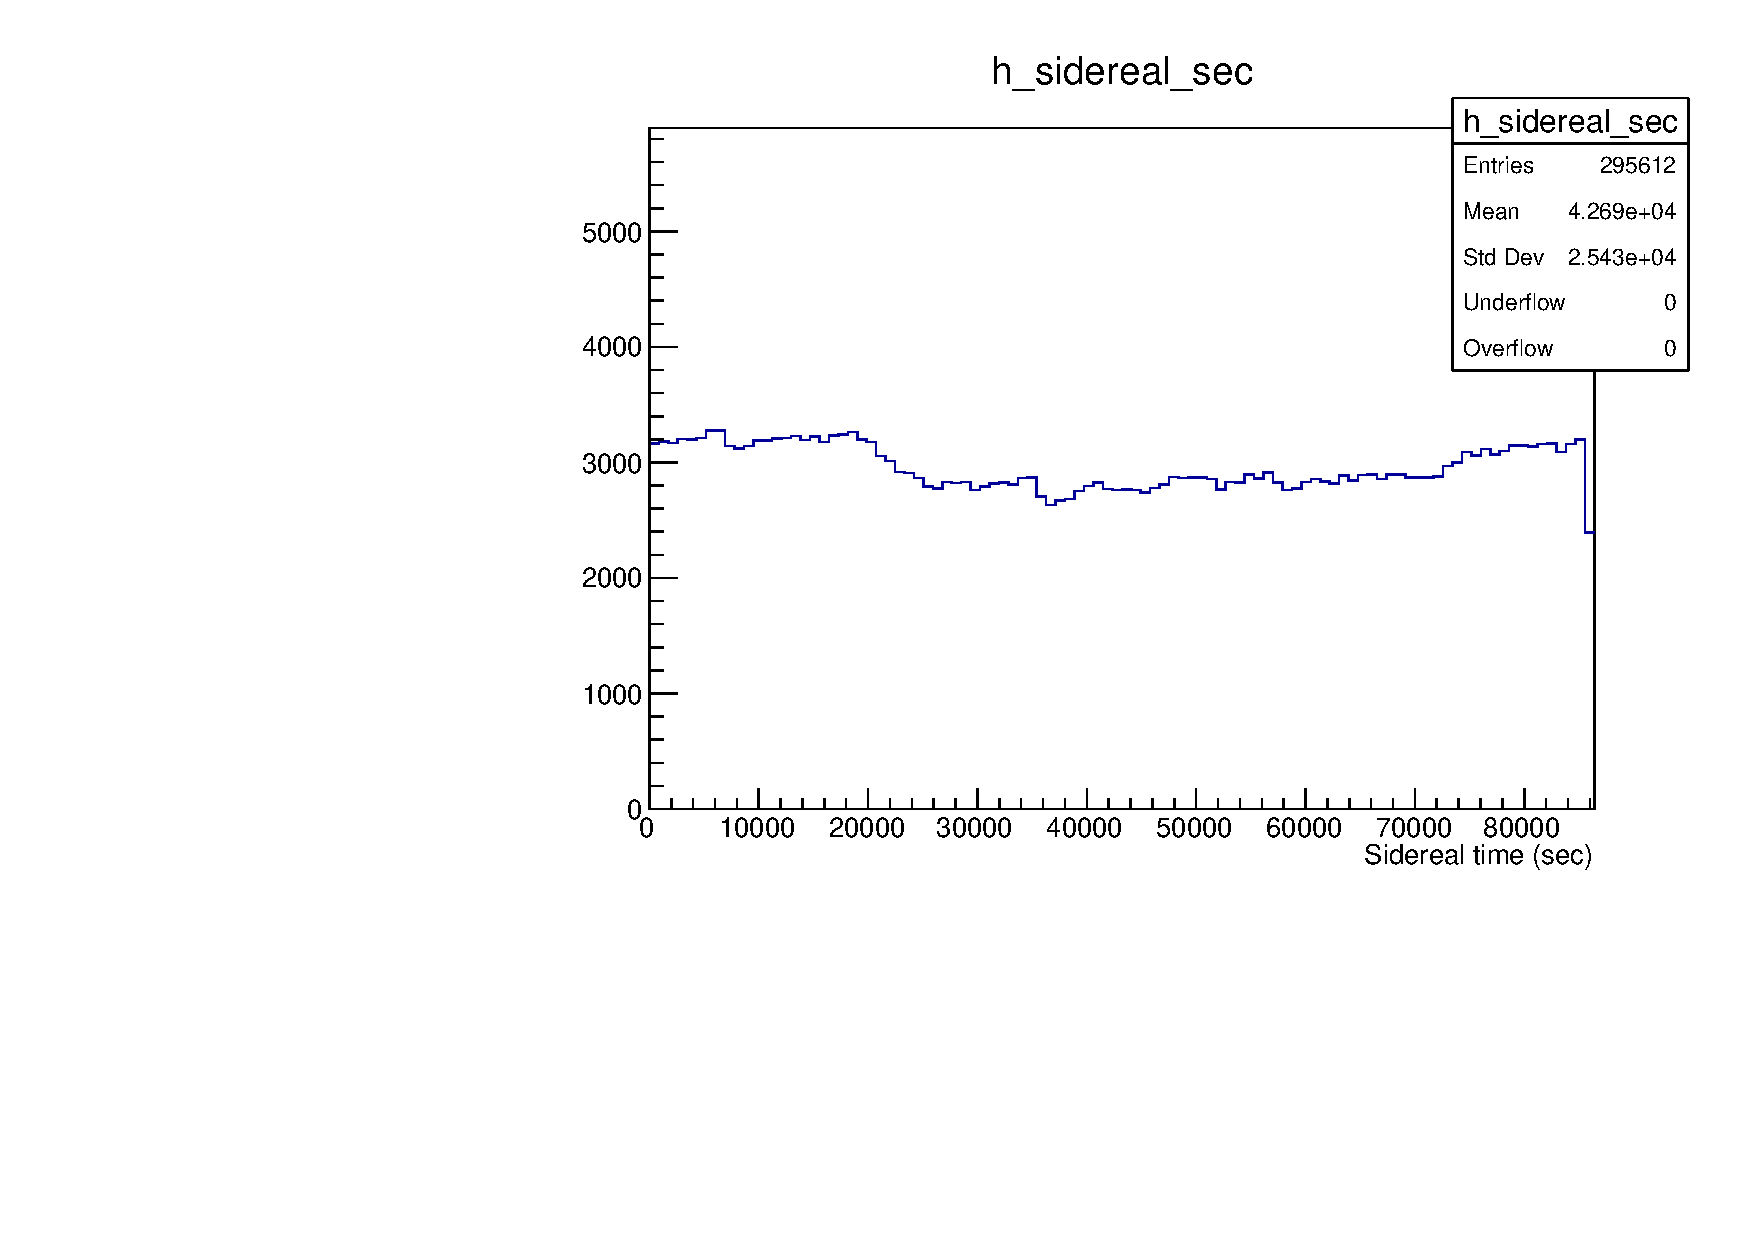
\includegraphics[width=0.4\textwidth]{figs/toy/fig_bin100_LIVxsec_0_random1_period1000_probe24_SigConfig0_LumiProf0_h_sidereal_sec.pdf}
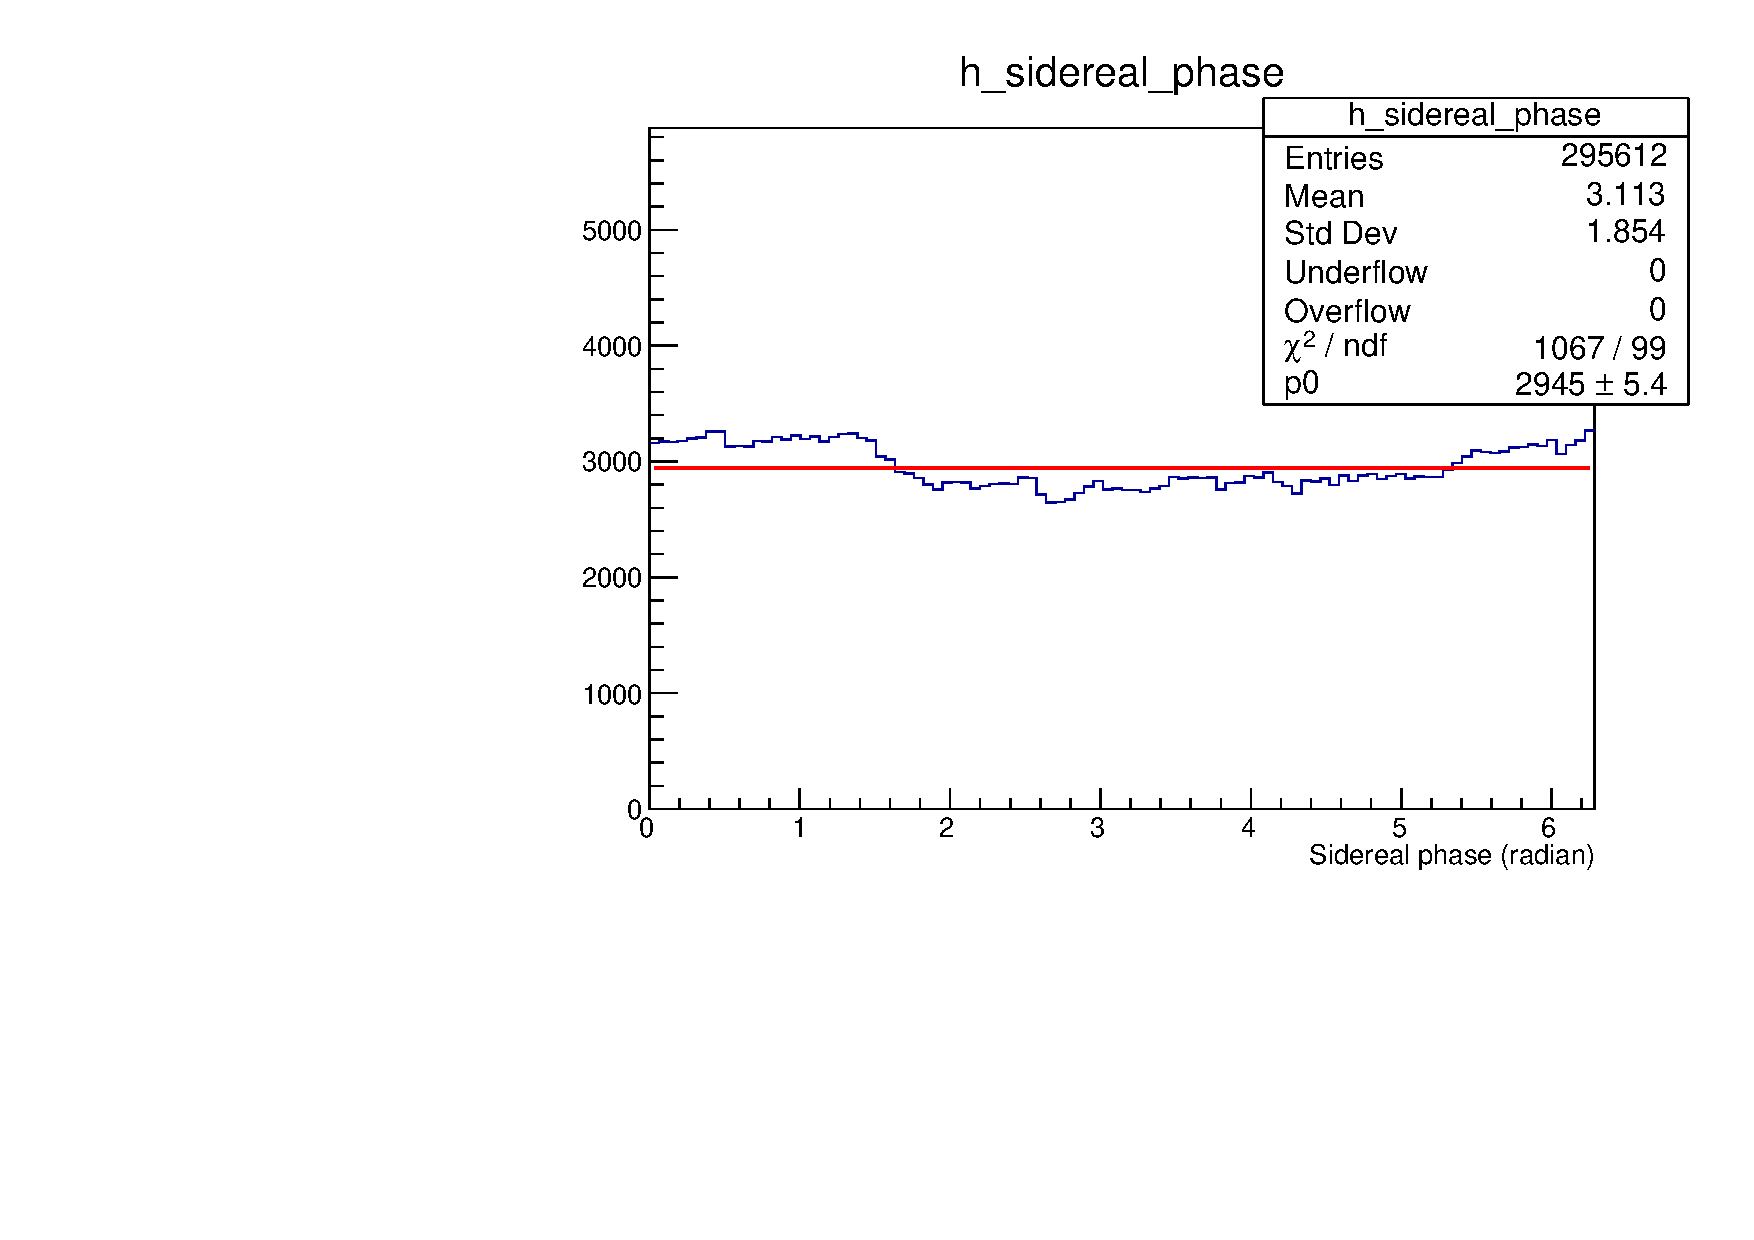
\includegraphics[width=0.4\textwidth]{figs/toy/fig_bin100_LIVxsec_0_random1_period1000_probe24_SigConfig0_LumiProf0_h_sidereal_phase.pdf}
\caption{\label{fig:toy_lb_period} Distribution of Lumi block as function of the sidereal period (left) and the sidereal phase (right). }
\end{figure}

\begin{figure}
\centering
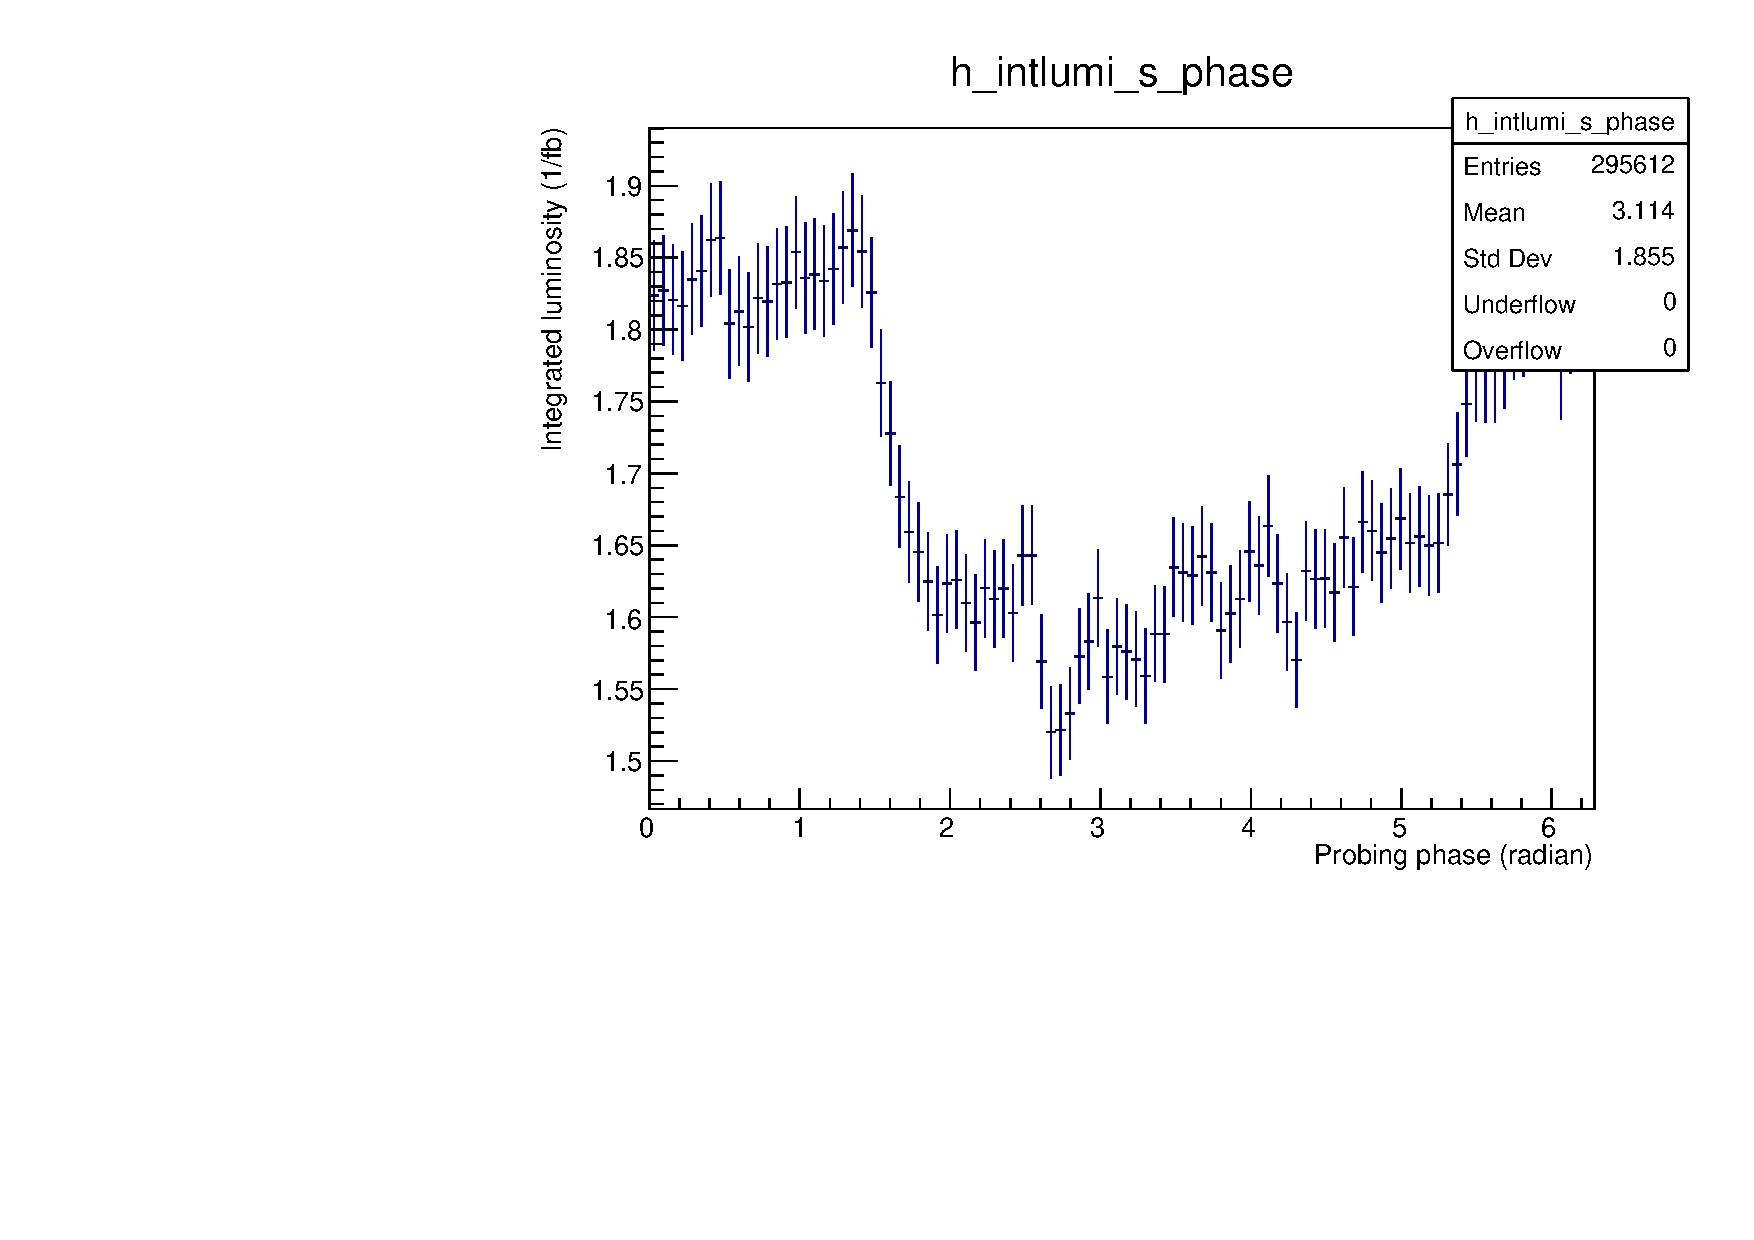
\includegraphics[width=0.4\textwidth]{figs/toy/fig_bin100_LIVxsec_0_random1_period1000_probe24_SigConfig0_LumiProf0_h_intlumi_s_phase.pdf}
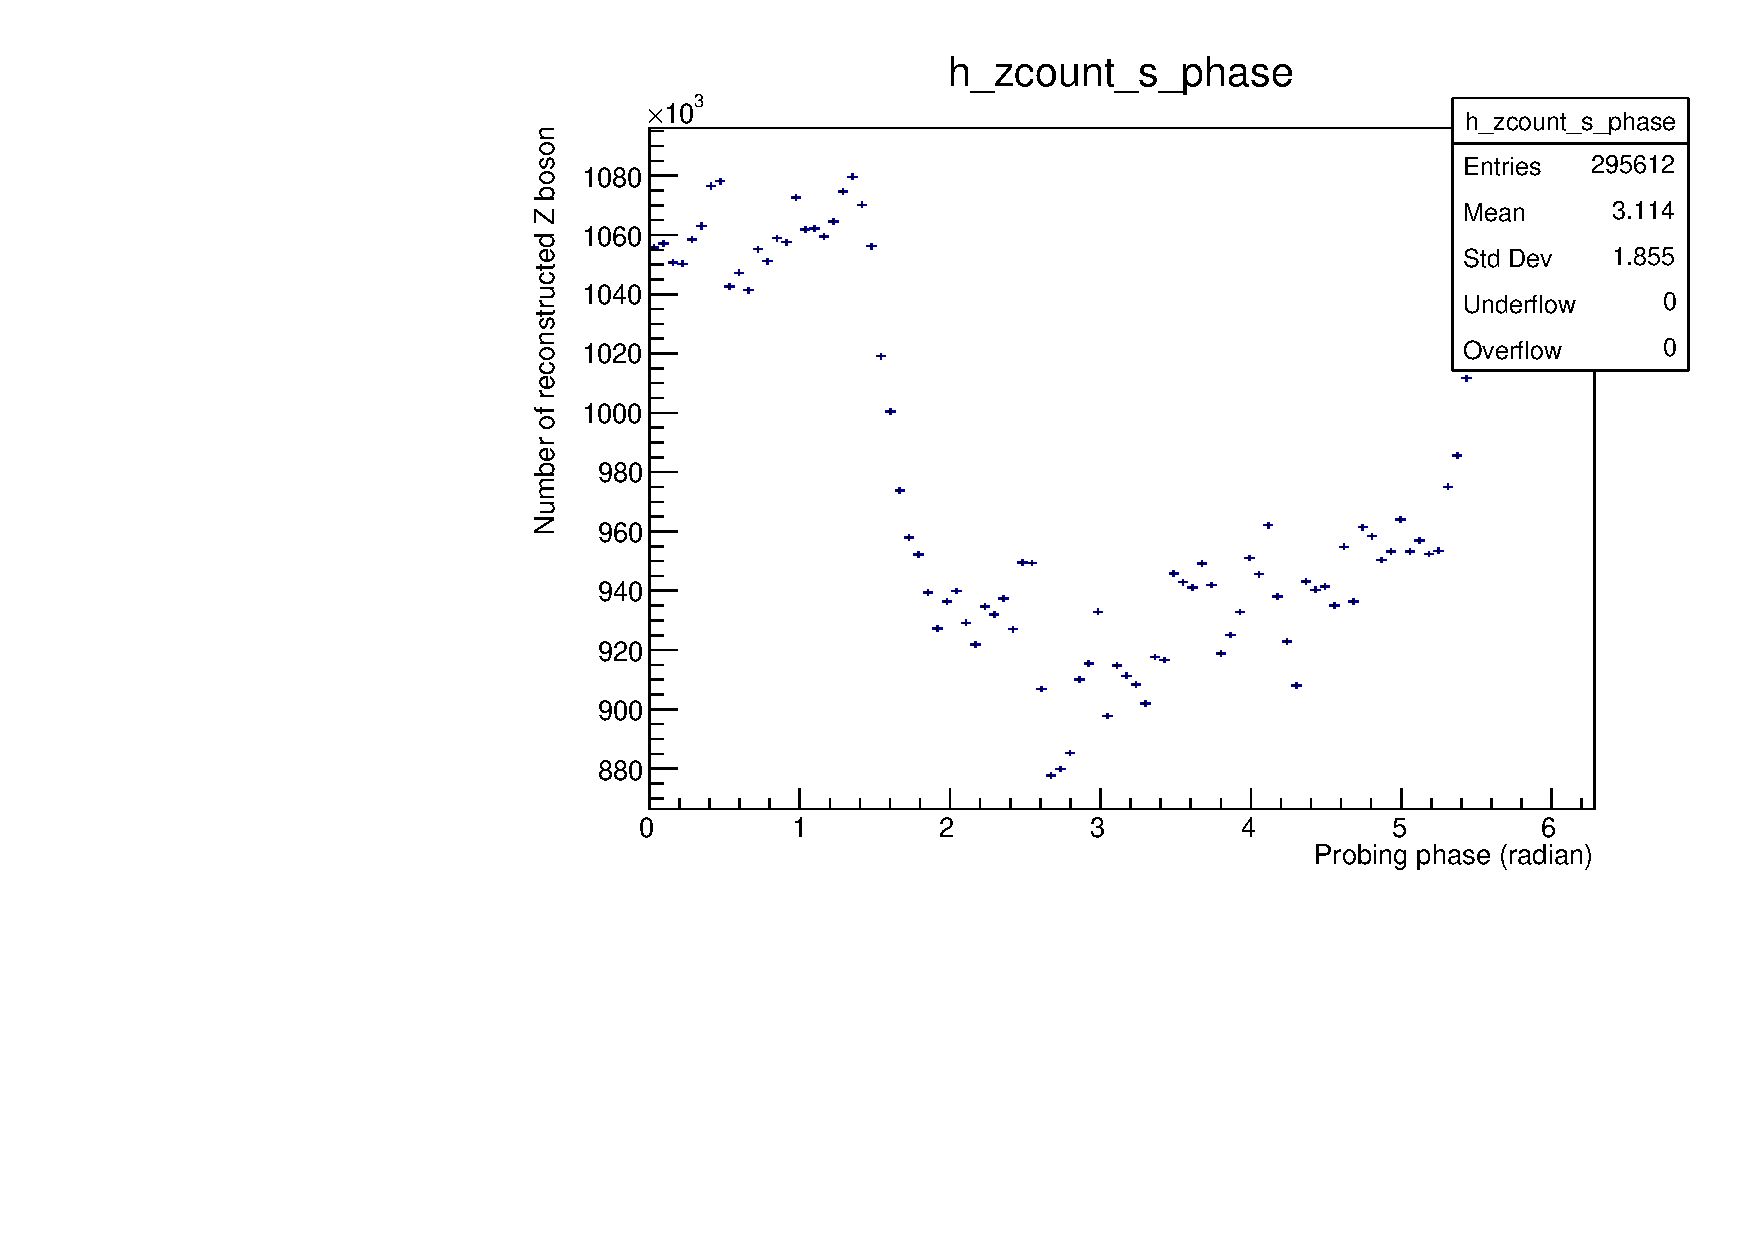
\includegraphics[width=0.4\textwidth]{figs/toy/fig_bin100_LIVxsec_0_random1_period1000_probe24_SigConfig0_LumiProf0_h_zcount_s_phase.pdf}
\caption{\label{fig:toy_numZ_phase} Integrated Lumiminoisty (left) and number of Z boson (right) for each sidereal phase bin (100 bins over 2$\pi$.) }
\end{figure}

In order to probe tiny effect, we take the double ratio as Eq.~\ref{eq:double_ratio}. 
The distribution of the double ratio is shown in Fig.~\ref{fig:toy_Dratio_phase}. 
On this TOY configuration, $\mathcal{L}_{int} = 178.2 fb^{-1}$, because we assume a flat instanteneous luminosity.

\begin{figure}
\centering
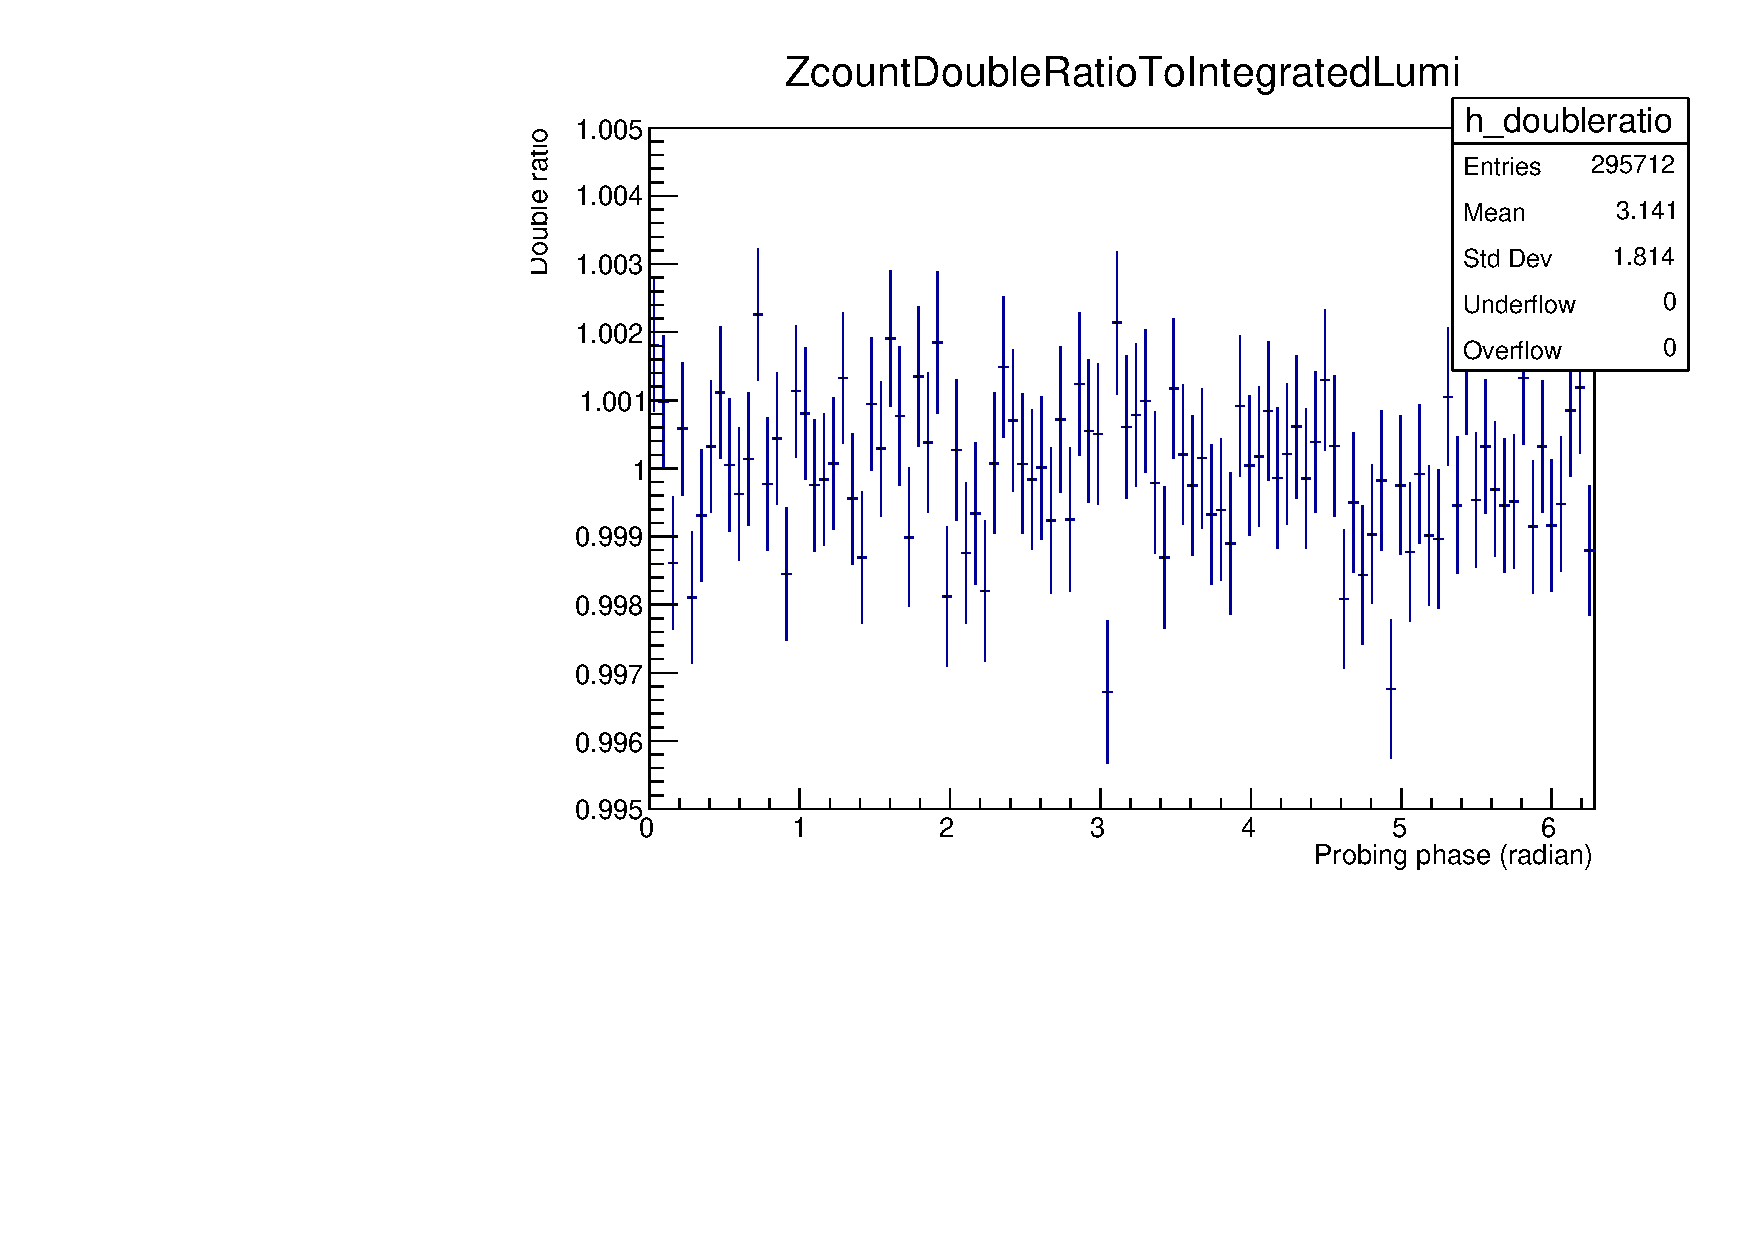
\includegraphics[width=0.4\textwidth]{figs/toy/fig_bin100_LIVxsec_0_random1_period1000_probe24_SigConfig0_LumiProf0_ZcountDoubleRatioToIntegratedLumi.pdf}
\caption{\label{fig:toy_Dratio_phase} The Double ratio for each sidereal phase bin (100 bins over 2$\pi$.) }
\end{figure}

Statistical uncertainties are shown in the error bar in Fig.~\ref{fig:toy_Dratio_phase}. In Figs.~\ref{fig:toy_Dratio_proj}, the projection of the double ratio and
 it's pull are shown. The mean and RMS of the pull distribution are consistent with 1.0, which shows reasonable error propagation has been made. 

\begin{figure}
\centering
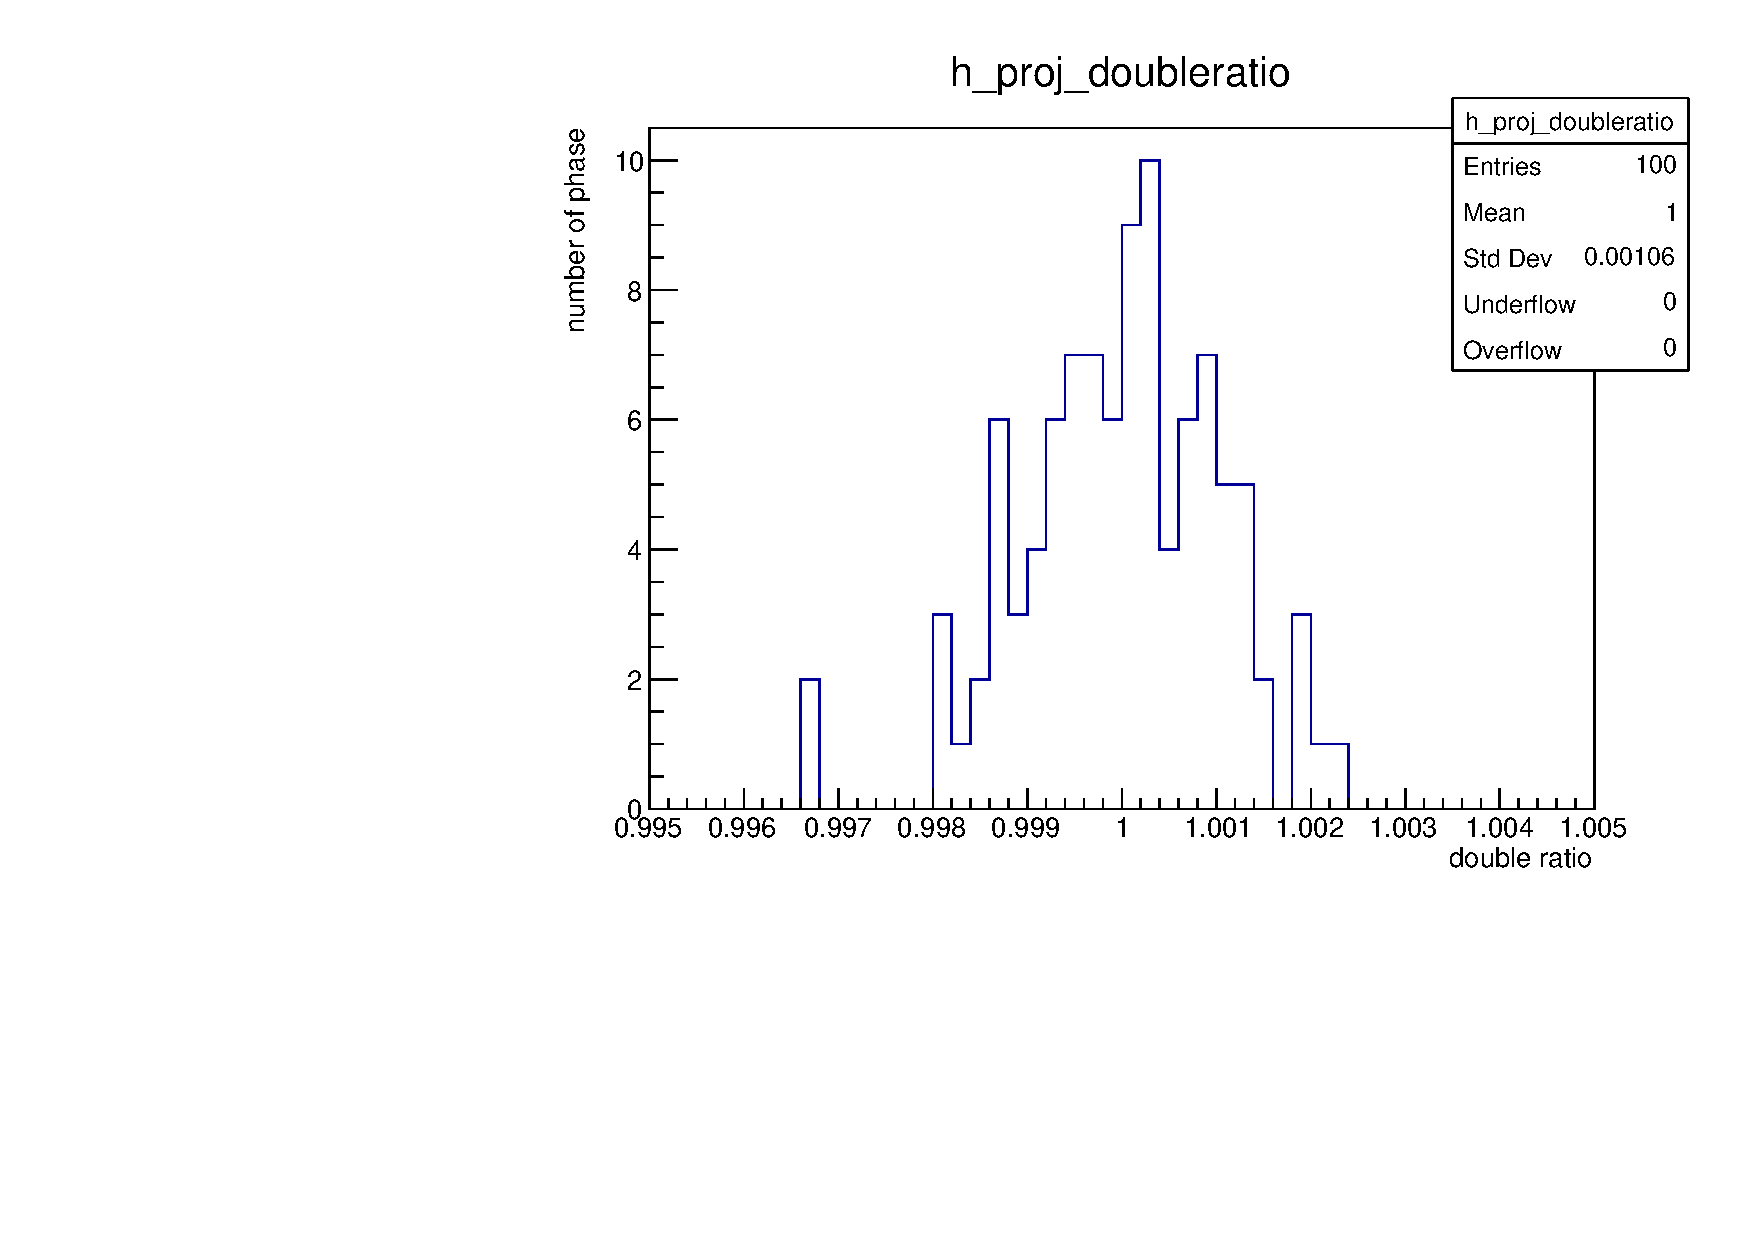
\includegraphics[width=0.4\textwidth]{figs/toy/fig_bin100_LIVxsec_0_random1_period1000_probe24_SigConfig0_LumiProf0_h_proj_doubleratio.pdf}
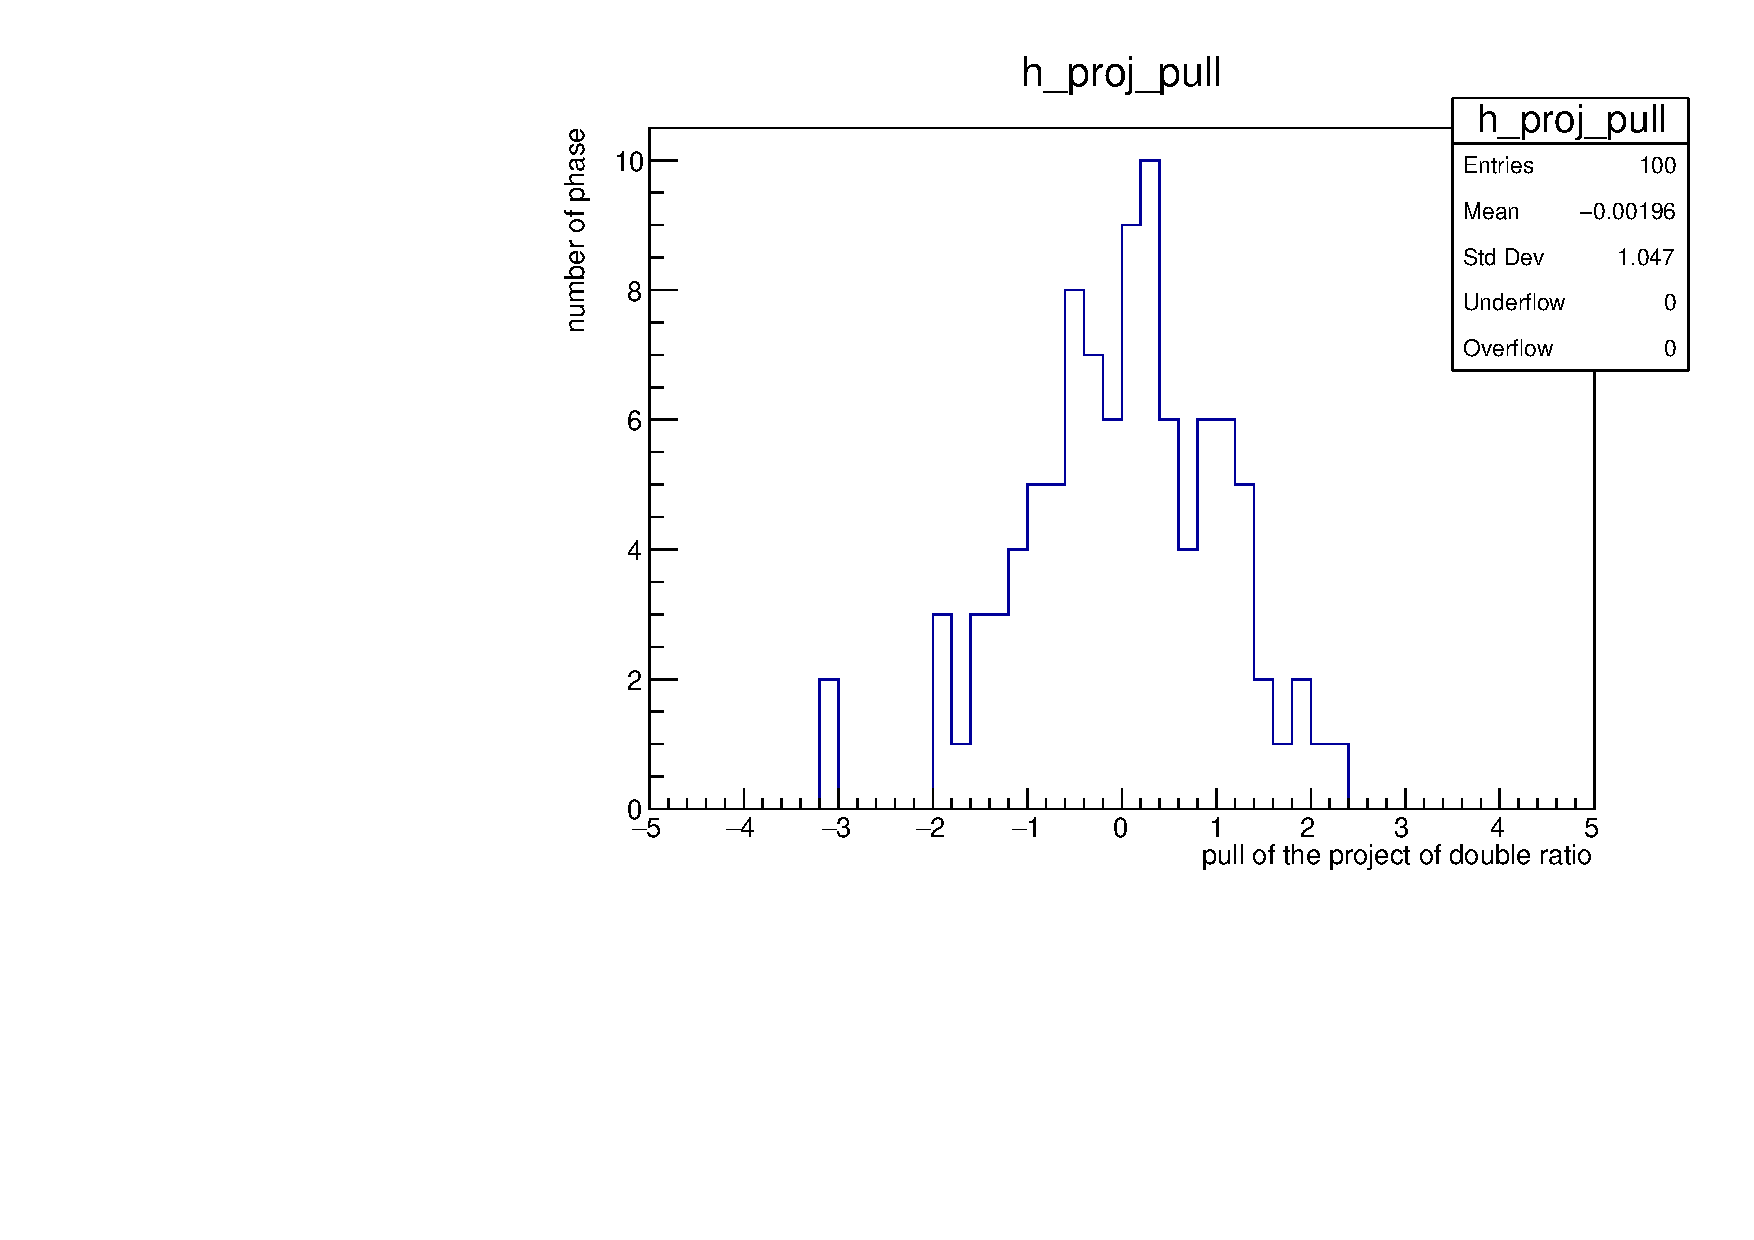
\includegraphics[width=0.4\textwidth]{figs/toy/fig_bin100_LIVxsec_0_random1_period1000_probe24_SigConfig0_LumiProf0_h_proj_pull.pdf}
\caption{\label{fig:toy_Dratio_proj} Projection of Fig.~\ref{fig:toy_Dratio_phase} (left) and pull distribution. }
\end{figure}



%% 
%% 
%% There are three types of TOY sample. 
%% \begin{enumerate}
%% \item[i] simplest: flat instanteneous luminosity (1.0 x $10^{34} cm^{-2}s^{-1}$) with time stamp of data lumi block.
%% \item[ii] data profile: data luminosity profile with with time stamp of data lumi block.
%% \item[iii] realistic: introduce additional efficiency degradation effect in addtion to (ii)
%% \end{enumerate}
%% 

%% \subsection{How the sidereal effect look like}

Figures ~\ref{fig:toy_Dratio_phase_s1pb} show the double ratio in case of LIV signal amplitude of 1 pb with sin wave. 
Just for illustration purpose, prepared with and without statistics fluctuation. 
The amplitude of no randome case is around 0.00133, which is from the cross section ratio of 1 pb over 750 pb, which is used to generate this Toy experiment.

\begin{figure}
\centering
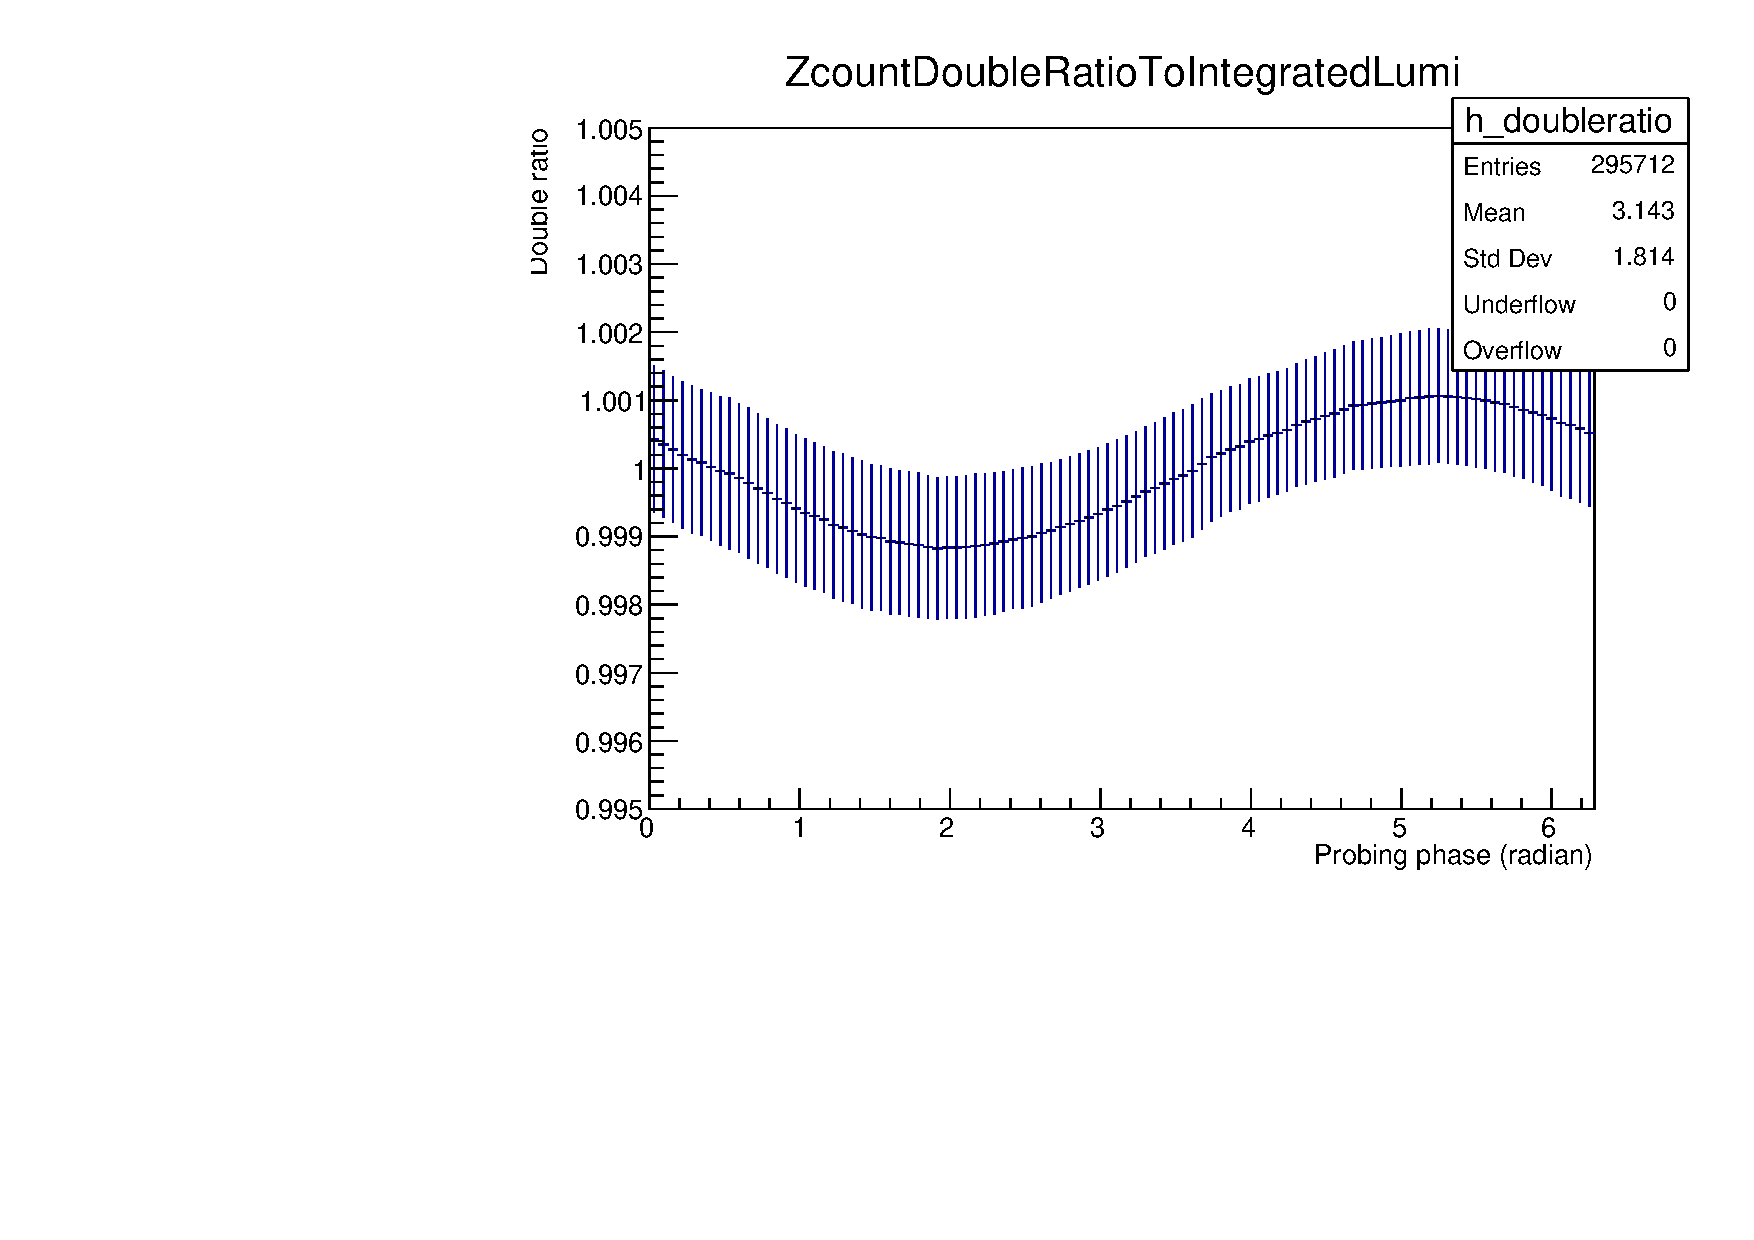
\includegraphics[width=0.4\textwidth]{figs/toy/fig_bin100_LIVxsec_1000_random0_period1000_probe24_SigConfig20_LumiProf0_ZcountDoubleRatioToIntegratedLumi.pdf}
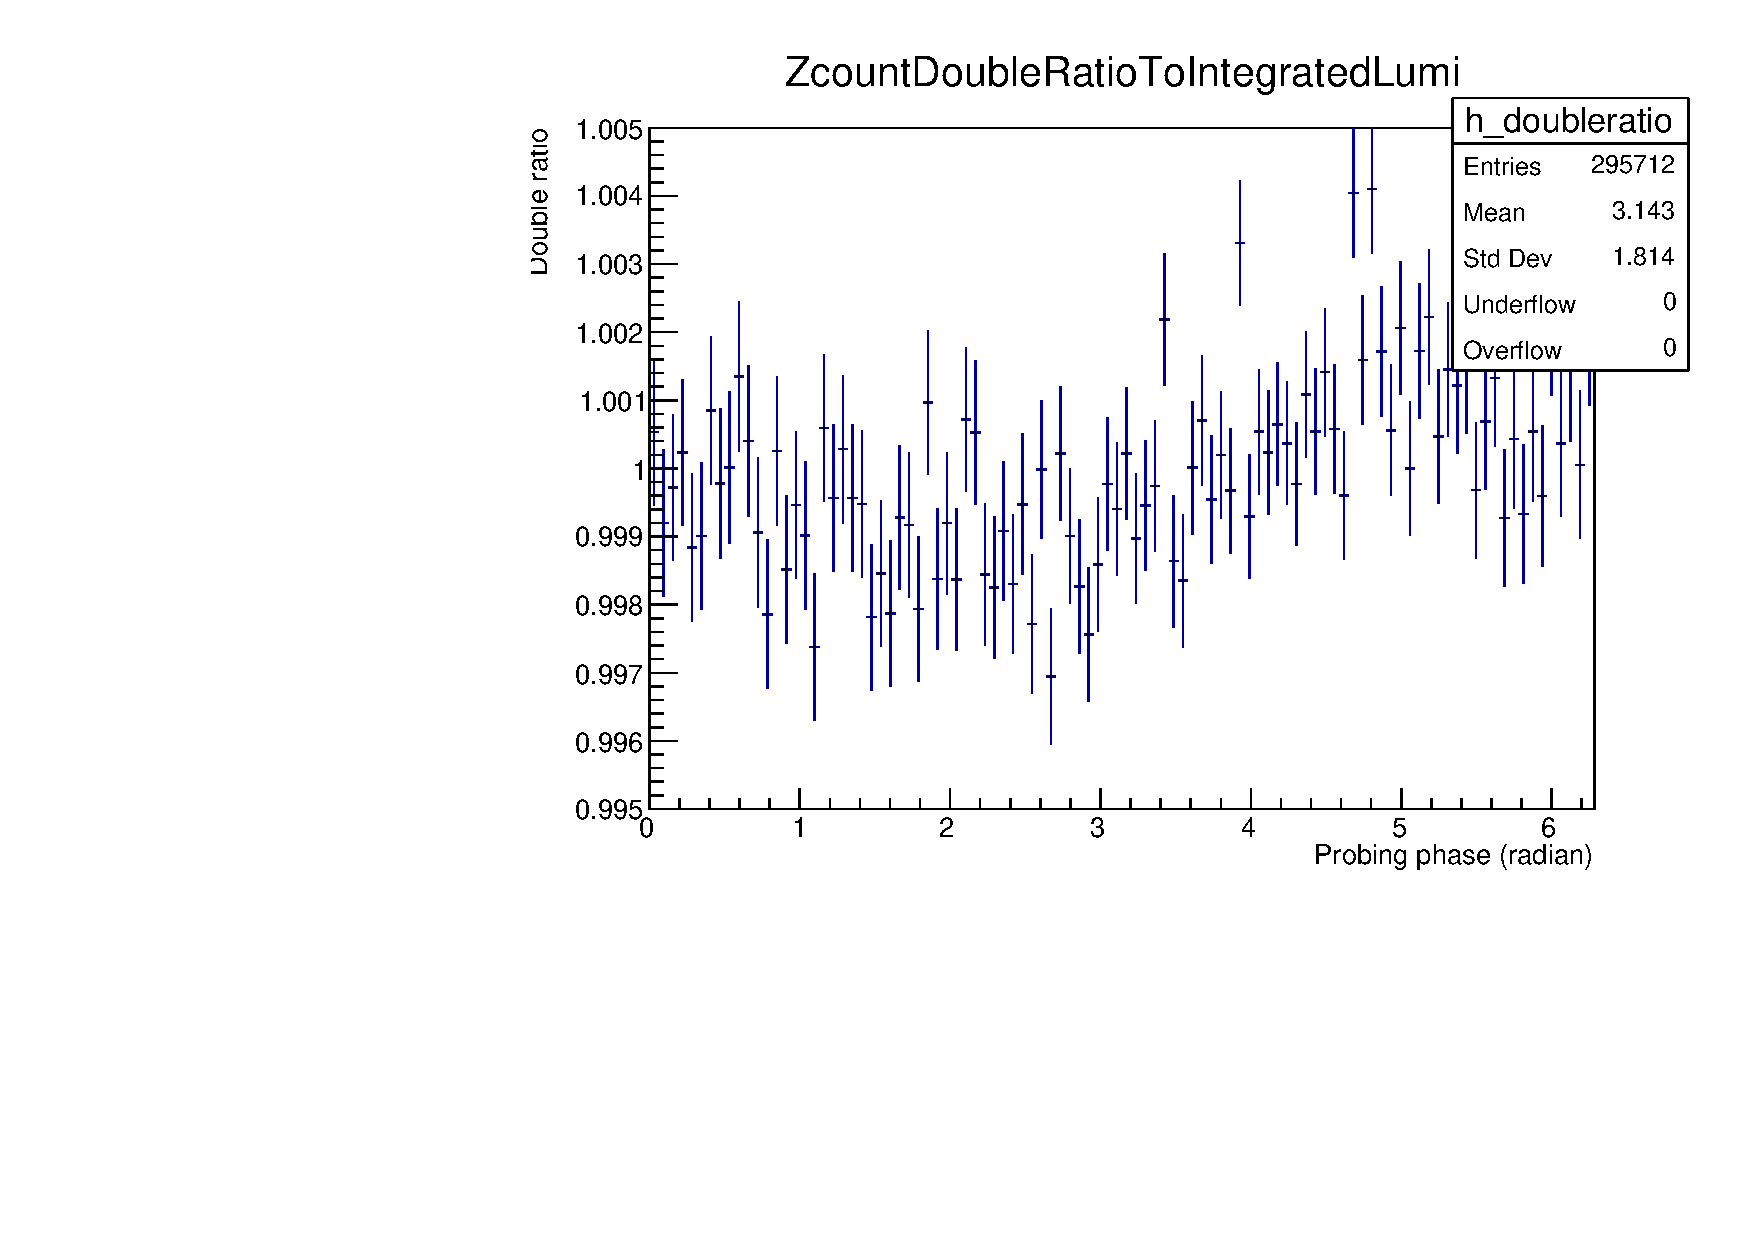
\includegraphics[width=0.4\textwidth]{figs/toy/fig_bin100_LIVxsec_1000_random1_period1000_probe24_SigConfig20_LumiProf0_ZcountDoubleRatioToIntegratedLumi.pdf}
\caption{\label{fig:toy_Dratio_phase_s1pb} The double ratio for each sidereal phase bin (100 bins over 2$\pi$.) with LIV signal amplitude of 1 pb. }
\end{figure}


\subsection{Study with TOY data}

 By using Toy data, some basic studies are performed. 

\subsubsection{No signal case}

 This is test on NULL signal hypothesis. Figure~\ref{fig:toy_Dratio_phase_null} shows the double ratio with NULL signal, for both with and without statistical fluctuation.
Based on this configuration, 1000 Toy experiments are generated and fit simple sin and cosin curve. The results of these fit are shown in Fig.~\ref{fig:toy_1000exp_s0pb}. 
Mean value are consistent with zero, and the RMS is 0.00012. From this, we have statistical limit around 10 to -4. 

\begin{figure}
\centering
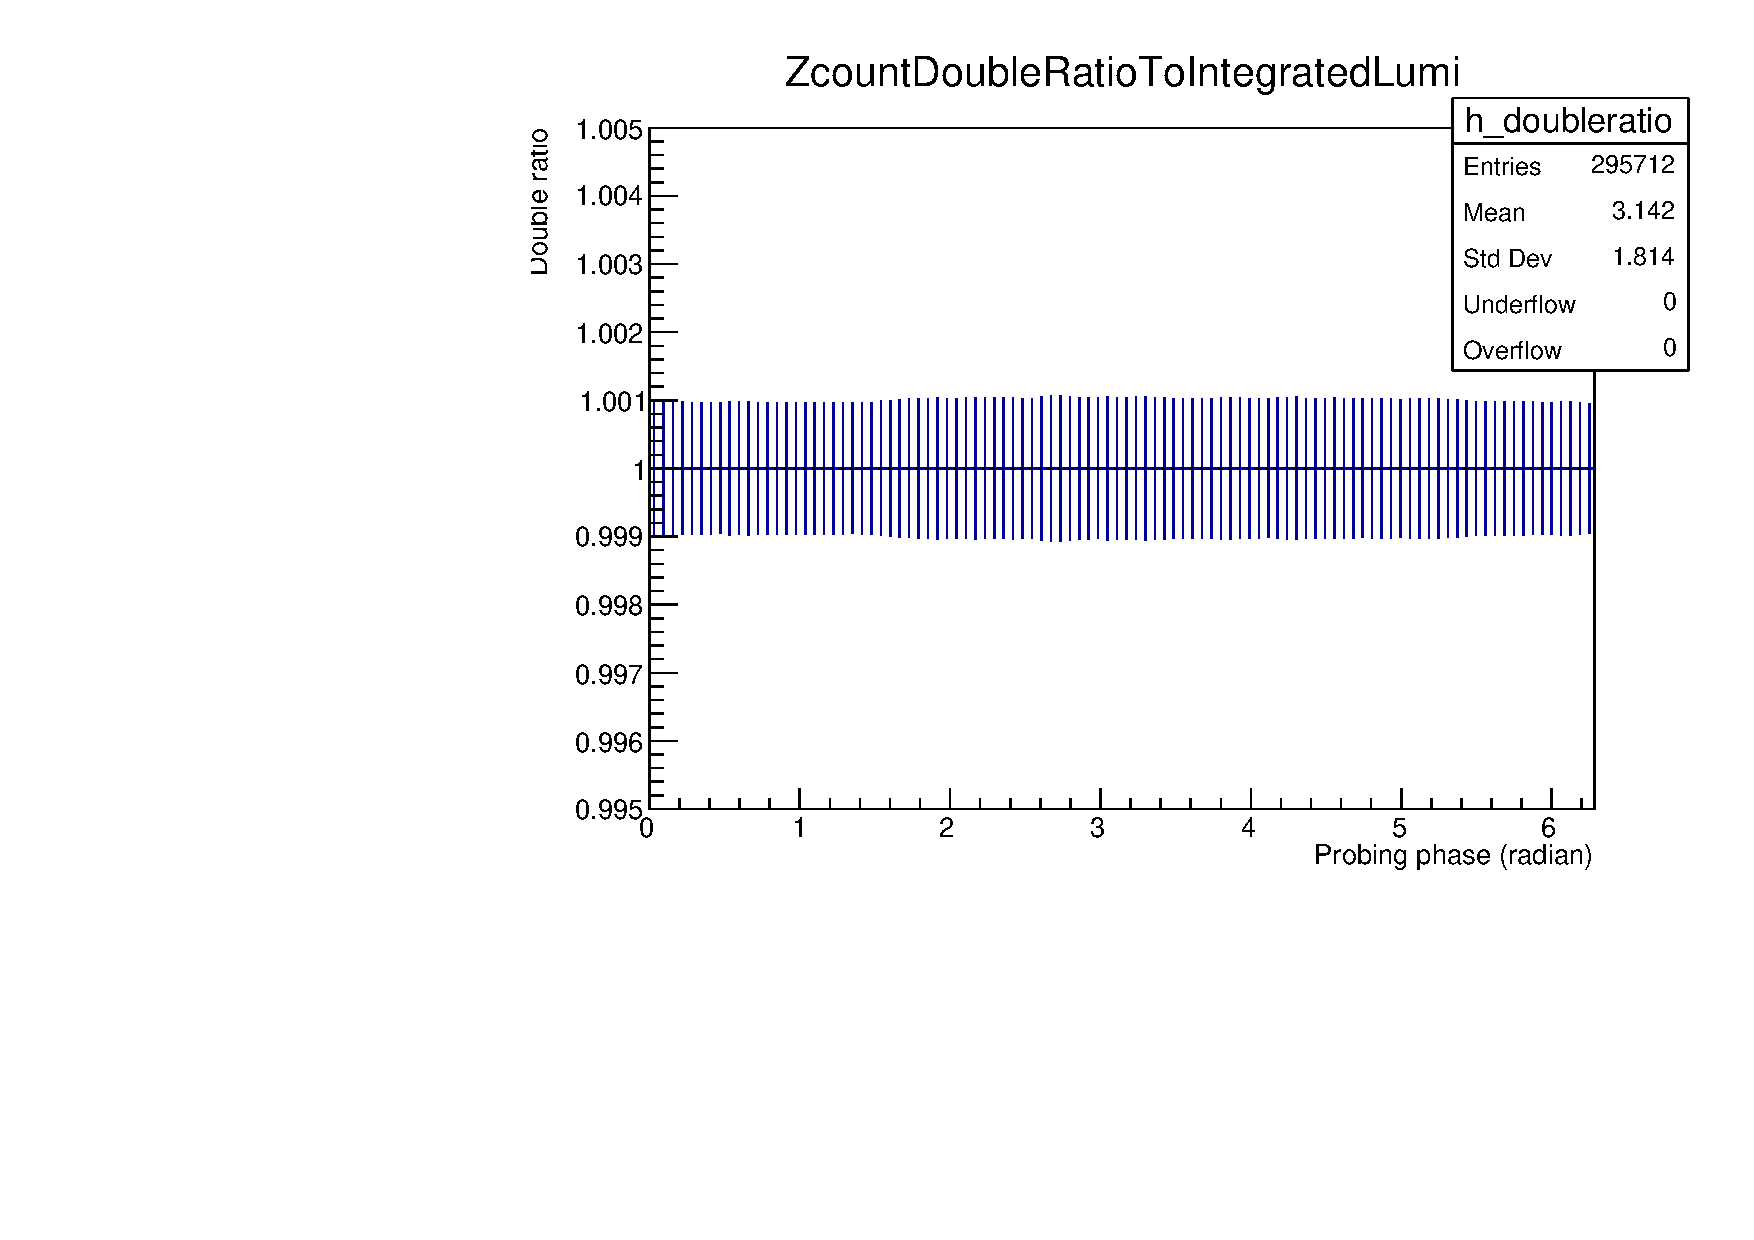
\includegraphics[width=0.4\textwidth]{figs/toy/fig_bin100_LIVxsec_0_random0_period1000_probe24_SigConfig0_LumiProf0_ZcountDoubleRatioToIntegratedLumi.pdf}
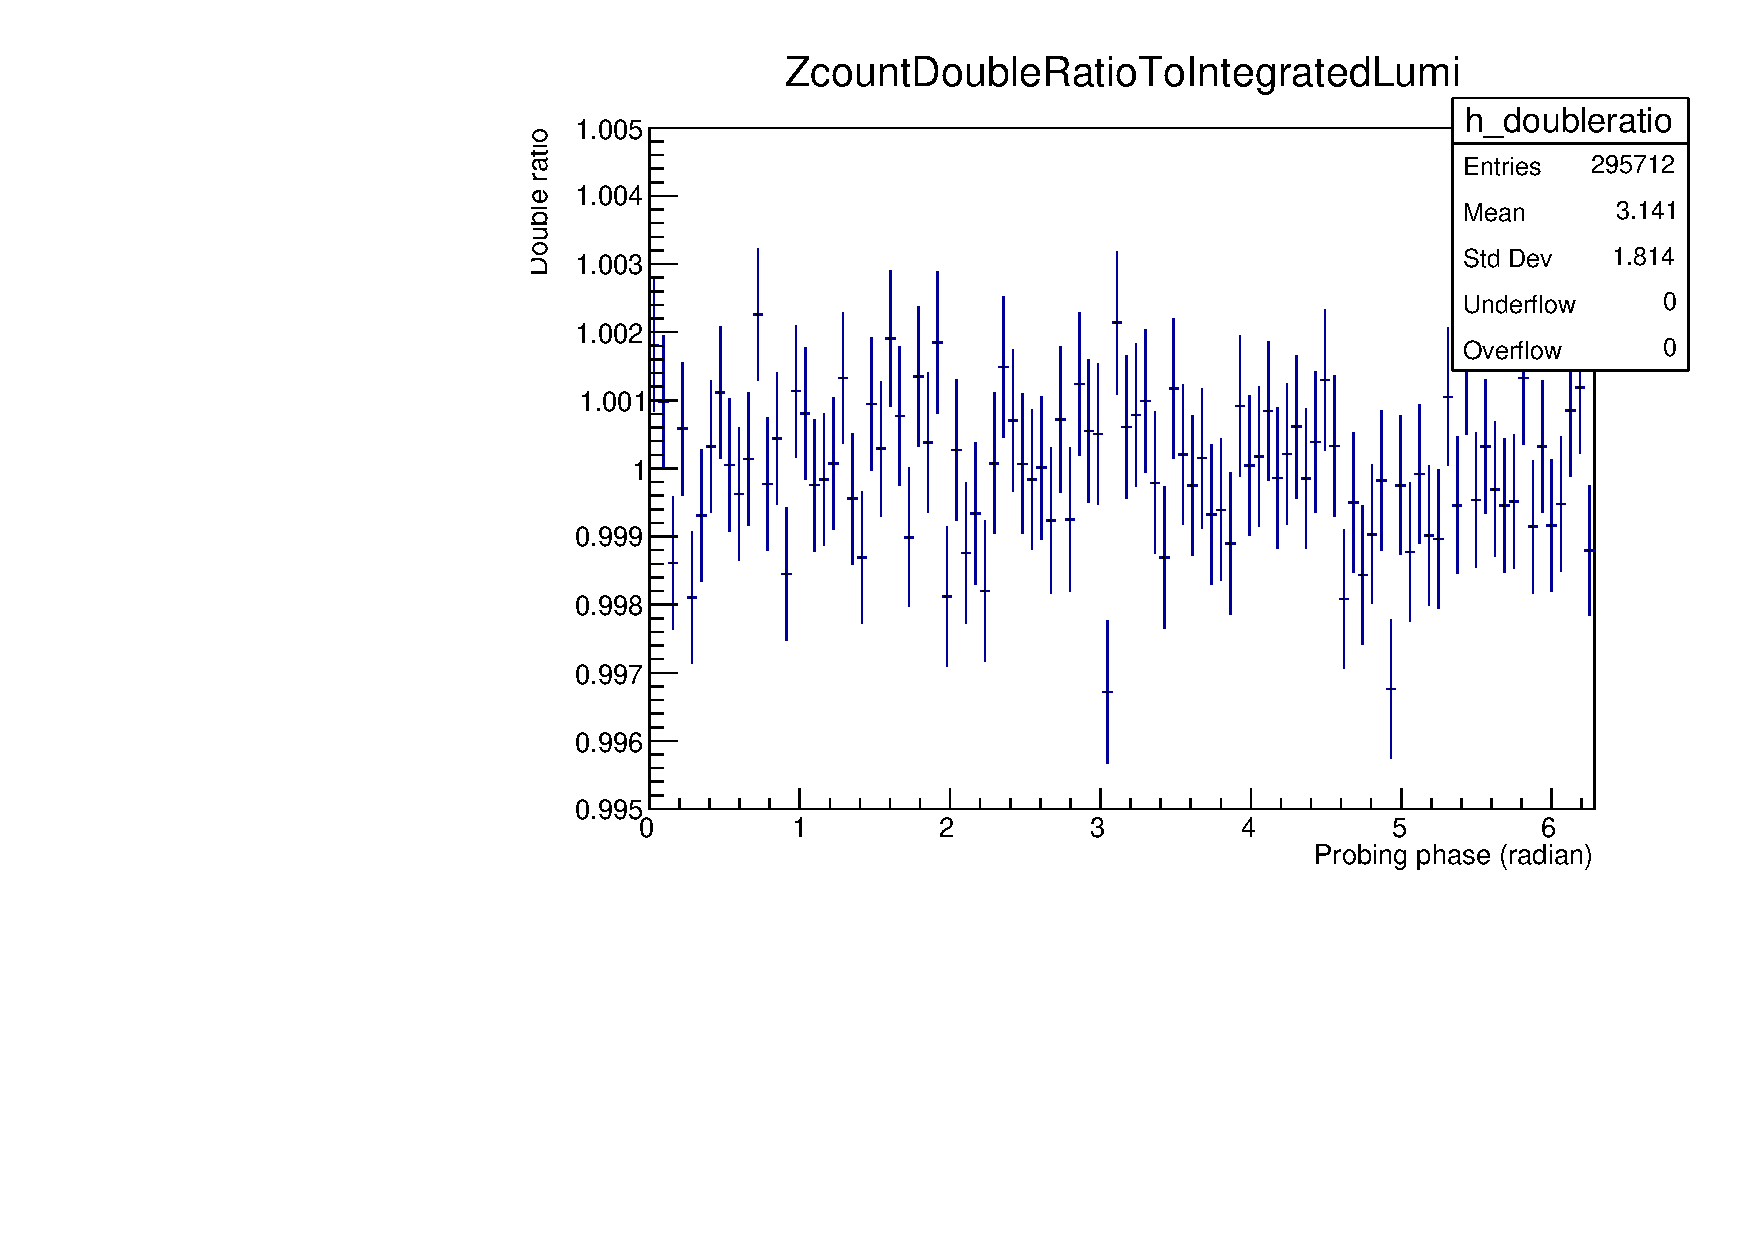
\includegraphics[width=0.4\textwidth]{figs/toy/fig_bin100_LIVxsec_0_random1_period1000_probe24_SigConfig0_LumiProf0_ZcountDoubleRatioToIntegratedLumi.pdf}
\caption{\label{fig:toy_Dratio_phase_null} The double ratio for each sidereal phase bin (100 bins over 2$\pi$.) with LIV signal amplitude of 0 pb (NULL signal). }
\end{figure}


\begin{figure}
\centering
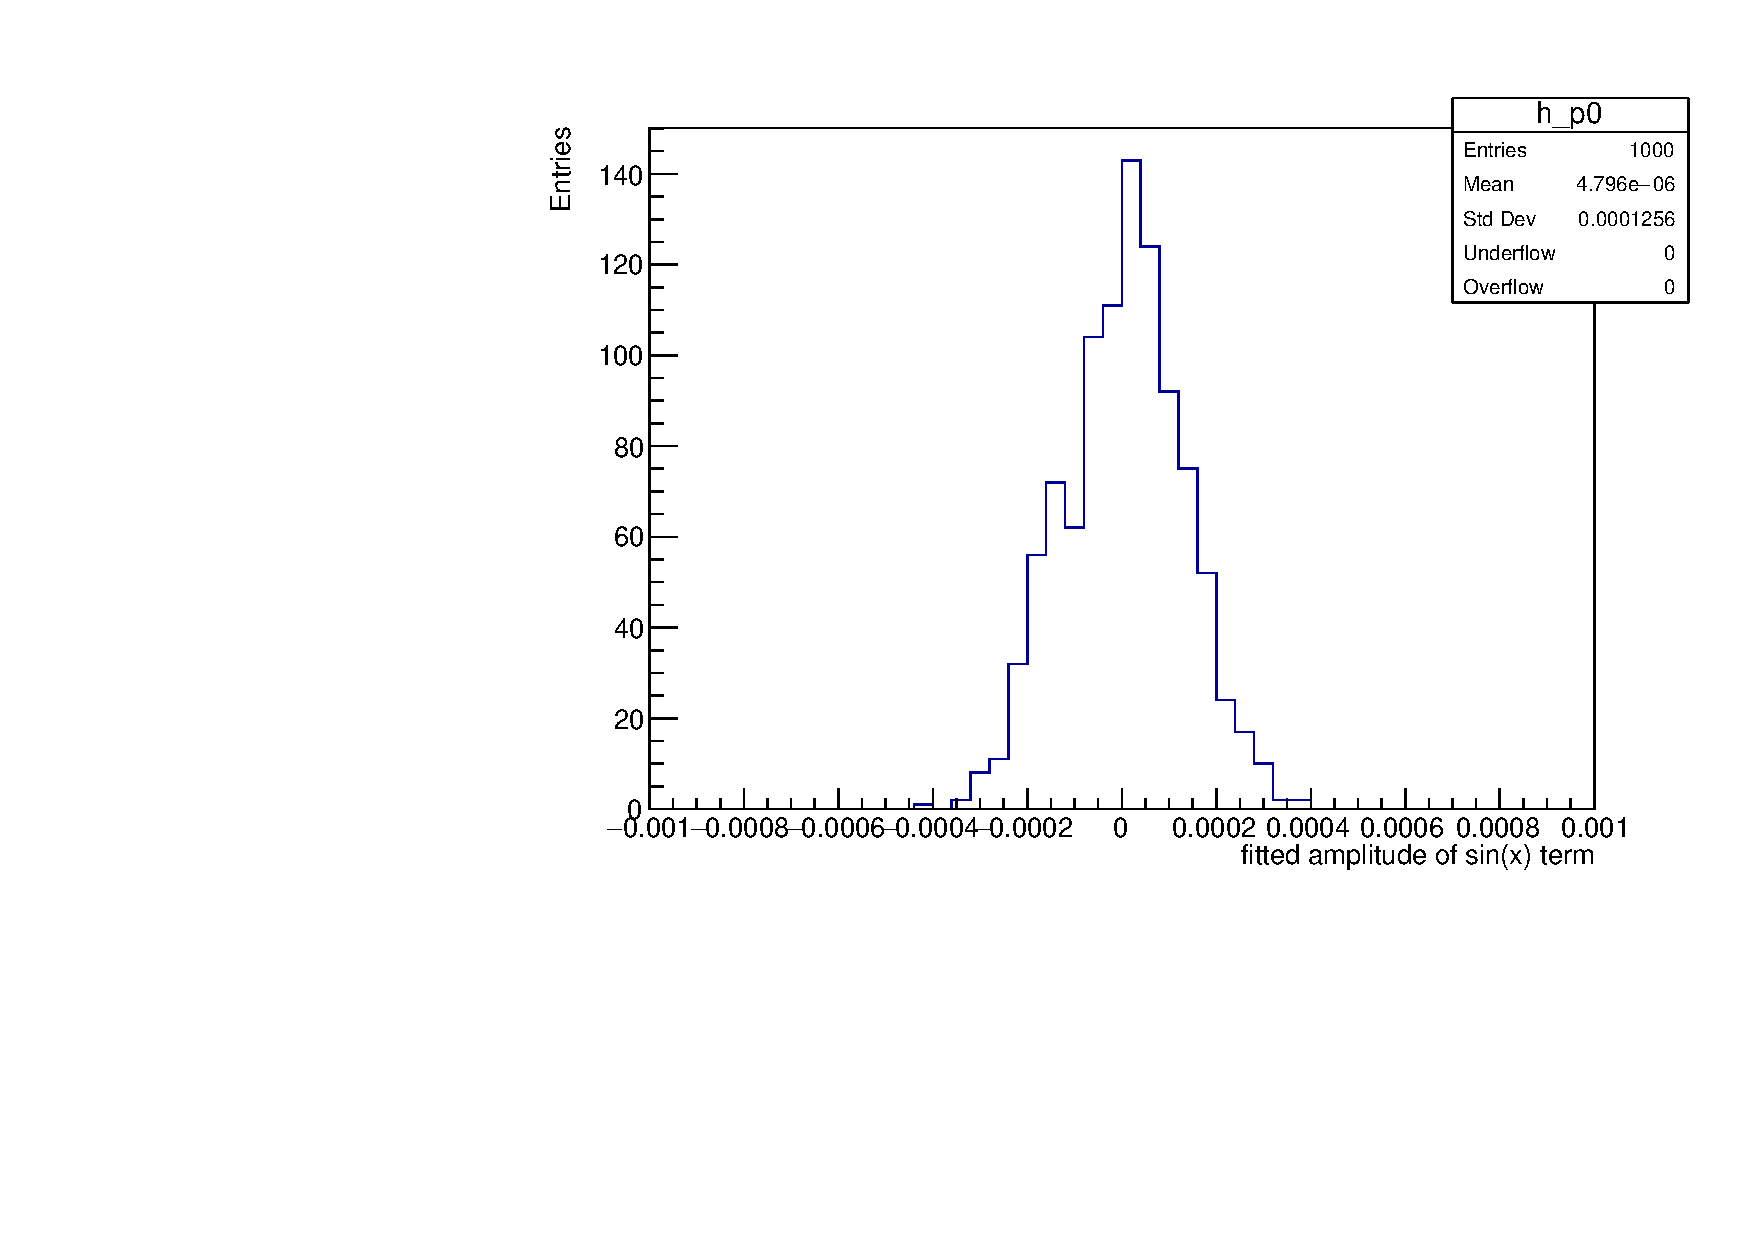
\includegraphics[width=0.4\textwidth]{figs/toy/res_1000_toy_nosignal_p0.pdf}
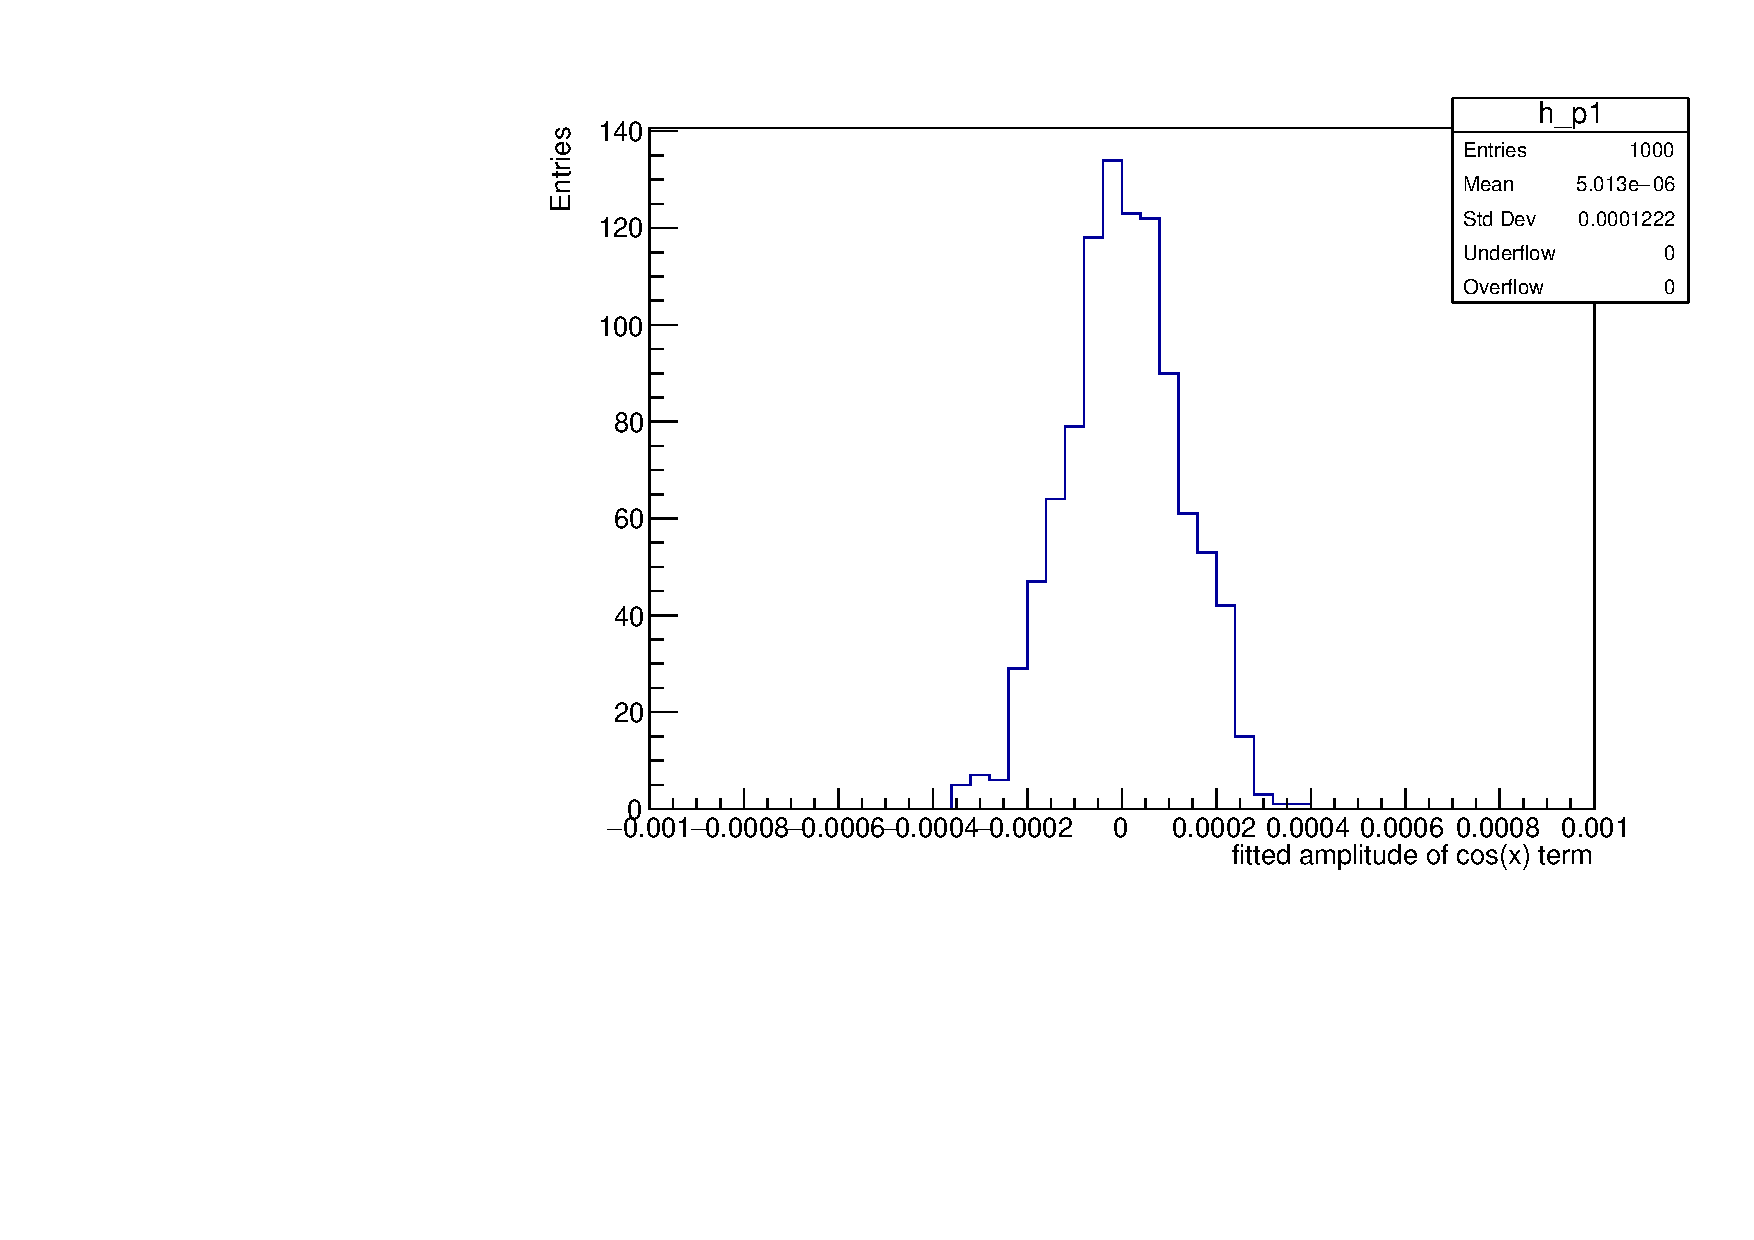
\includegraphics[width=0.4\textwidth]{figs/toy/res_1000_toy_nosignal_p1.pdf}
\caption{\label{fig:toy_1000exp_s0pb} Result of 1000 toy experiement with NULL signal. Fit function is 1 + p0 sin(x)+p1 cos(x). (left) amplitude of sin(x) term, (right) amplitude of cos(x). }
\end{figure}

%\clearpage
%% \subsection{Null hypothesis test}
\label{sec:null_test}

%% Null test is that we perform a fit to data (toy datasets) using SM expectation. 
%% The SM expectation is a flat distribution in which free parameter is an offset (e.g $y = c $).

In this test, 1000 toy datasets generated with SM expection and corresponds 
to Run 2 datase are used. In another words, no signal is injected to these datasets.

Figure~\ref{fig:null_test} show distributions of fit parameters, errors,
$\chi^{2}/ndf$ (ndf is number of degree of freedom) and  $p_{0}$ value of
$\chi^{2}$, from fitting a flat distribution (bkg expection) to the 1000
toy datasets. Since the obserable is a Double Ratio, the fitted off-set (fit parameter)
is allways one in each fit. The normalzed $\chi^{2}$ ($\chi^{2}/ndf$, bottom right plot)
distribution is centered around one which means the toy datasets agree
with a flat distribution (this is what we expected). If we take  $p_0$ > 0.01 as a threshold to determine
if the dataset agree with the SM expectation (flat distribution), then more then 99\% of the toy dataset
passed this cut ($p_0$ > 0.01 ). Since more then 99\% of the samples agree with SM expectation we can conclude
that random fluctuation can not introduce strange shapes that significantly different then a flat distribution.

\begin{figure}[!htb]
  \centering
  \subfloat{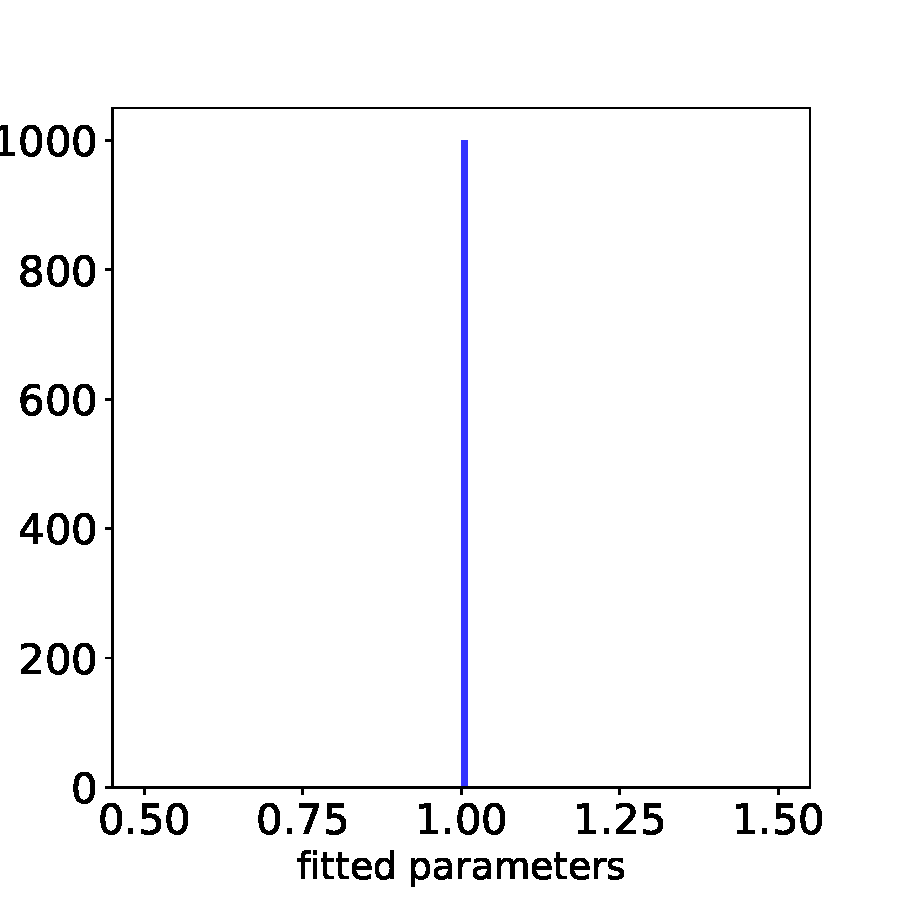
\includegraphics[width=0.40\textwidth]{figs/null_test/Null_test_pars}}
  \subfloat{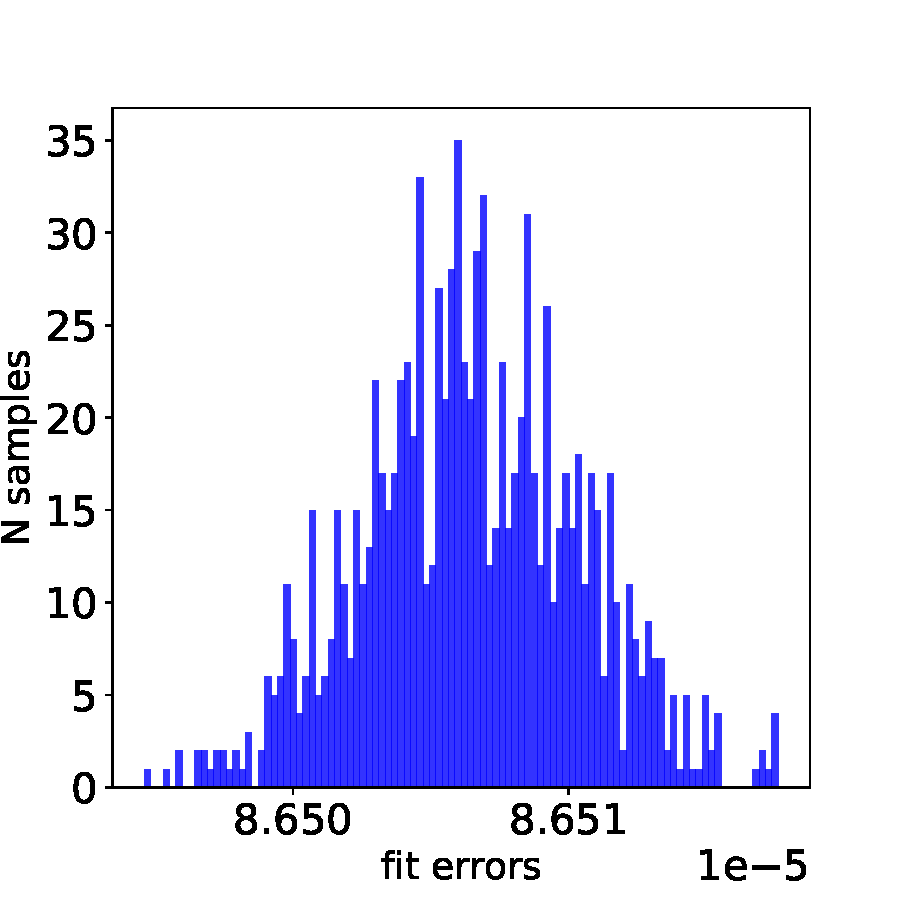
\includegraphics[width=0.40\textwidth]{figs/null_test/Null_test_err}}\\
  \subfloat{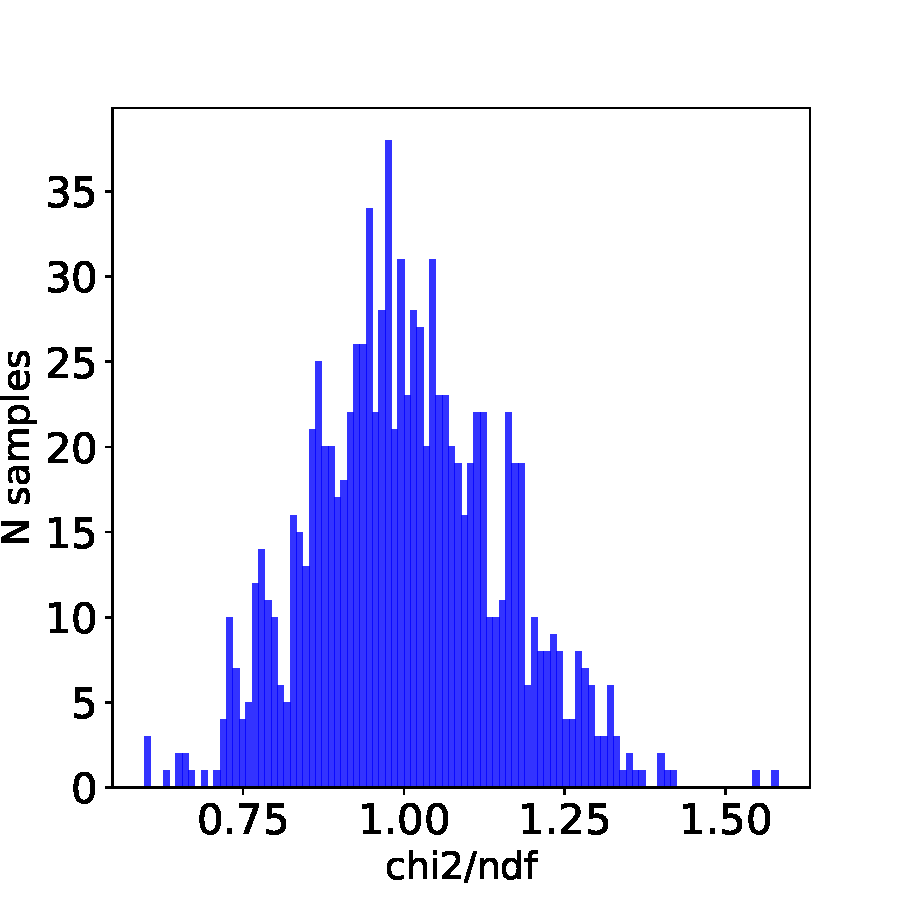
\includegraphics[width=0.40\textwidth]{figs/null_test/Null_test_chi2_ndf}}
  \subfloat{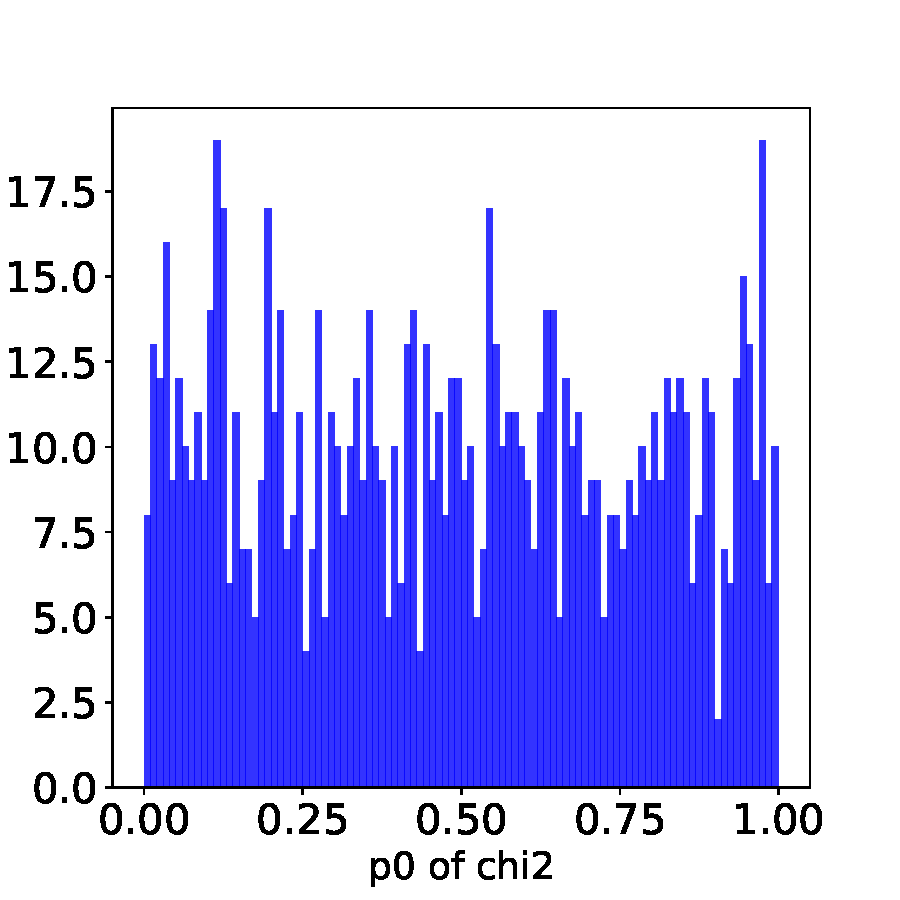
\includegraphics[width=0.40\textwidth]{figs/null_test/Null_test_chi2_p0}}
  \caption{Results of Null Tests on 1000 signal-free toy datasets. Top left plot is estimated parameters, top right is fit errors, bottom left is $\chi^{2}/ndf$ (ndf is number of degree of freedom), bottom right is $p_{0}$ of $\chi^{2}$.}
  \label{fig:null_test}
\end{figure}



%\clearpage
\subsection{Spurious signal test}
\label{sec:spurious_test}

Spurious signals may occur from statistical fluctuations. Therefore, in this section, we test toy datasets to check if there are signal like structures. The toy datasets are signal-free datasets (no signals injected), and generated total of 1000 samples. Each sample (toy dataset) is fitted 12 times, each time with different signal shapes (we have total of 12 signals). Each fit will estimate a coefficient. 

Figure~\ref{fig:spurious_test} shows distributions of 4 example coefficients ($d_u^{XZ}\equiv d_{0}$, $d_u^{YZ} \equiv d_{1}$, $d_u^{XX-YY} \equiv d_{2}$ and $d_u^{XY} \equiv d_{3}$) estimated from 1000 toy datasets. From each plot we can see that mean of each distribution is very close to zero. The Figure~\ref{fig:spurious_test_summary} shows mean and standard deviation of the distributions shown in Figure~\ref{fig:spurious_test}, expanded to all 12 coefficients.



\begin{figure}[!htb]
	\centering
	\subfloat{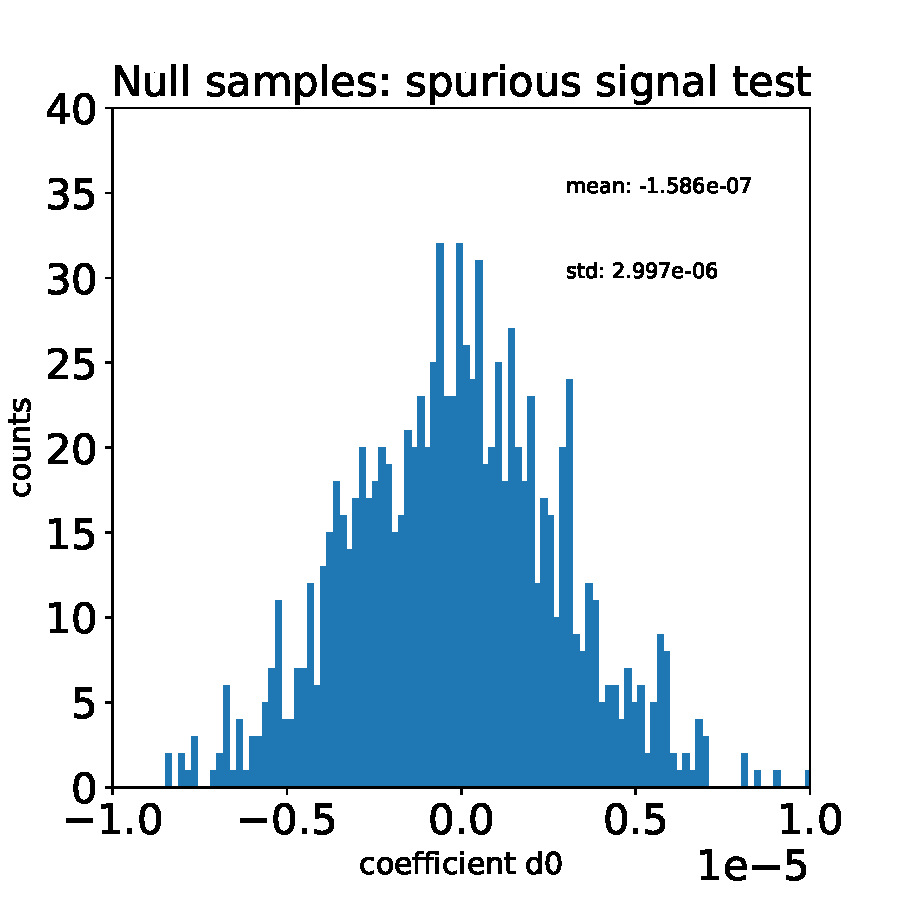
\includegraphics[width=0.48\textwidth]{figs/spurious_test/Null_spurious_test_d0}}
	\subfloat{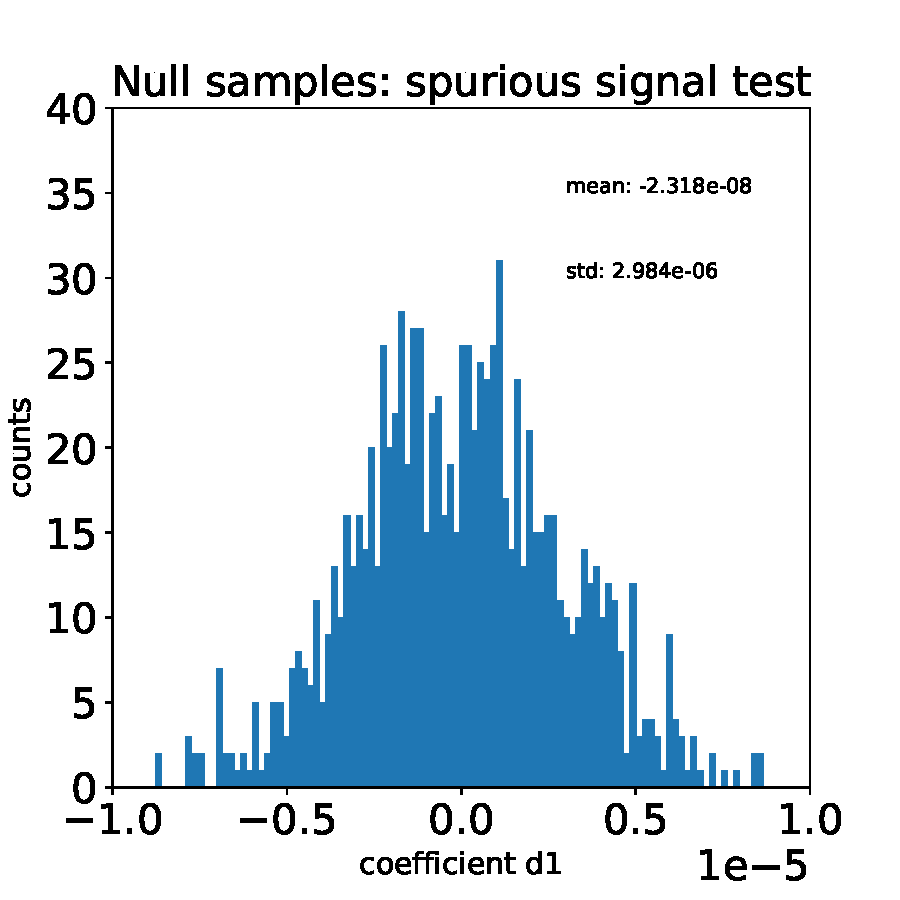
\includegraphics[width=0.48\textwidth]{figs/spurious_test/Null_spurious_test_d1}}\\
	\subfloat{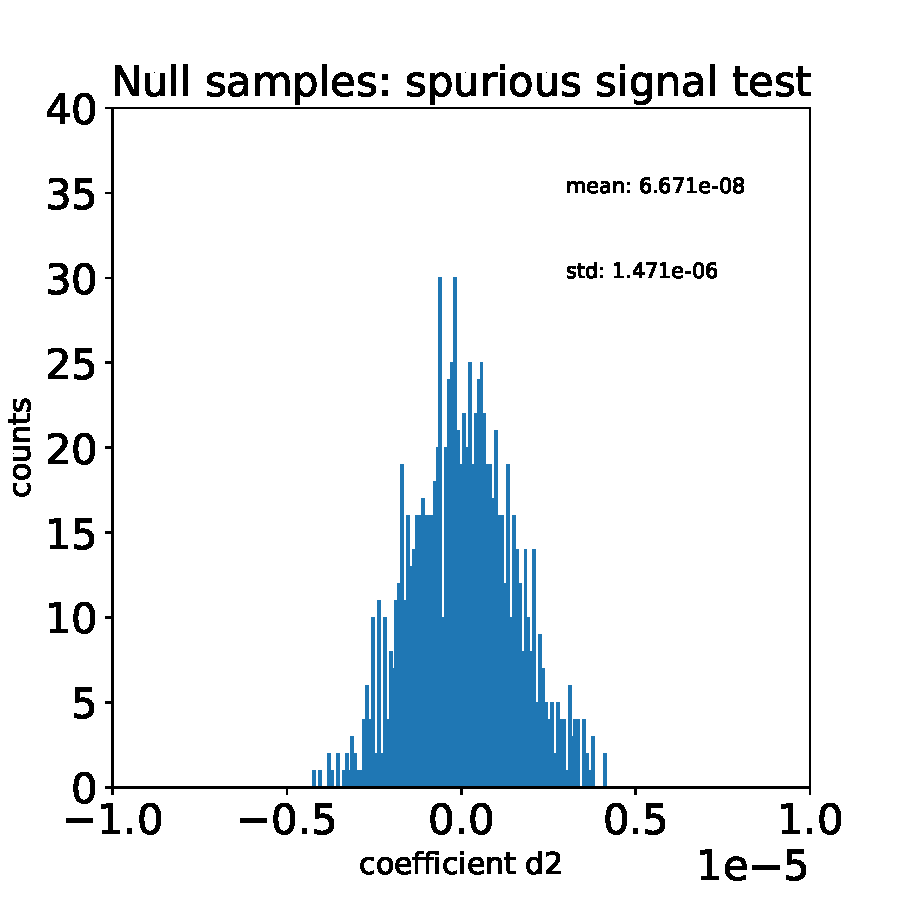
\includegraphics[width=0.48\textwidth]{figs/spurious_test/Null_spurious_test_d2}}
	\subfloat{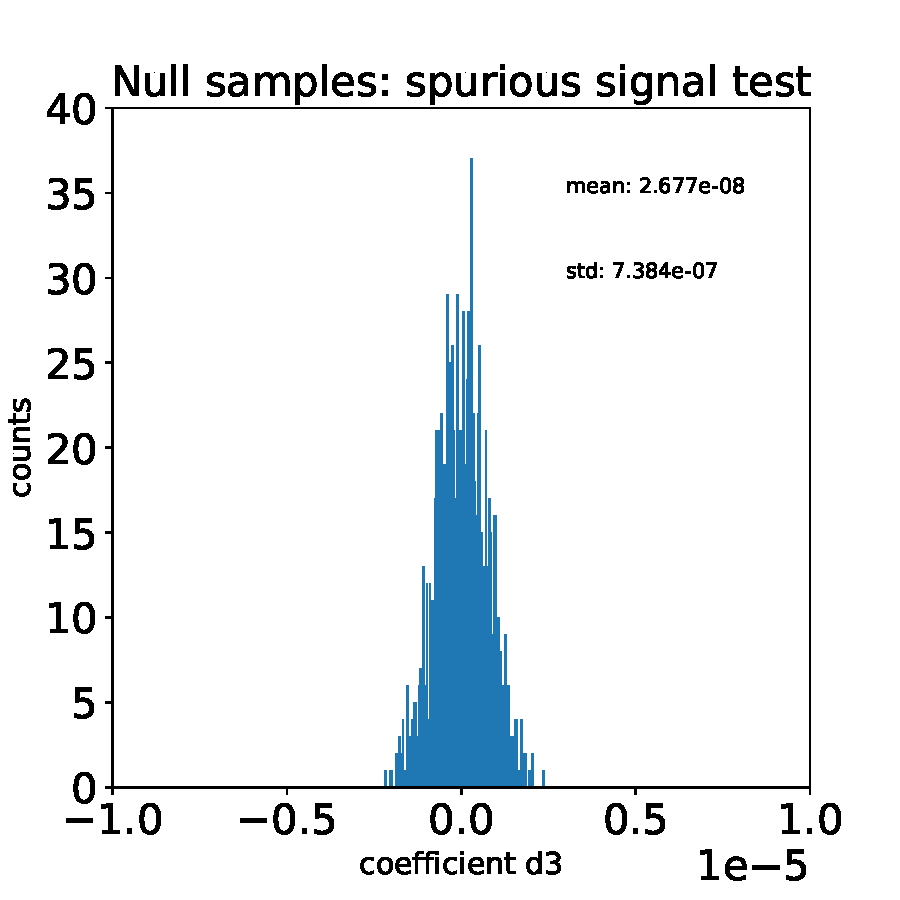
\includegraphics[width=0.48\textwidth]{figs/spurious_test/Null_spurious_test_d3}}
    \caption{Results of spurious signal tests on 1000 signal-free toy datasets. Top left is a distribution of estimated $d_{0}$ parameters, top right is $d_{1}$ parameters, bottom left is $d_{2}$ parameters and bottom right is $d_{3}$ parameters.}
	\label{fig:spurious_test}
\end{figure}


\begin{figure}[!htb]
	\centering
	\subfloat{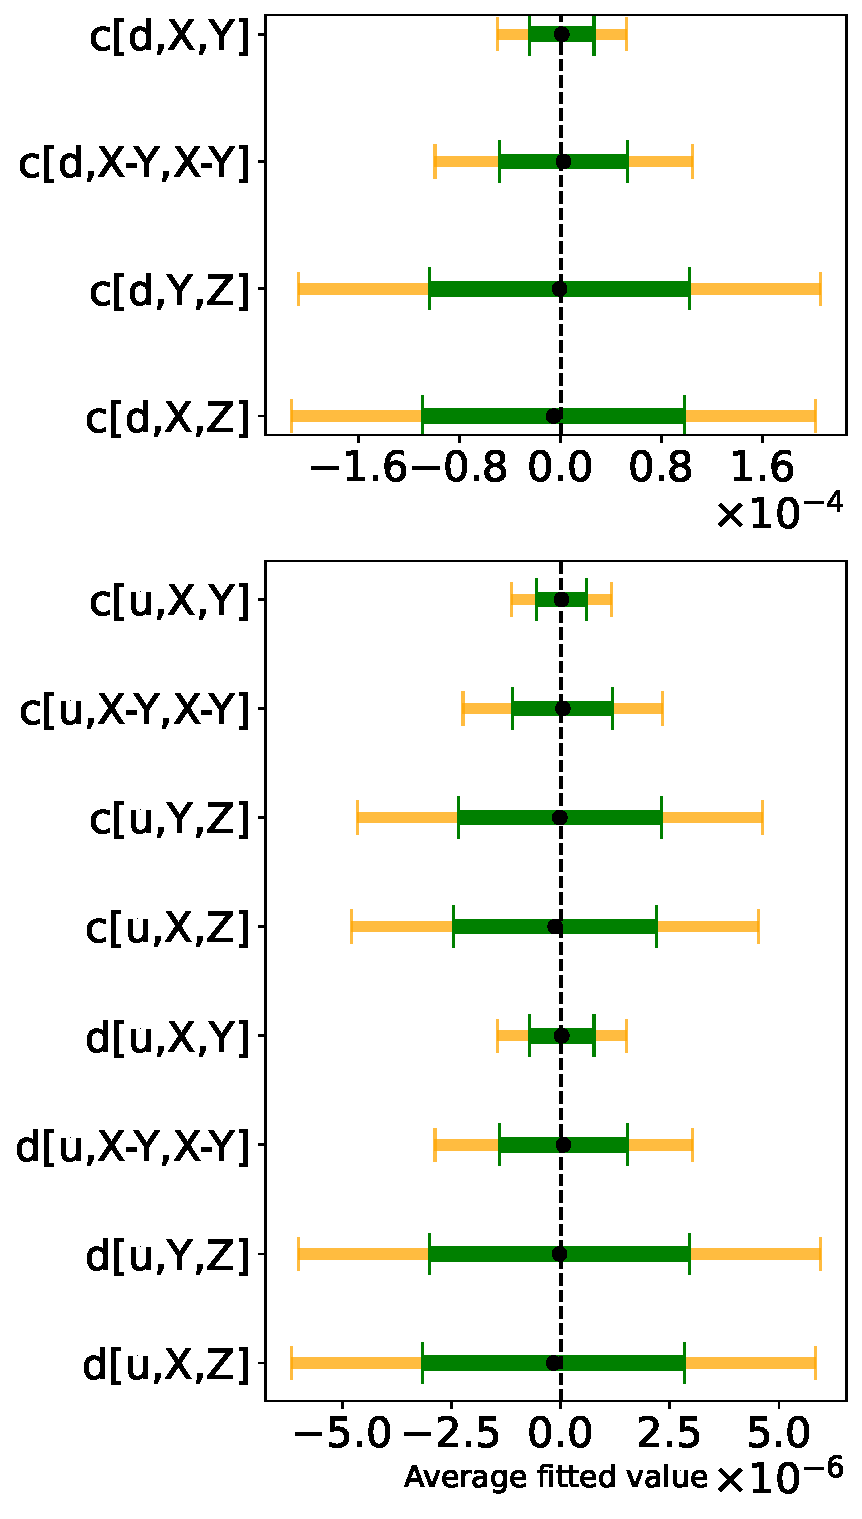
\includegraphics[width=0.48\textwidth]{figs/spurious_test/Null_SigFit_summary_1000samples}}

     \caption{Summary of spurious signal tests on 1000 signal-free toy datasets. Black dot is a numpy mean of corresponding distributions
       in the Figure~\ref{fig:spurious_test}, the green and orange bands are one and two standard diviations calculated with the numpy function. }
	\label{fig:spurious_test_summary}
\end{figure}



\subsubsection{Simple LIV effect}

 This is test with LIV signal amplitude of 1 pb with sin curve. 
Same as NULL case, 1000 toy experiments are generated as same method described in Section~\ref{sec:basic_TOYmodel}, and fitted with simple function. Results are shown in Fig.~\ref{fig:toy_1000exp_s1pb}
The mean of the fitted amplitude of sin (cos) term is 0.0013 (0.000), which is consistent with generated configuration. 

\begin{figure}
\centering
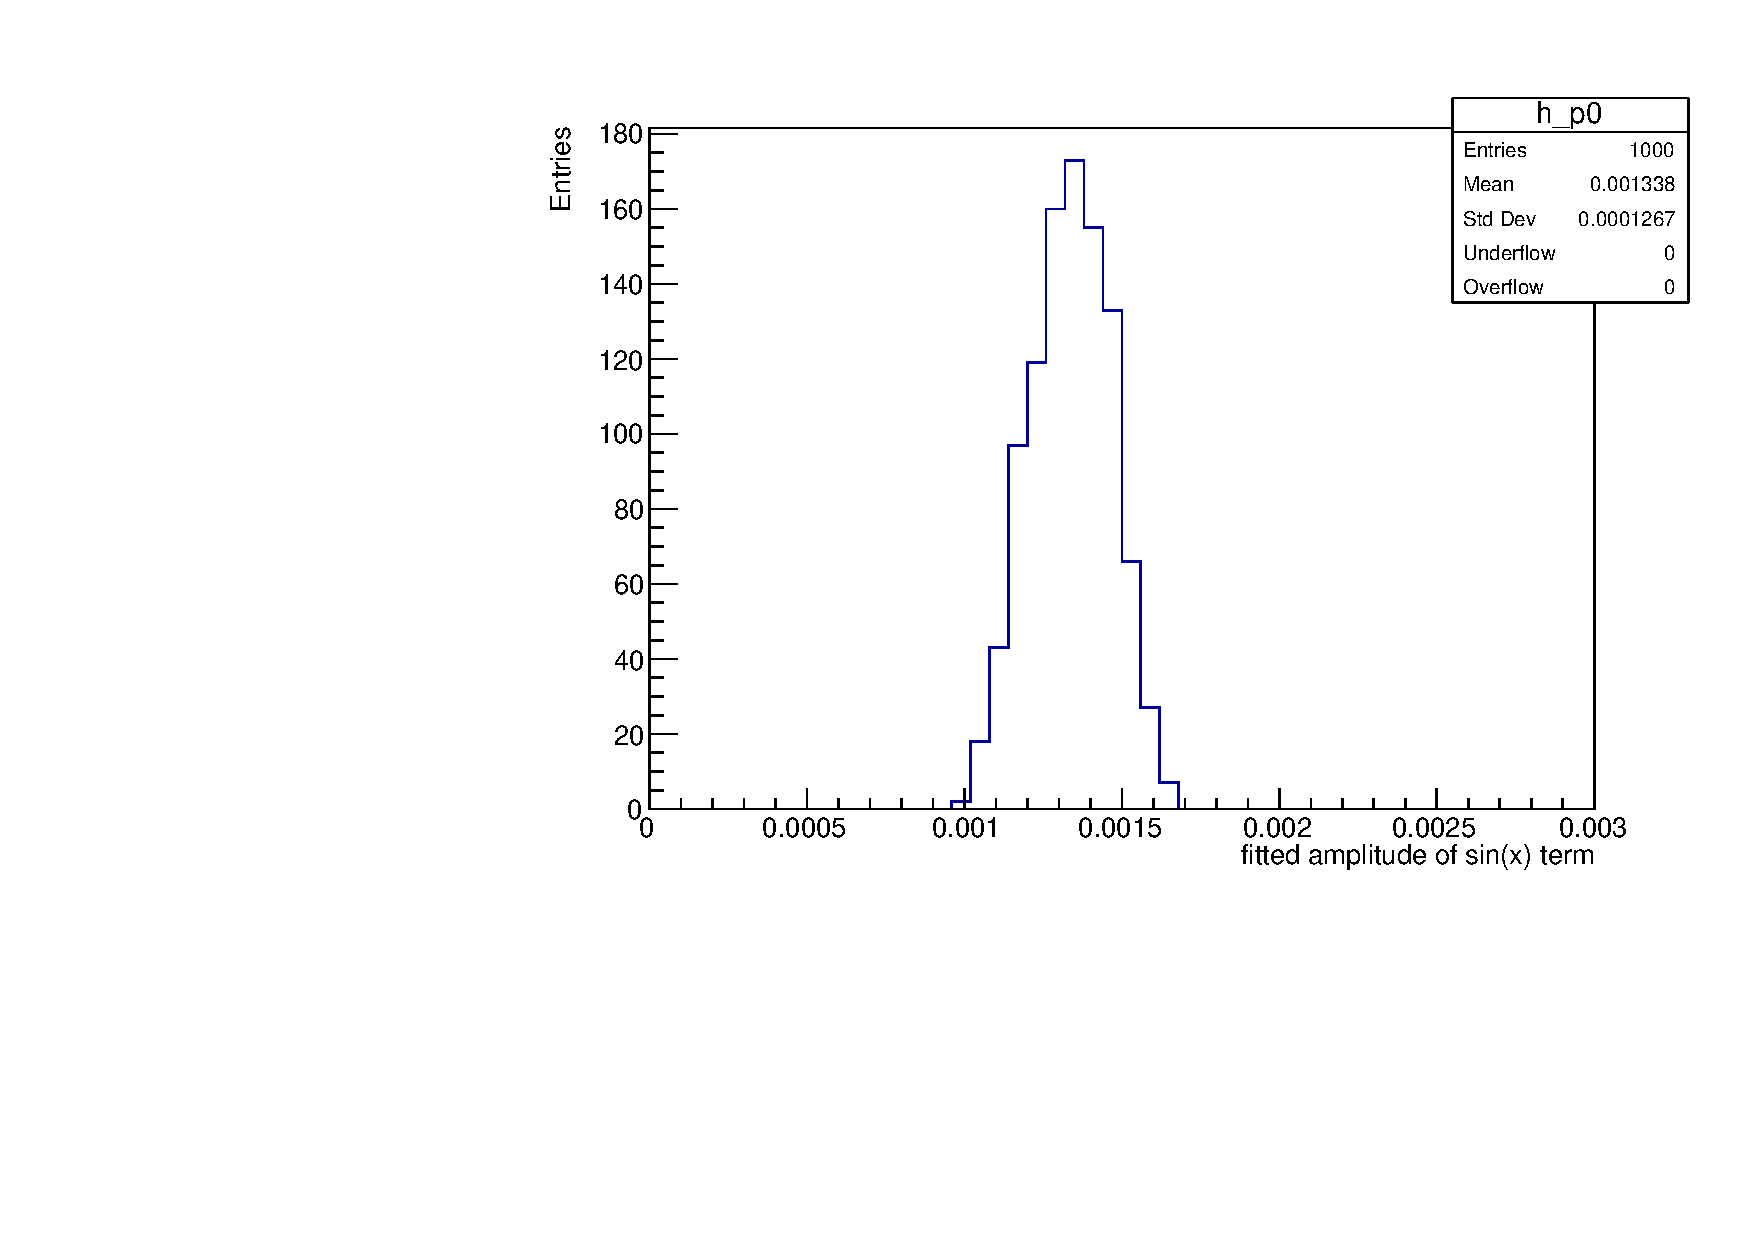
\includegraphics[width=0.4\textwidth]{figs/toy/res_1000_toy_p0.pdf}
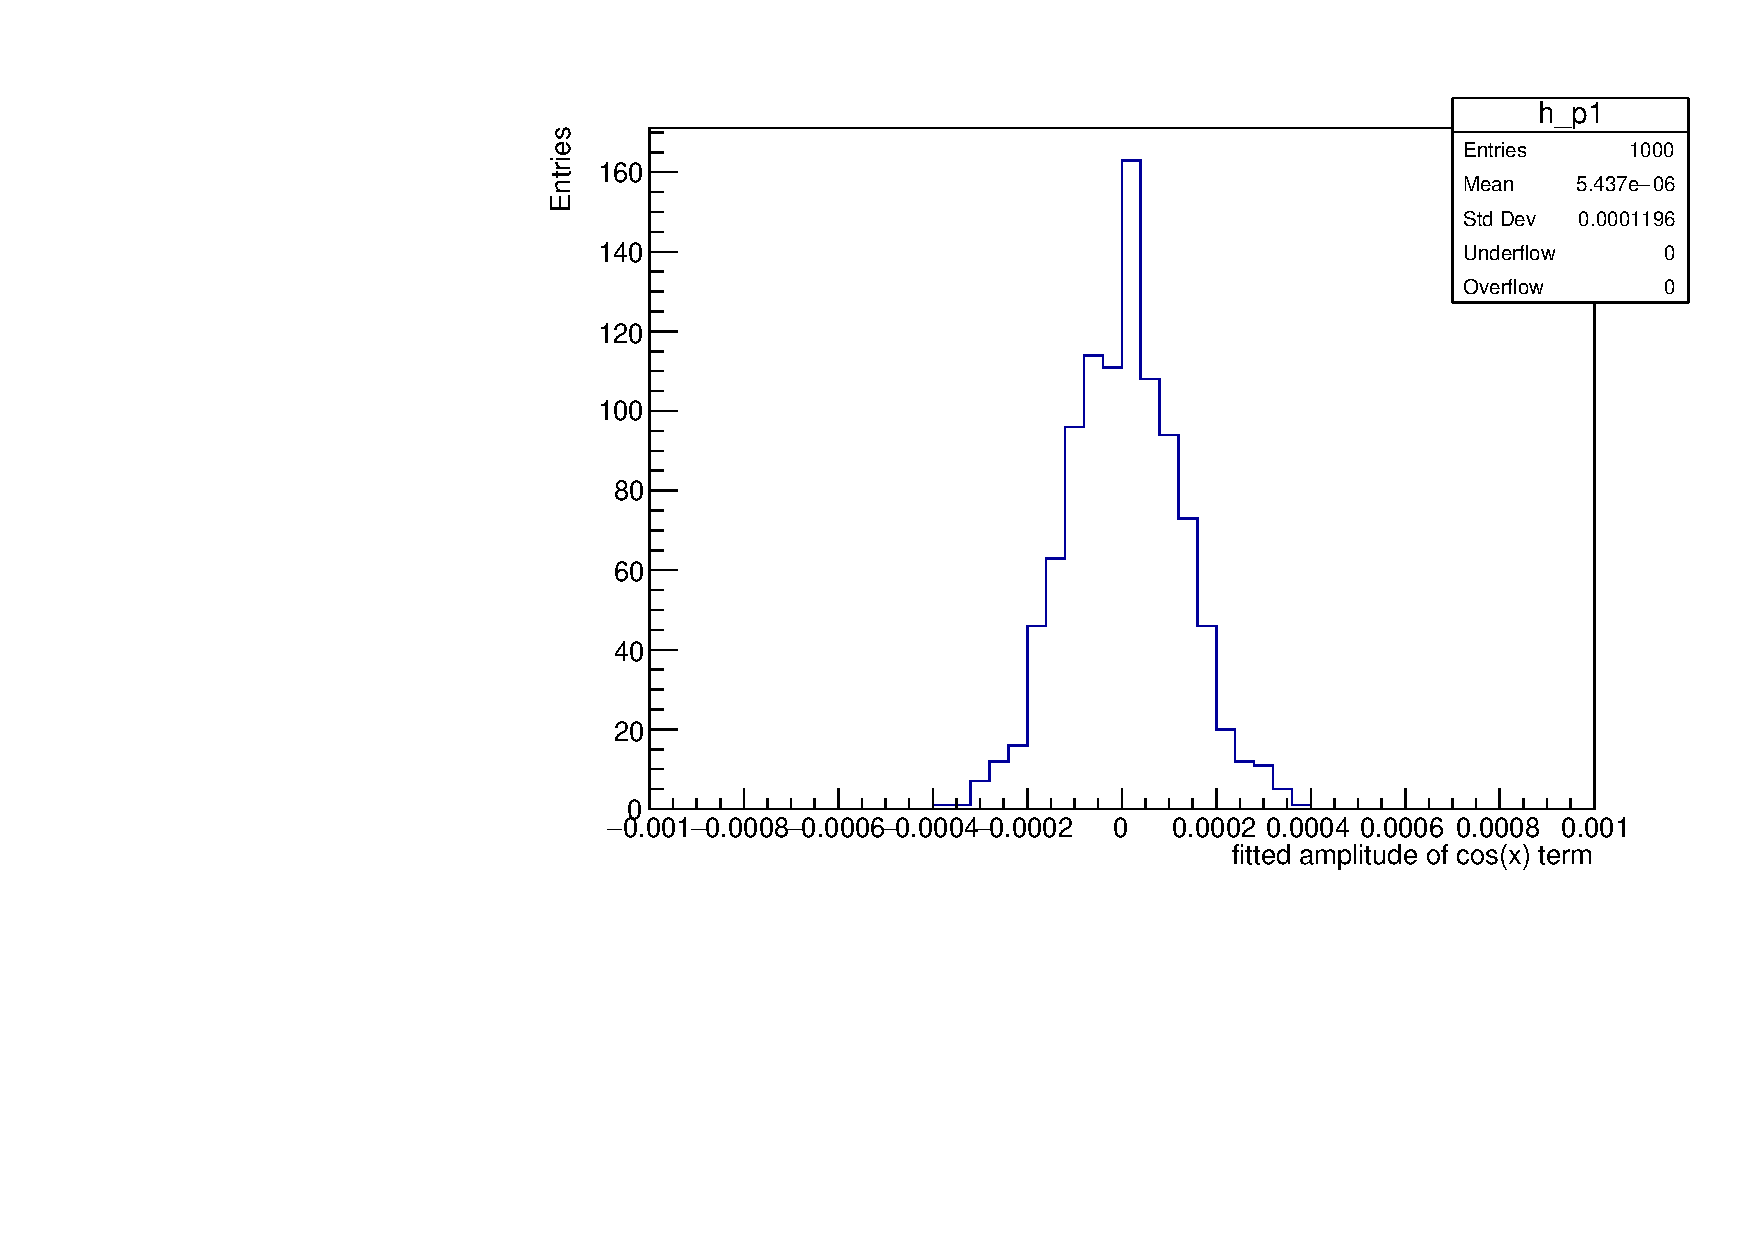
\includegraphics[width=0.4\textwidth]{figs/toy/res_1000_toy_p1.pdf}
\caption{\label{fig:toy_1000exp_s1pb} Result of 1000 toy experiement with LIV signal amplitude of 1 pb. Fit function is 1 + p0 sin(x)+p1 cos(x). 
(left) amplitude of sin(x) term, (right) amplitude of cos(x). }
\end{figure}

Figure~\ref{fig:toy_1000exp_s03pb} shows same set of result close to 3 sigma level sensitivity (only taken into account statistics uncertainty). 
The injected signal amplitude is 300 fb.

\begin{figure}
\centering
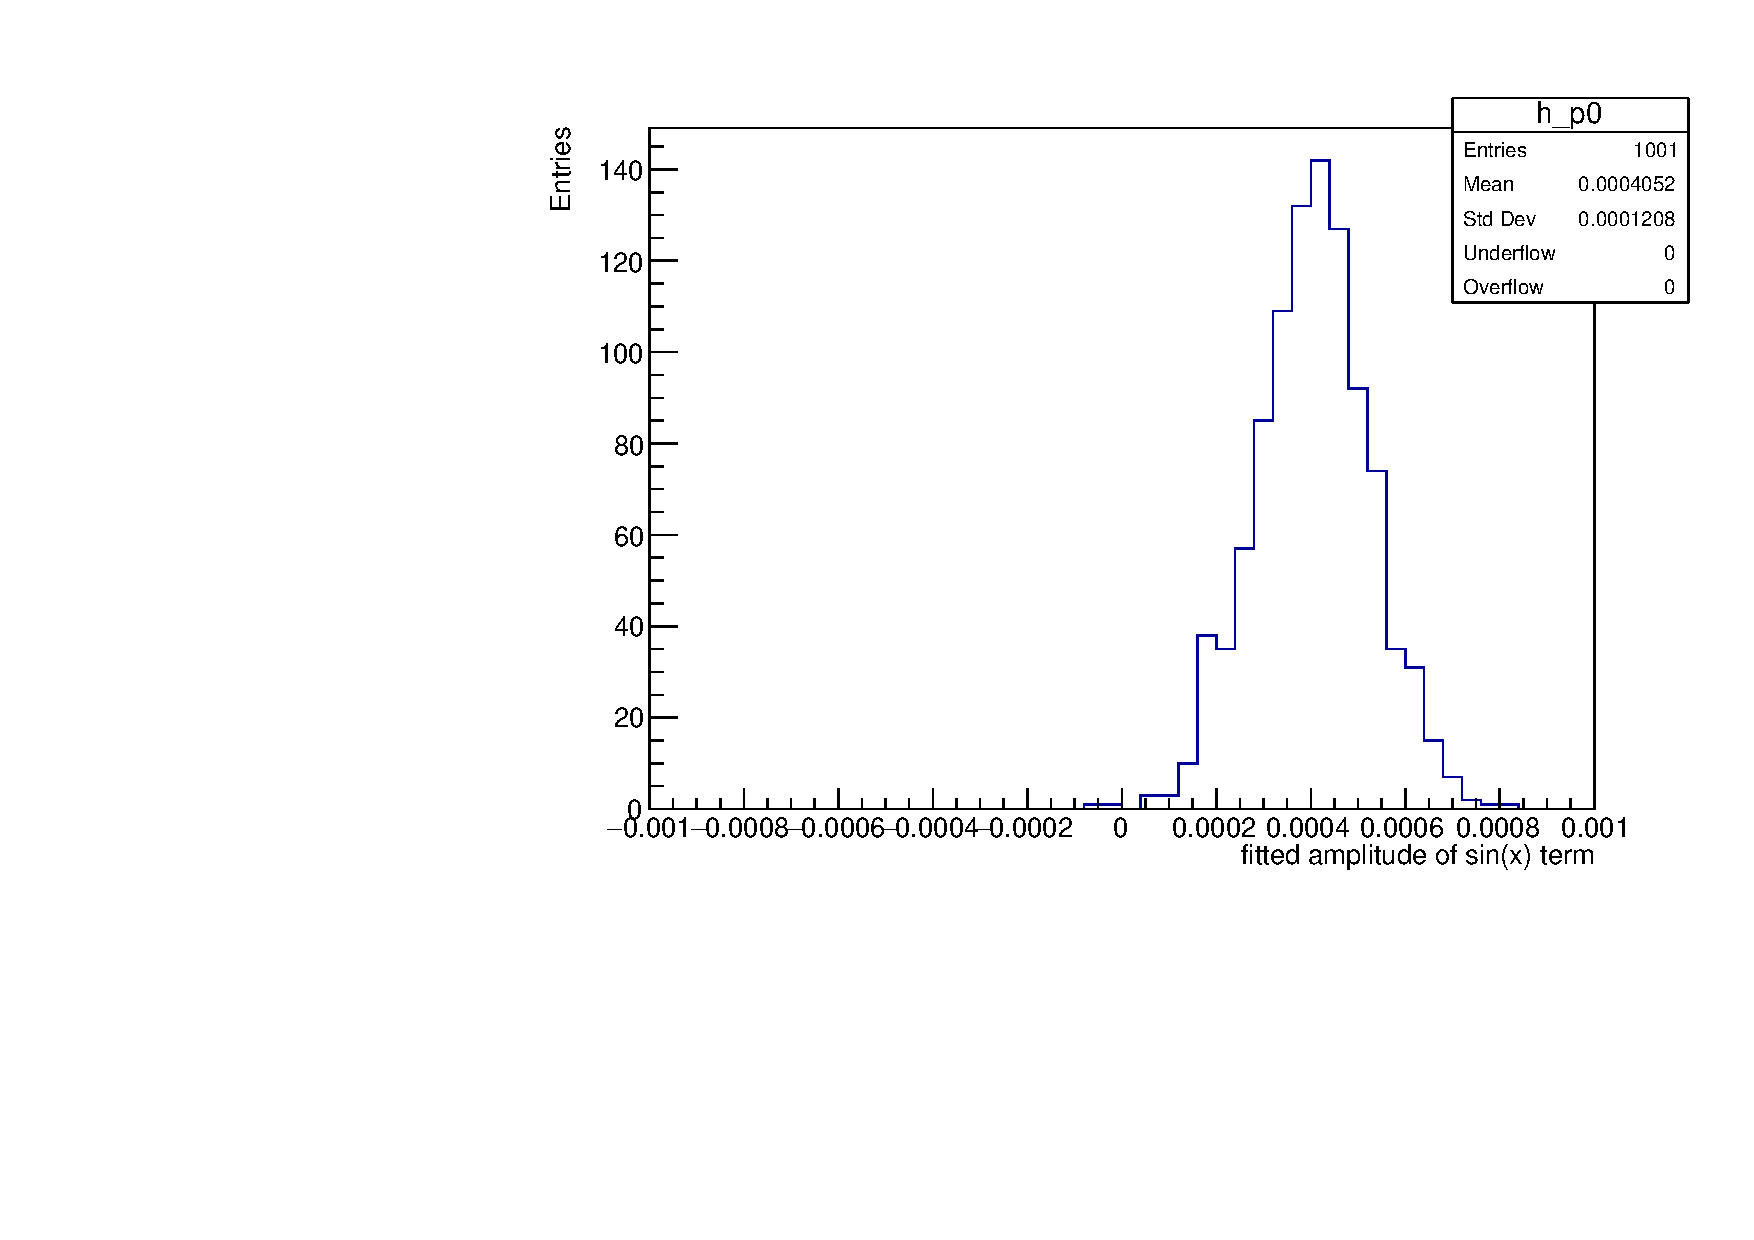
\includegraphics[width=0.4\textwidth]{figs/toy/res_1000_toy_sig0p3_p0.pdf}
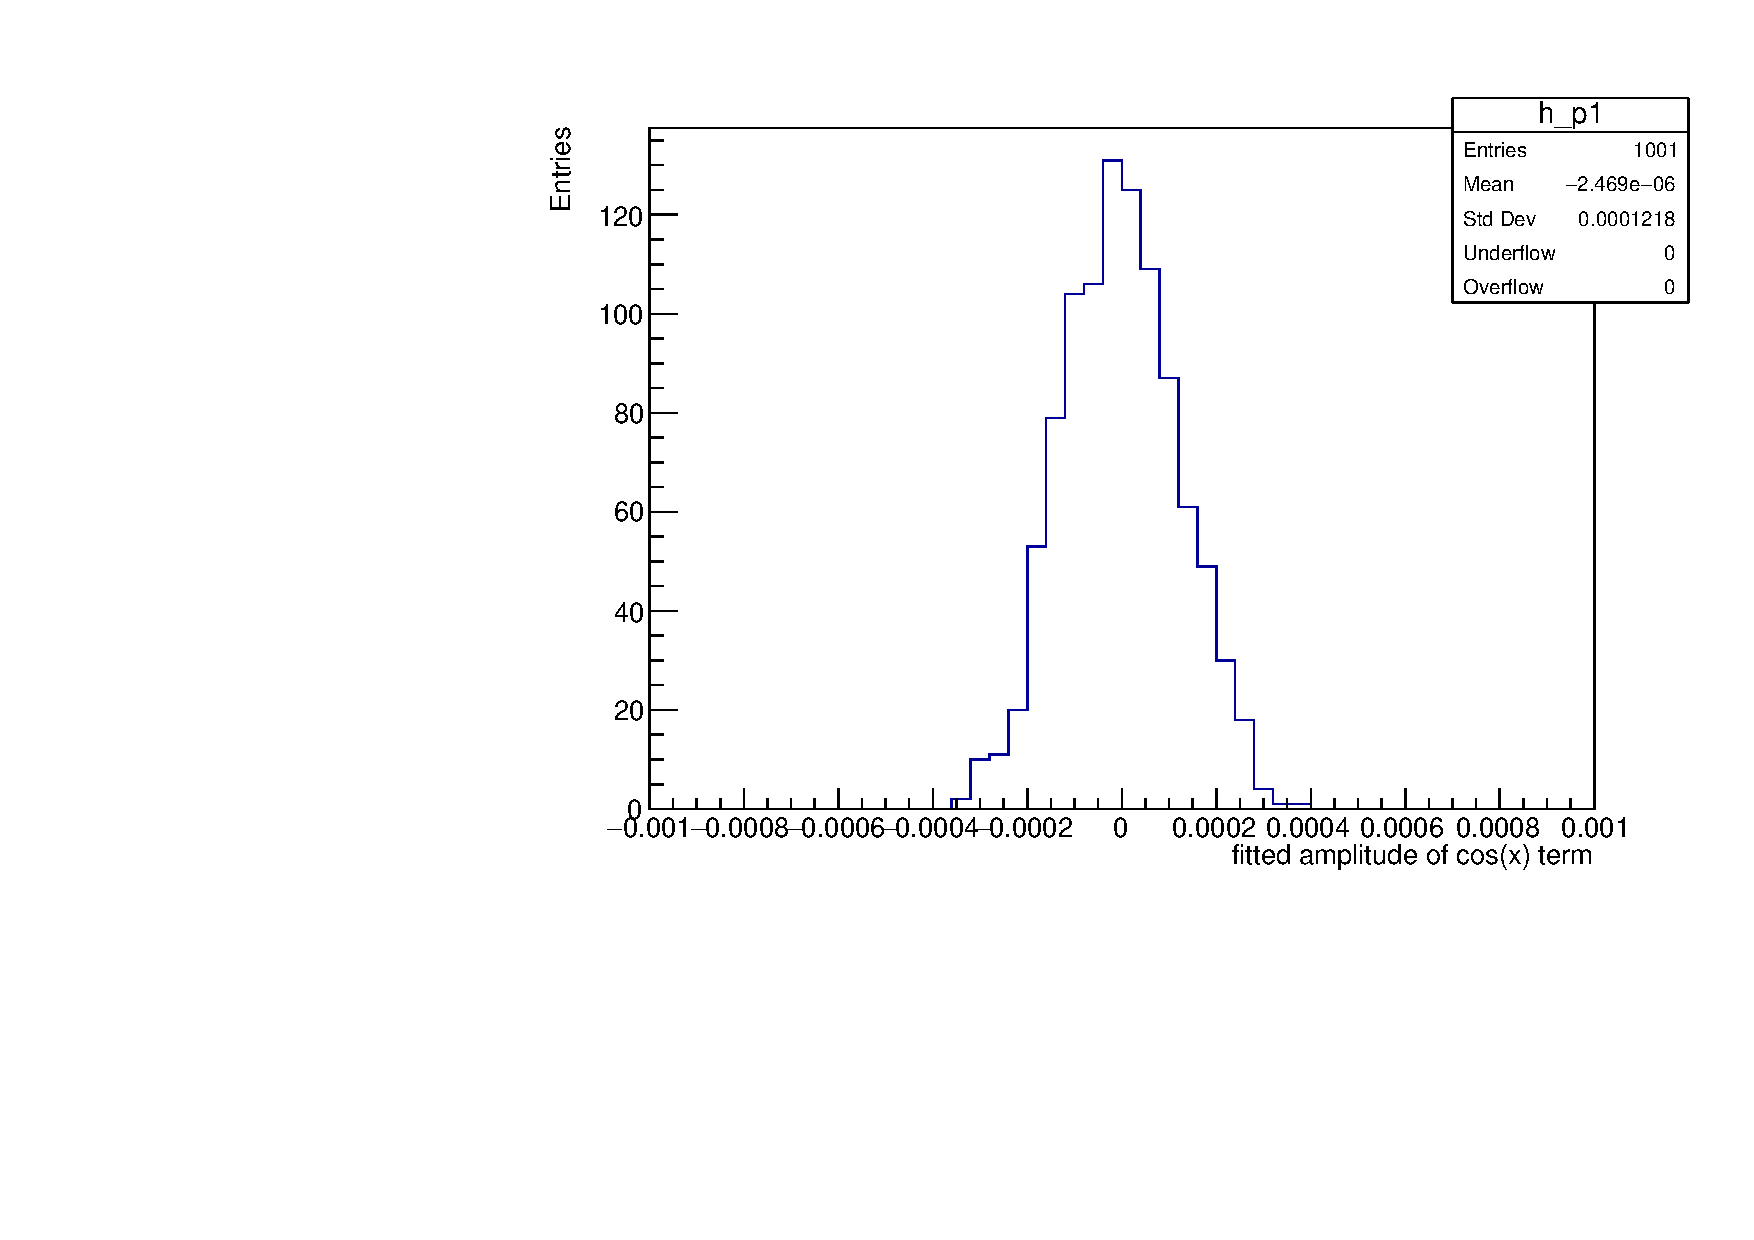
\includegraphics[width=0.4\textwidth]{figs/toy/res_1000_toy_sig0p3_p1.pdf}
\caption{\label{fig:toy_1000exp_s03pb} Result of 1000 toy experiement with LIV signal amplitude of 0.3 pb. Fit function is 1 + p0 sin(x)+p1 cos(x). 
(left) amplitude of sin(x) term, (right) amplitude of cos(x). }
\end{figure}


\subsubsection{Number of bin in sidereal phase}
\label{sec:number_of_bins}
 Number of binning in sidereal phase is scanned with simple Toy. Result is shown in Fig.~\ref{fig:toy_sig_nbins_liv_1pb}, 
which is performed with LIV signal amplitude of 1 pb. As expecdted, low number of bins shows low significance, 
this is just simply cancel negative part and positive part of signal due to coarse binning.
An interesting observation is there are small bias around number of bins from 10 to 15. It has higher than reaching plateau, after number of bins greater than 25. 
This indicates it's better to use enough large number of bins. For finer direction, the Run-2 data provides a large number of Z events, therefore we could use very fine binning. 
Finest limit case would be 1440, which is based on duration of LB (60 seconds) over 24 hours. 
To avoid too fine bin, we choose number of bins of 100 as the default configuration. Here 1 bin corresponds to about 15 min duration for the sidereal phase.

\begin{figure}
\centering
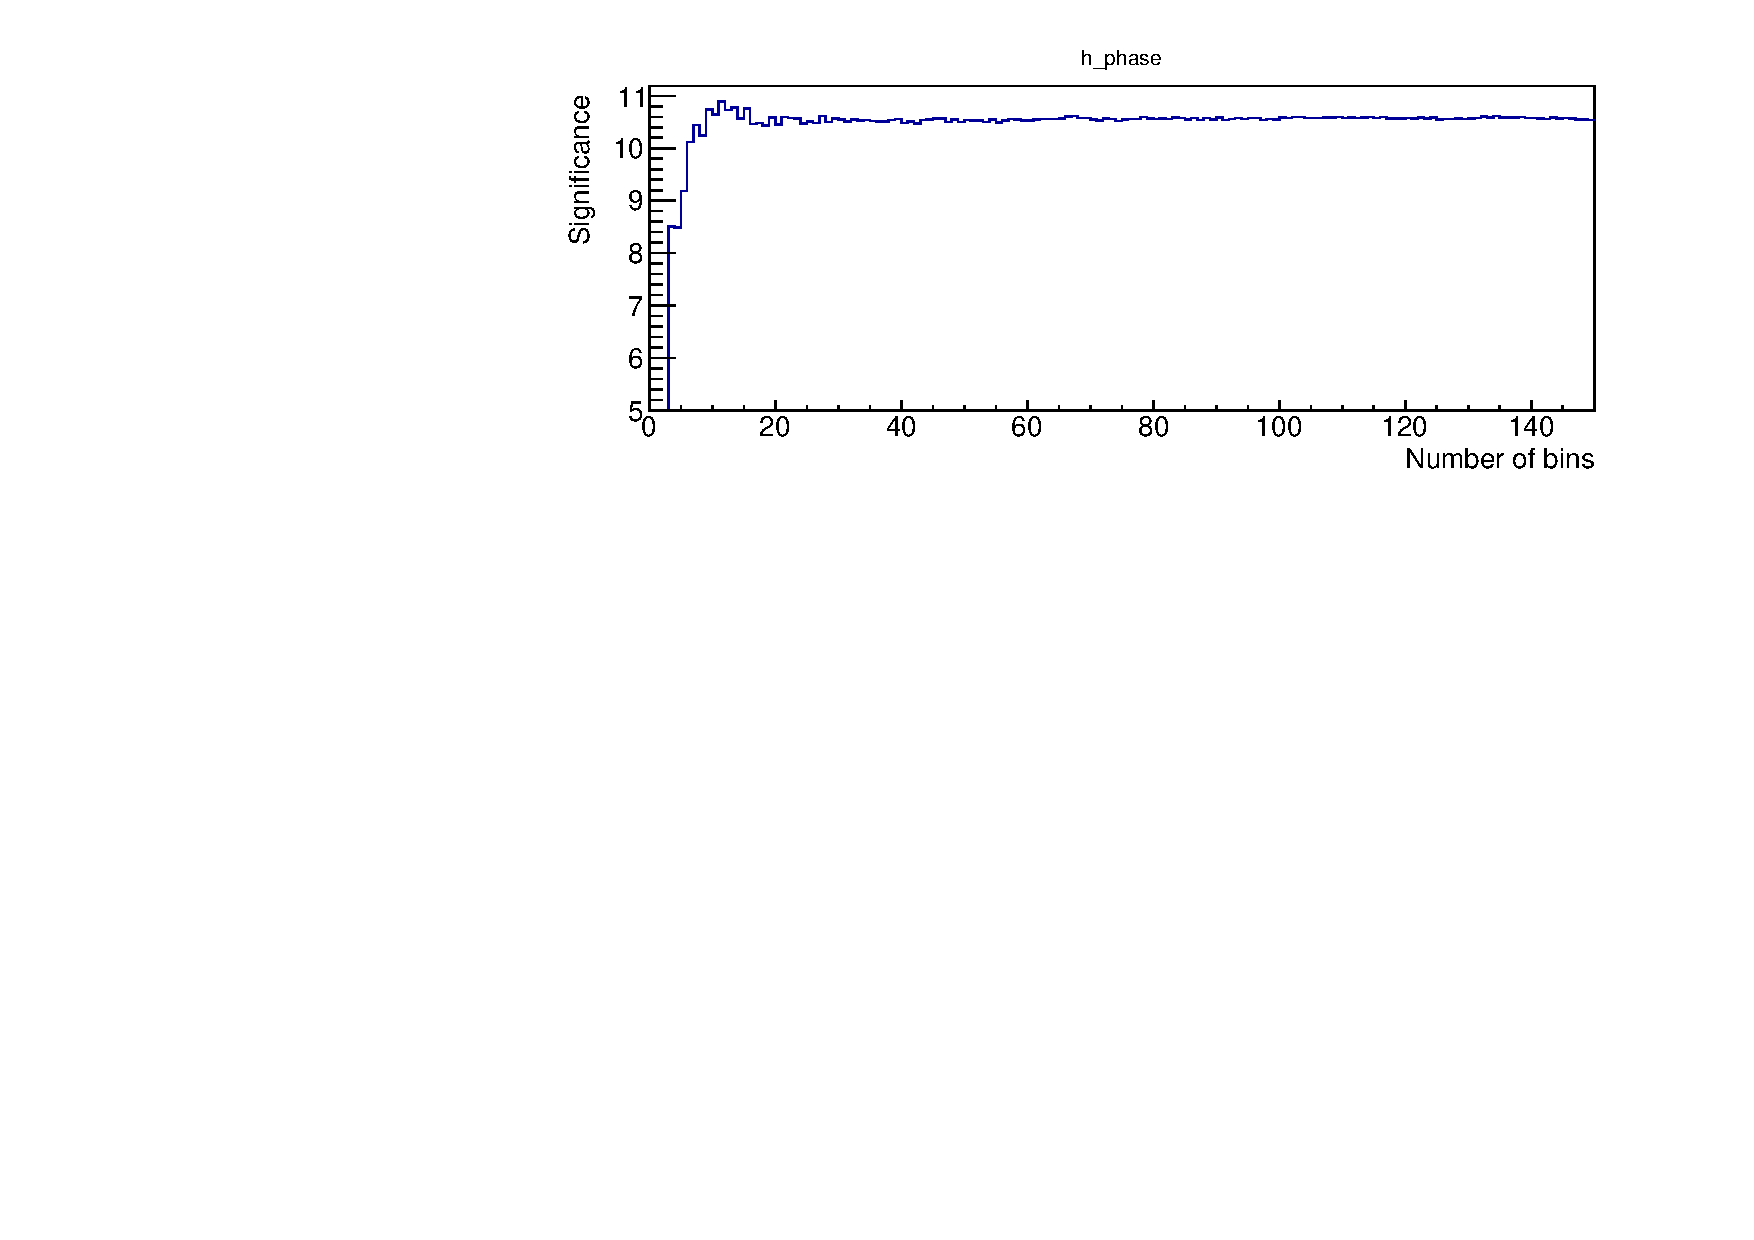
\includegraphics[width=0.8\textwidth]{figs/toy/sig_nbins_liv_1pb.pdf}
\caption{\label{fig:toy_sig_nbins_liv_1pb} Significance (quadrature sum of diviataion from 1 on the double ratio in sidereal 100 bins) as function of number of bins with no random case. Injected LIV amplitude is 1 pb. }
\end{figure}


\subsubsection{Changing probing sidereal period for expected signal}

 This study was made to check if we could check day-night effect. The difference of duration between solar day and the sidereal day is about 4 minutes, 
which corresponds to only $\sim 0.3$\%.  Looking the day-night effect may be effectively reveal the potential LIV effect. Fig.~\ref{fig:toy_sig_periodscale_zoom} 
confirms this hypothesis, we would see LIV signal with probing period with the solar day. In this test, inject signal amplitude is 1 pb sin curve with sidereal phase. 
And the significance is computed by changing the probing period scale factor, $\alpha_{preriod}$. Here the $\alpha_{preriod}$ is 
the scale factor on the period to compute phase. To have the period of solar day, $\alpha_{preriod}$ is 1.00274.  
In the figure, $\alpha_{preriod}$ is scanned from 0.975 to 1.025. Observed periodic peak structure.  Wider range of scan is shown in Fig.~\ref{fig:toy_sig_periodscale}. 

Base on this study, we understood we should not look the double ratio with the period of solar day in order to make blind data analysis.
We are planning to make step by step unblinding. Once all studies are performed, start to make fit on the double ratio with the probing phase of 1 hour and 7 hours.
%% More description on blinding strategy are discussed in Section.~\ref{sec:step_by_step_unblind_test}.
 
\begin{figure}
\centering
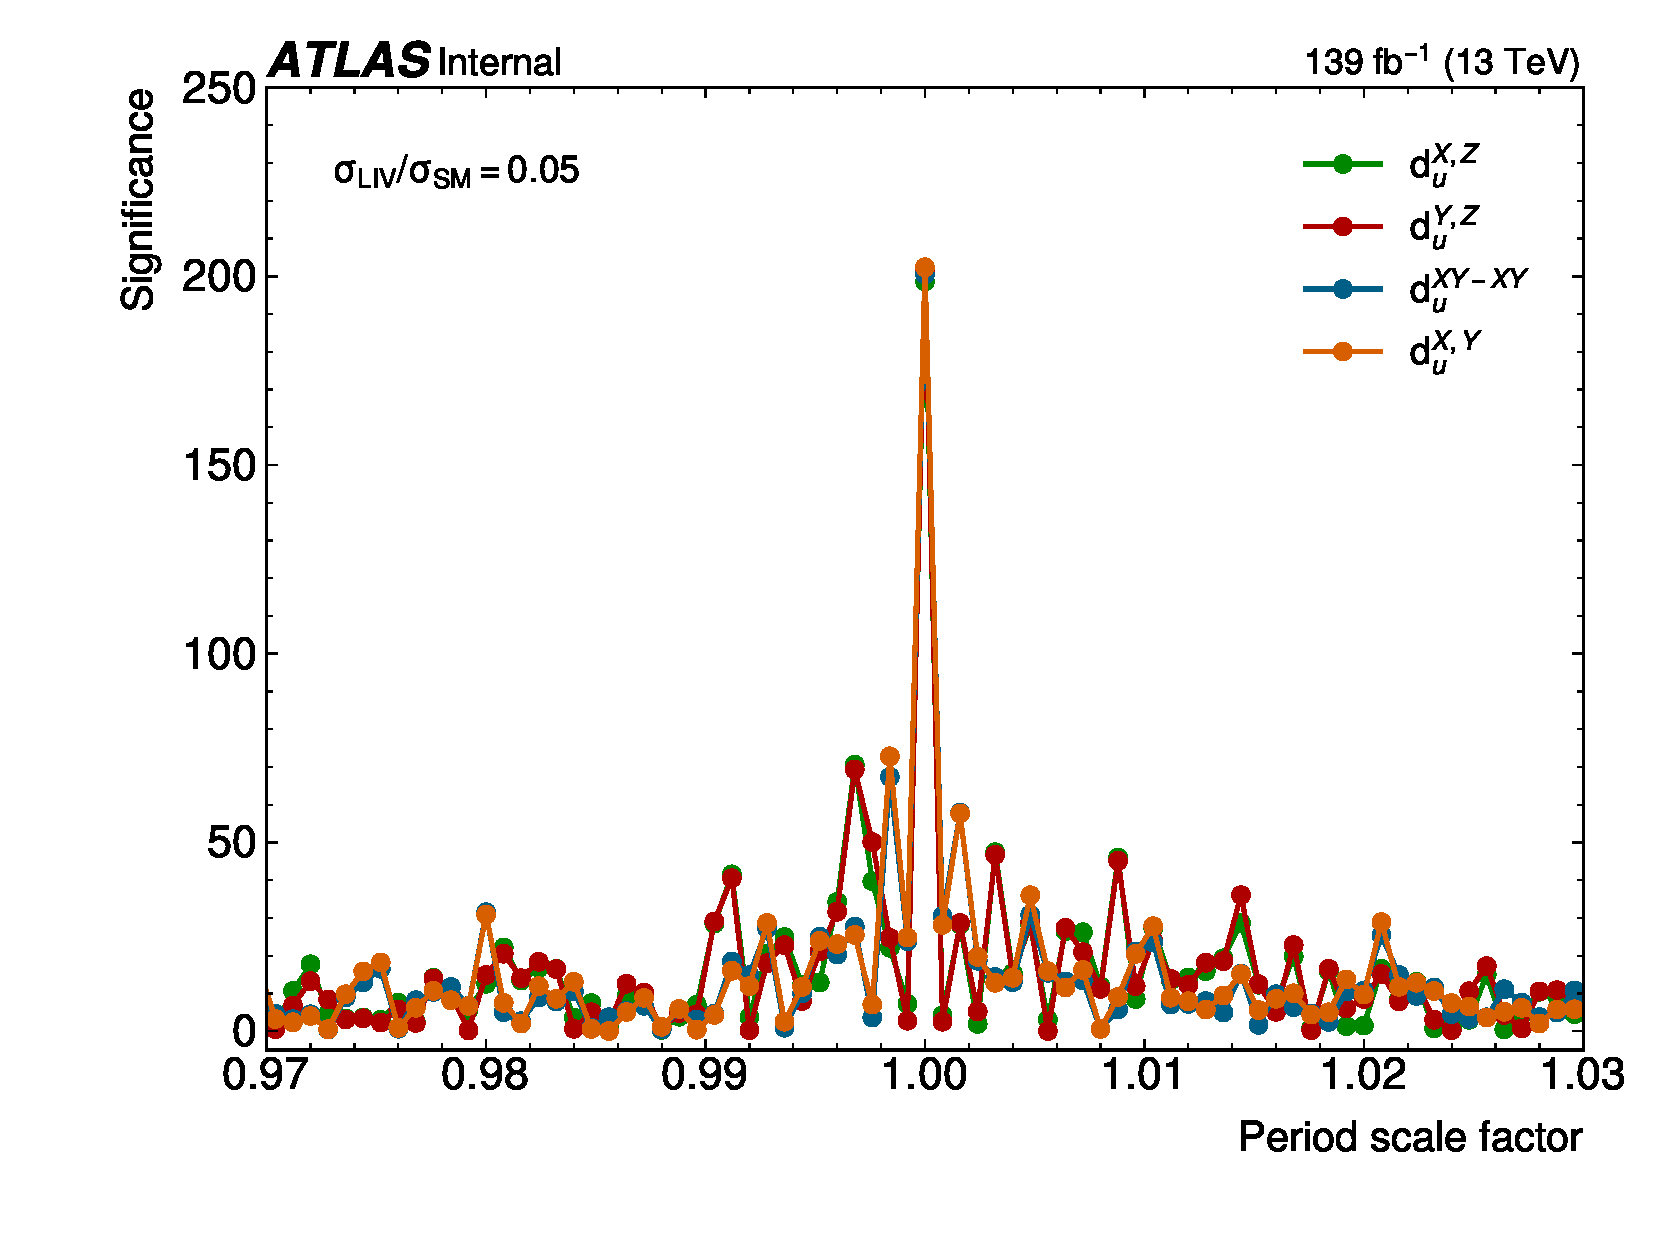
\includegraphics[width=0.6\textwidth]{figs/toy/sig_periodscale_zoom.pdf}
\caption{\label{fig:toy_sig_periodscale_zoom} Significance (quadrature sum of deviataion from 1 on the double ratio in sidereal 100 bins) as function of 
probing period scale factor with no random case. Injected LIV amplitude is 1 pb.  The period with scale factor = 1 is the 23h56m04s, which is used to generate signal.  { TO BE UPDATED with figure from Ablet} }
\end{figure}


\begin{figure}
\centering
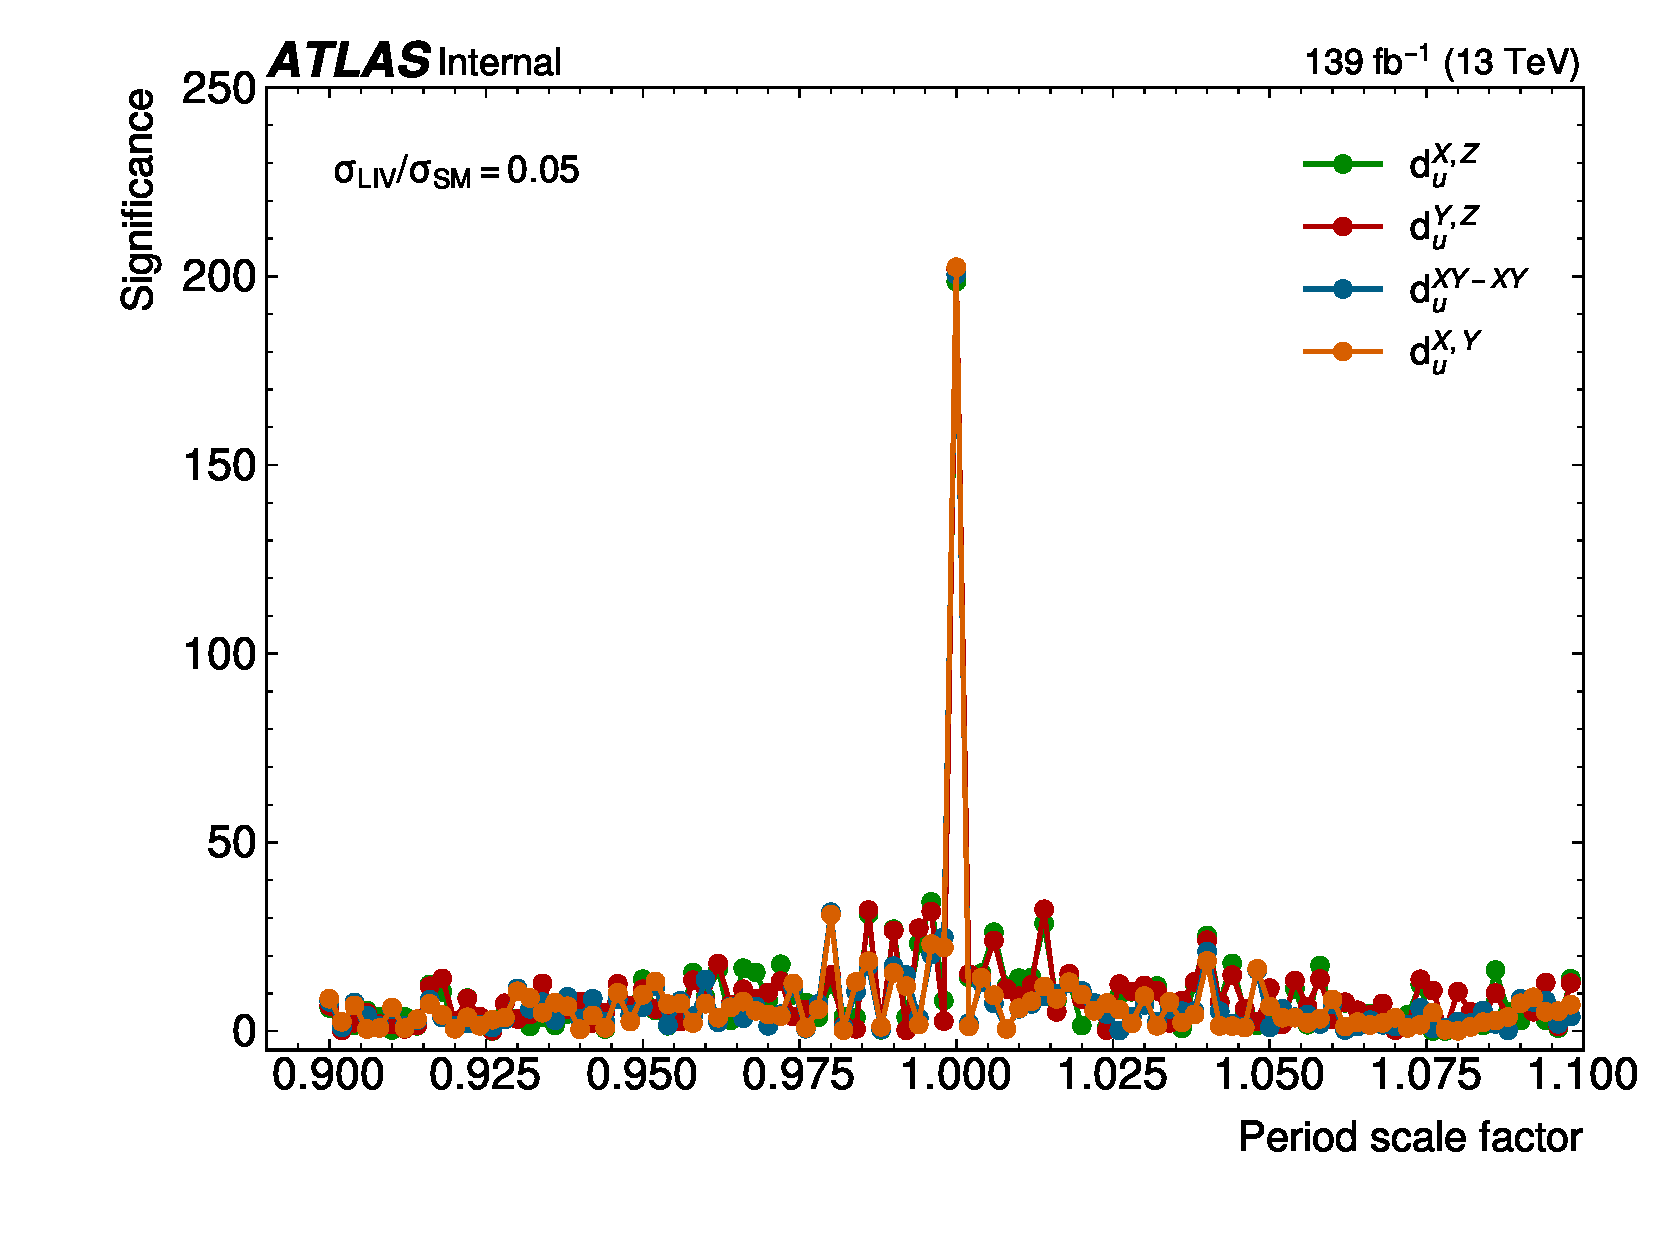
\includegraphics[width=0.6\textwidth]{figs/toy/sig_periodscale2.pdf}
\caption{\label{fig:toy_sig_periodscale} Significance as function of probing period scale factor with no random case. Injected LIV amplitude is 1 pb.  
The period with scale factor = 1 is the 23h56m04s, which is used to generate siganl. { TO BE UPDATED with figure from Ablet}}
\end{figure}
%% \subsubsection{blind TOY study}


\subsubsection{Study on the effect of correction}

 Effect of efficieincy correction is checked also simple TOY study.
Above studies are all not taken into account efficiency effect on the Z counting method. As described in Section~\ref{lab:Methodology},
there are $<\mu>$ dependent efficiency changes, i.e. on lepton reconstruction and trigger. These effects are modeled in Toy generation.
Electron efficiency is parameterized as a function of $<mu>$, and generated Toy based on it. 
Figure~\ref{fig:toy_effect_efficiency}(left) shows the double ratio with NULL signal configuration without applying the efficiency effect. 
The double ratio shows a flat dependence. Once efficiency effect taken into accout as the middle figure of Fig.~\ref{fig:toy_effect_efficiency}, 
structure showing up. This is because profile of $<mu>$ as function of sidereal phase is not flat due to limited statistics. 
This is small effect, but it become large effect on the double ratio. 

 Figure ~\ref{fig:toy_effect_efficiency}(right) shows same one after applying efficiency correction. In case the modeling of efficiency dependence is well understood,
we can minimize the modulation due to $<mu>$ dependent modulation on the double ratio. 
This could be the largest systematic uncertainty of the search.

\begin{figure}
\centering
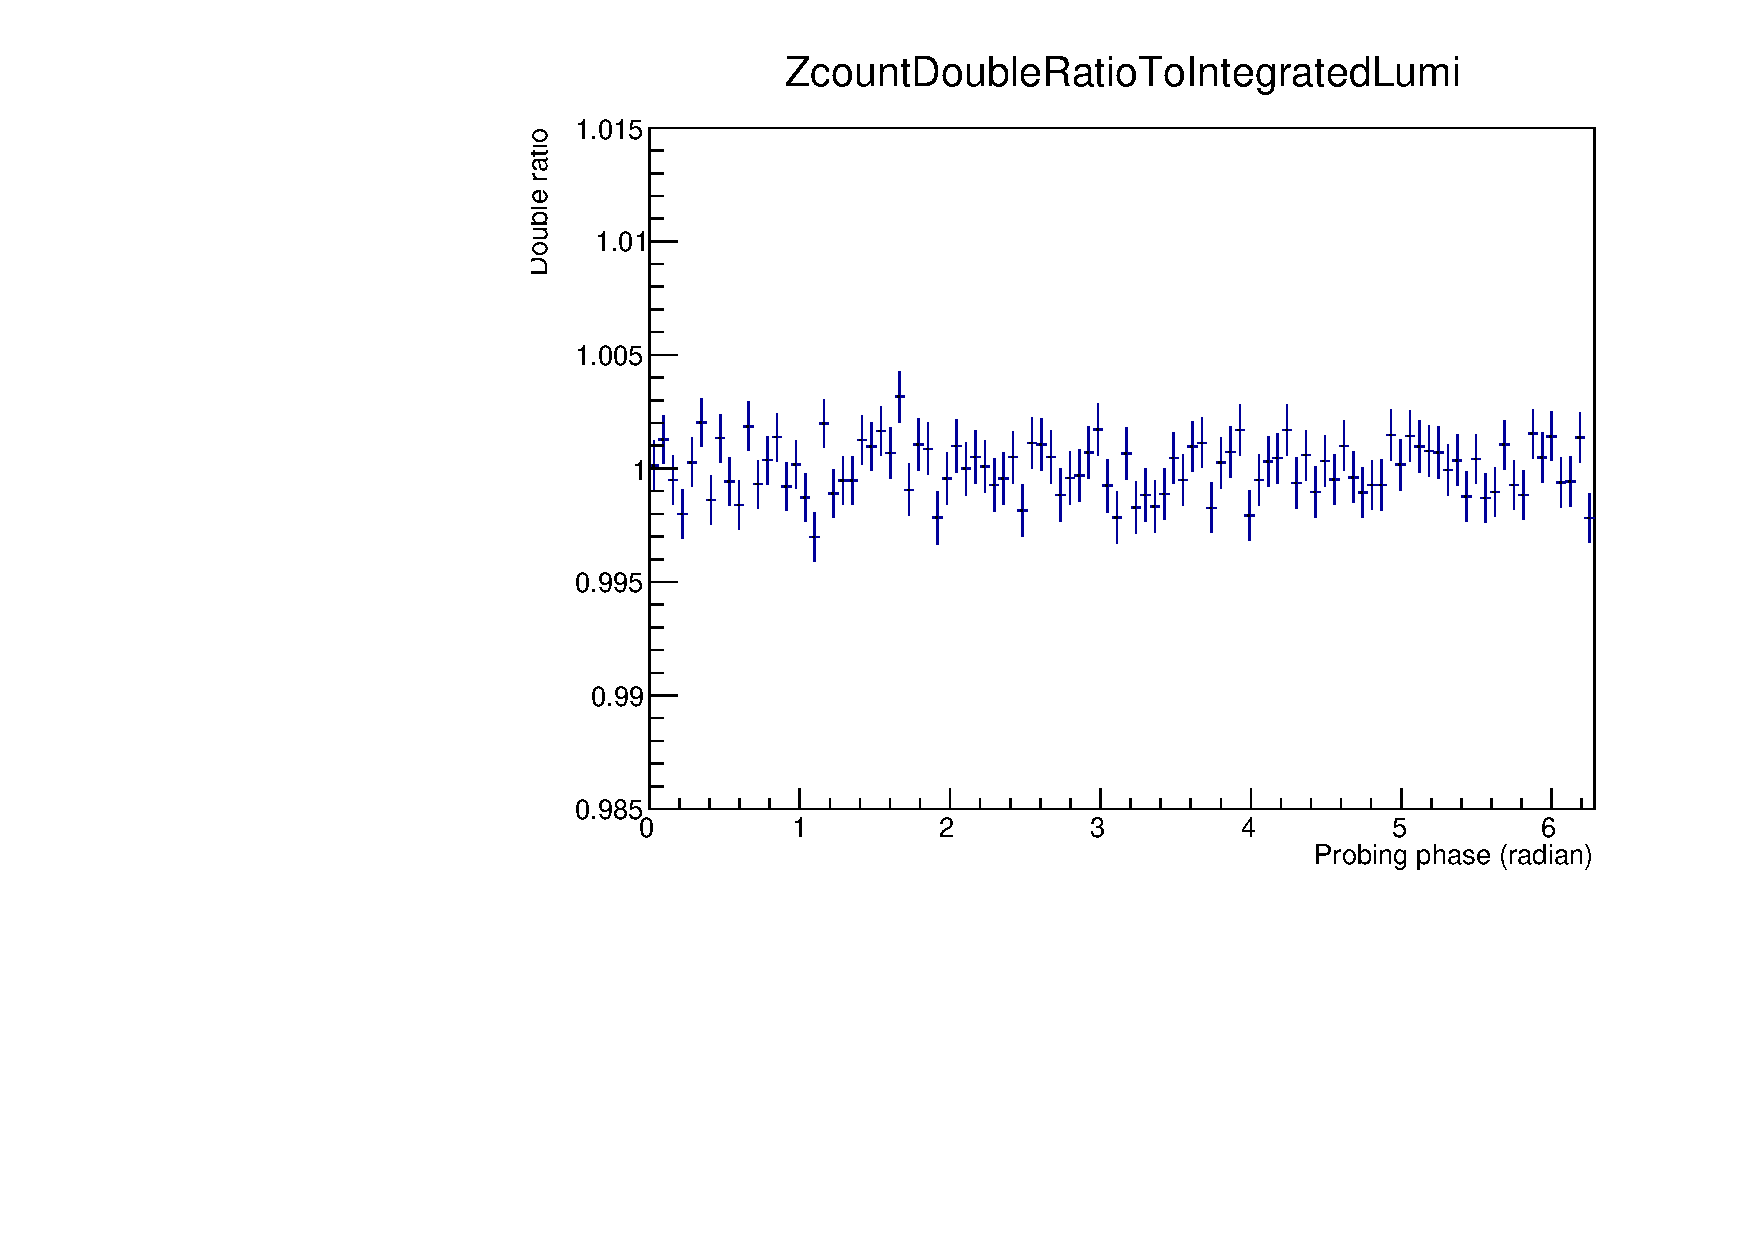
\includegraphics[width=0.33\textwidth]{figs/toy/fig_bin100_LIVxsec_0_random1_period1000_probe24_SigConfig0_LumiProf1_full_ZcountDoubleRatioToIntegratedLumi.pdf}
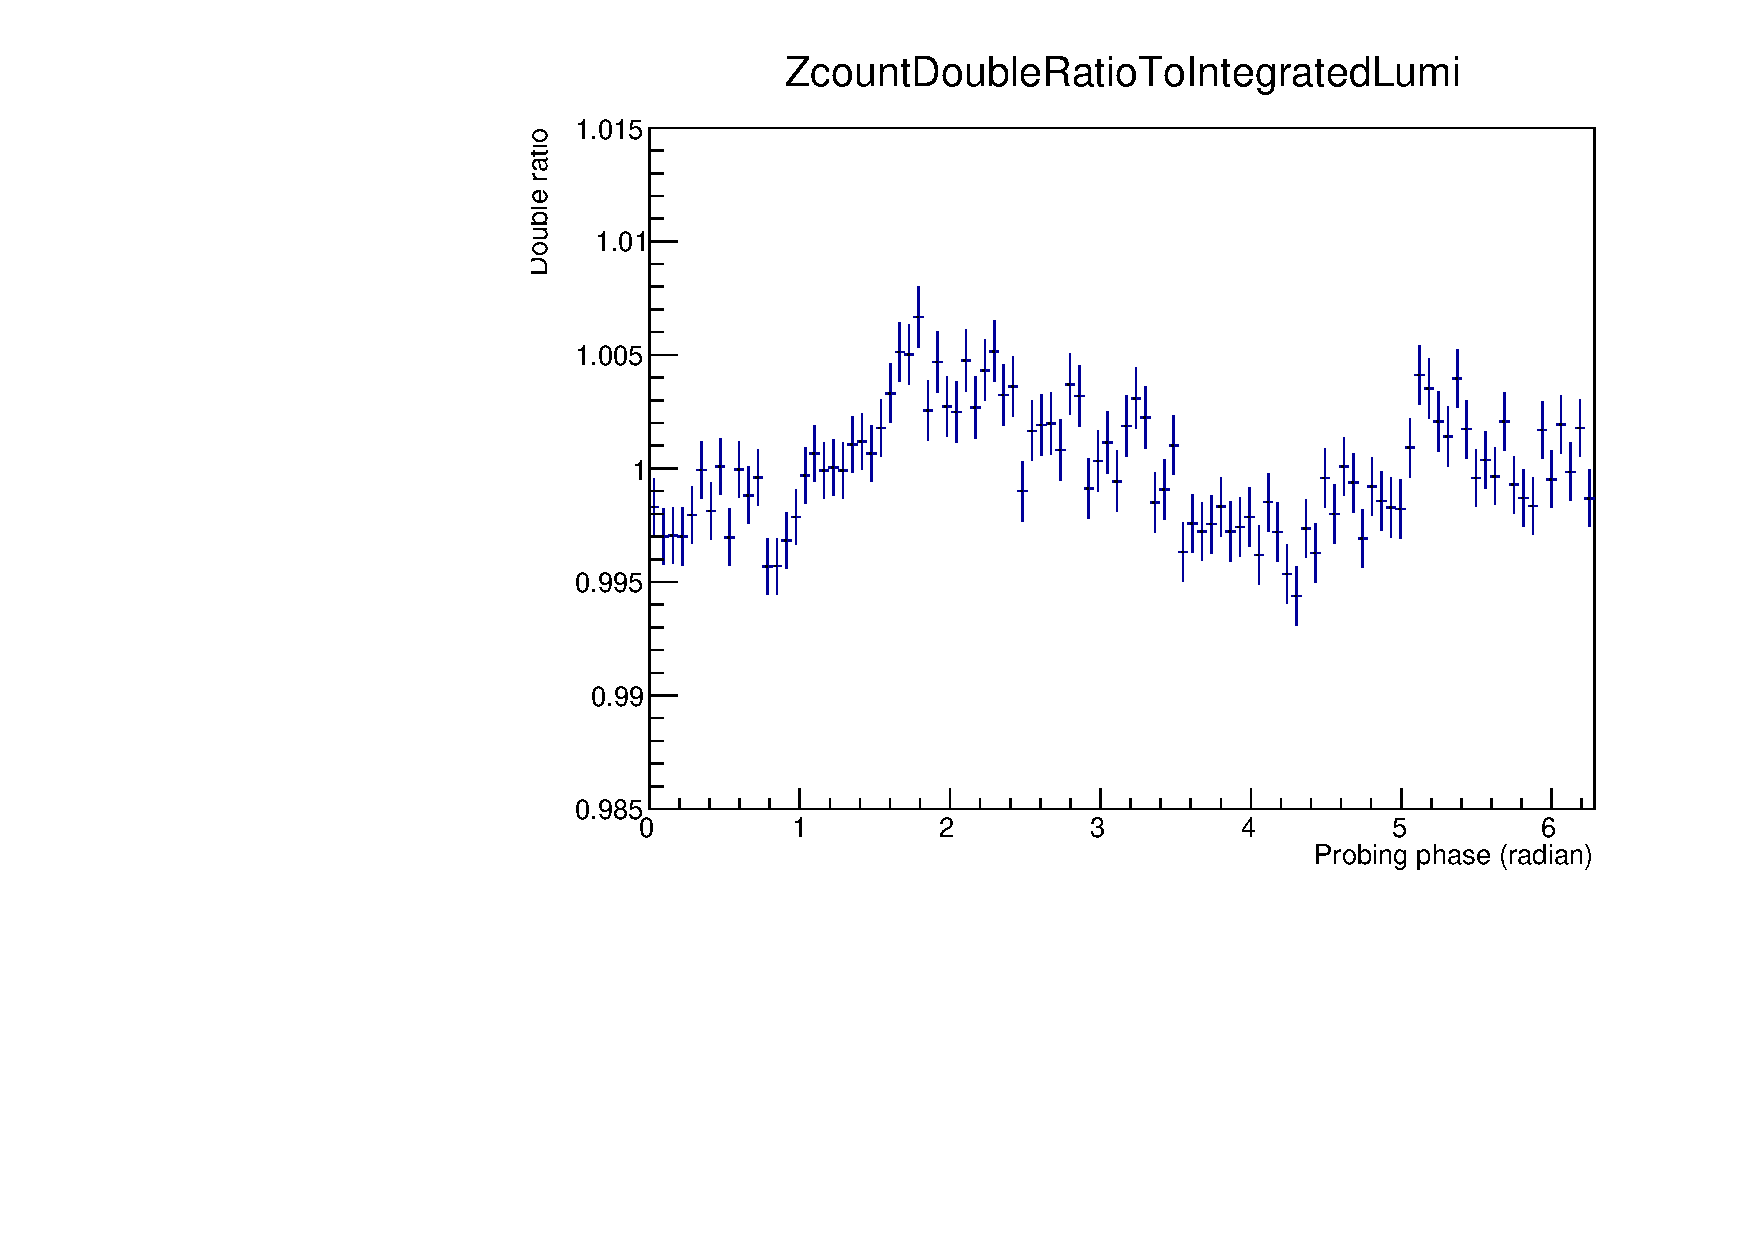
\includegraphics[width=0.33\textwidth]{figs/toy/fig_bin100_LIVxsec_0_random1_period1000_probe24_SigConfig101_LumiProf1_full_ZcountDoubleRatioToIntegratedLumi.pdf}
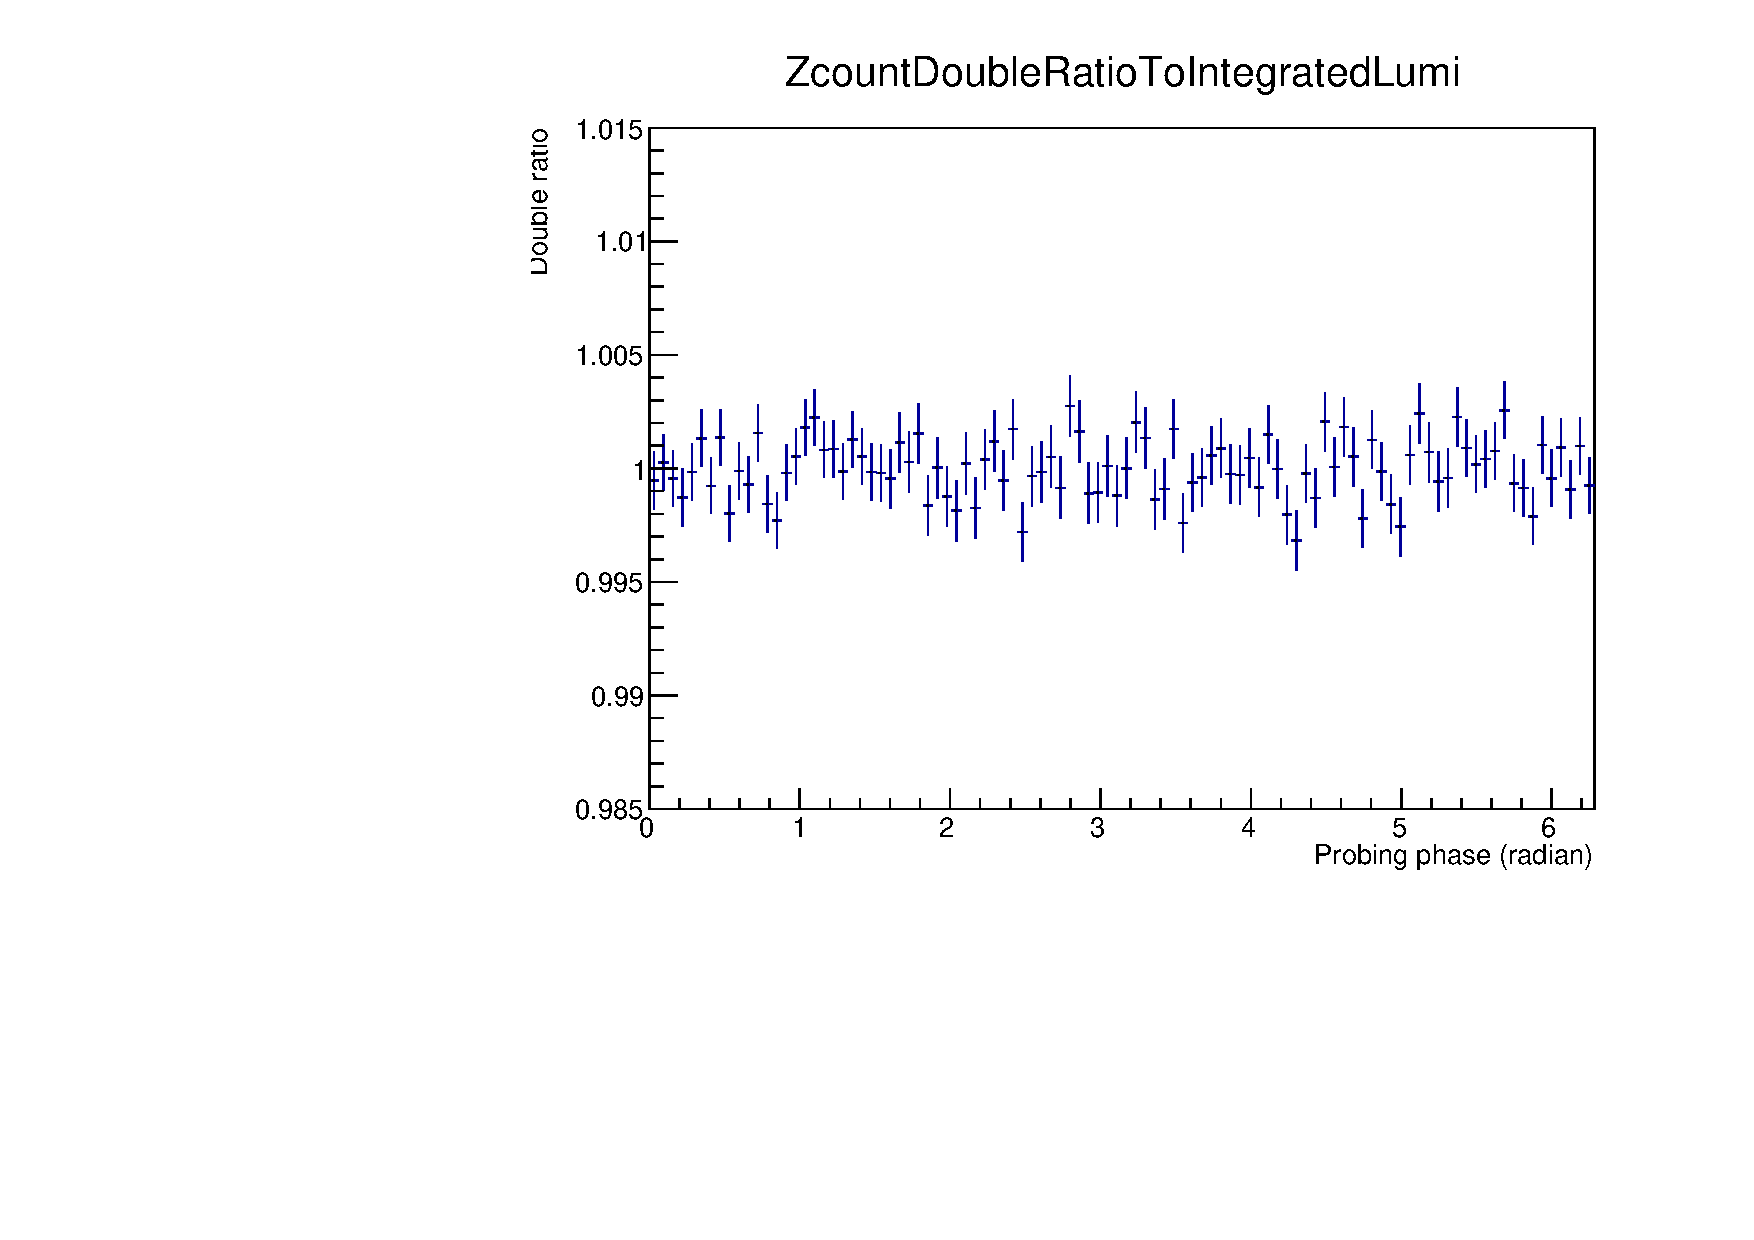
\includegraphics[width=0.33\textwidth]{figs/toy/fig_bin100_LIVxsec_0_random1_period1000_probe24_SigConfig201_LumiProf1_full_ZcountDoubleRatioToIntegratedLumi.pdf}
\caption{\label{fig:toy_effect_efficiency} Effect of efficiency correction and its correction to the double ratio. Left: The double ratio in case efficiency=1, Middle: The double ratio with efficiency effect taken into account, Right: the double ratio with efficiency effect after applying its correction. These are generated with NULL signal configuration.}
\end{figure}


\subsubsection{One run behavior with TOY experiment}
 During ATLAS data taking, we are monitoring various physics observables. Number of Z is also one of observable. 
In case a large LIV effect, we would see large effect on number of Z as function of sidereal time. 
For example, Fig.~\ref{fig:toy_large_signal} shows case of $d_u^{XY} \sim 10^{-3}$, the amplitude in the double ratio would be larger than 15\%. 
This level, we would notice during data taking or data quality check. 

\begin{figure}
\centering
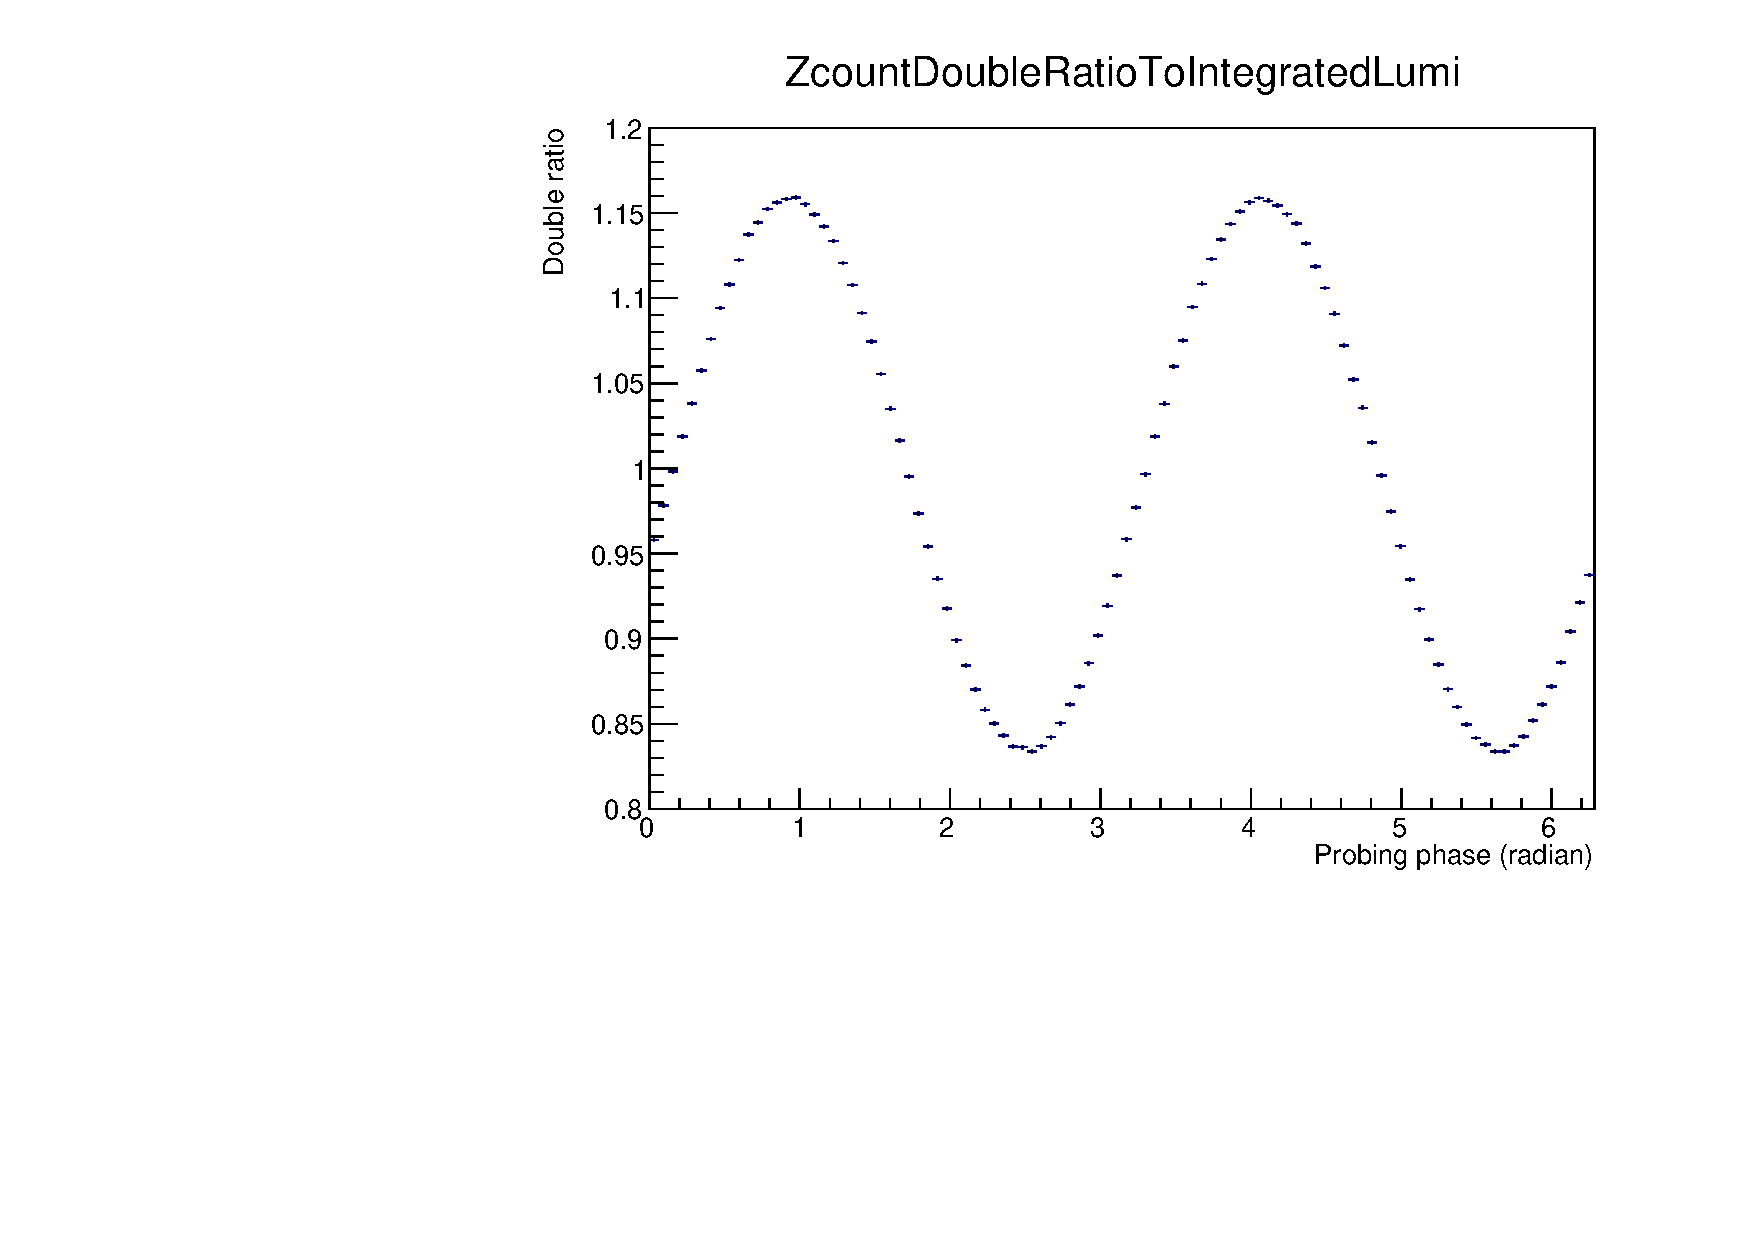
\includegraphics[width=0.4\textwidth]{figs/toy/fig_bin100_LIVxsec_577_random1_period1000_probe24_SigConfig29_LumiProf1_full_ZcountDoubleRatioToIntegratedLumi.pdf}
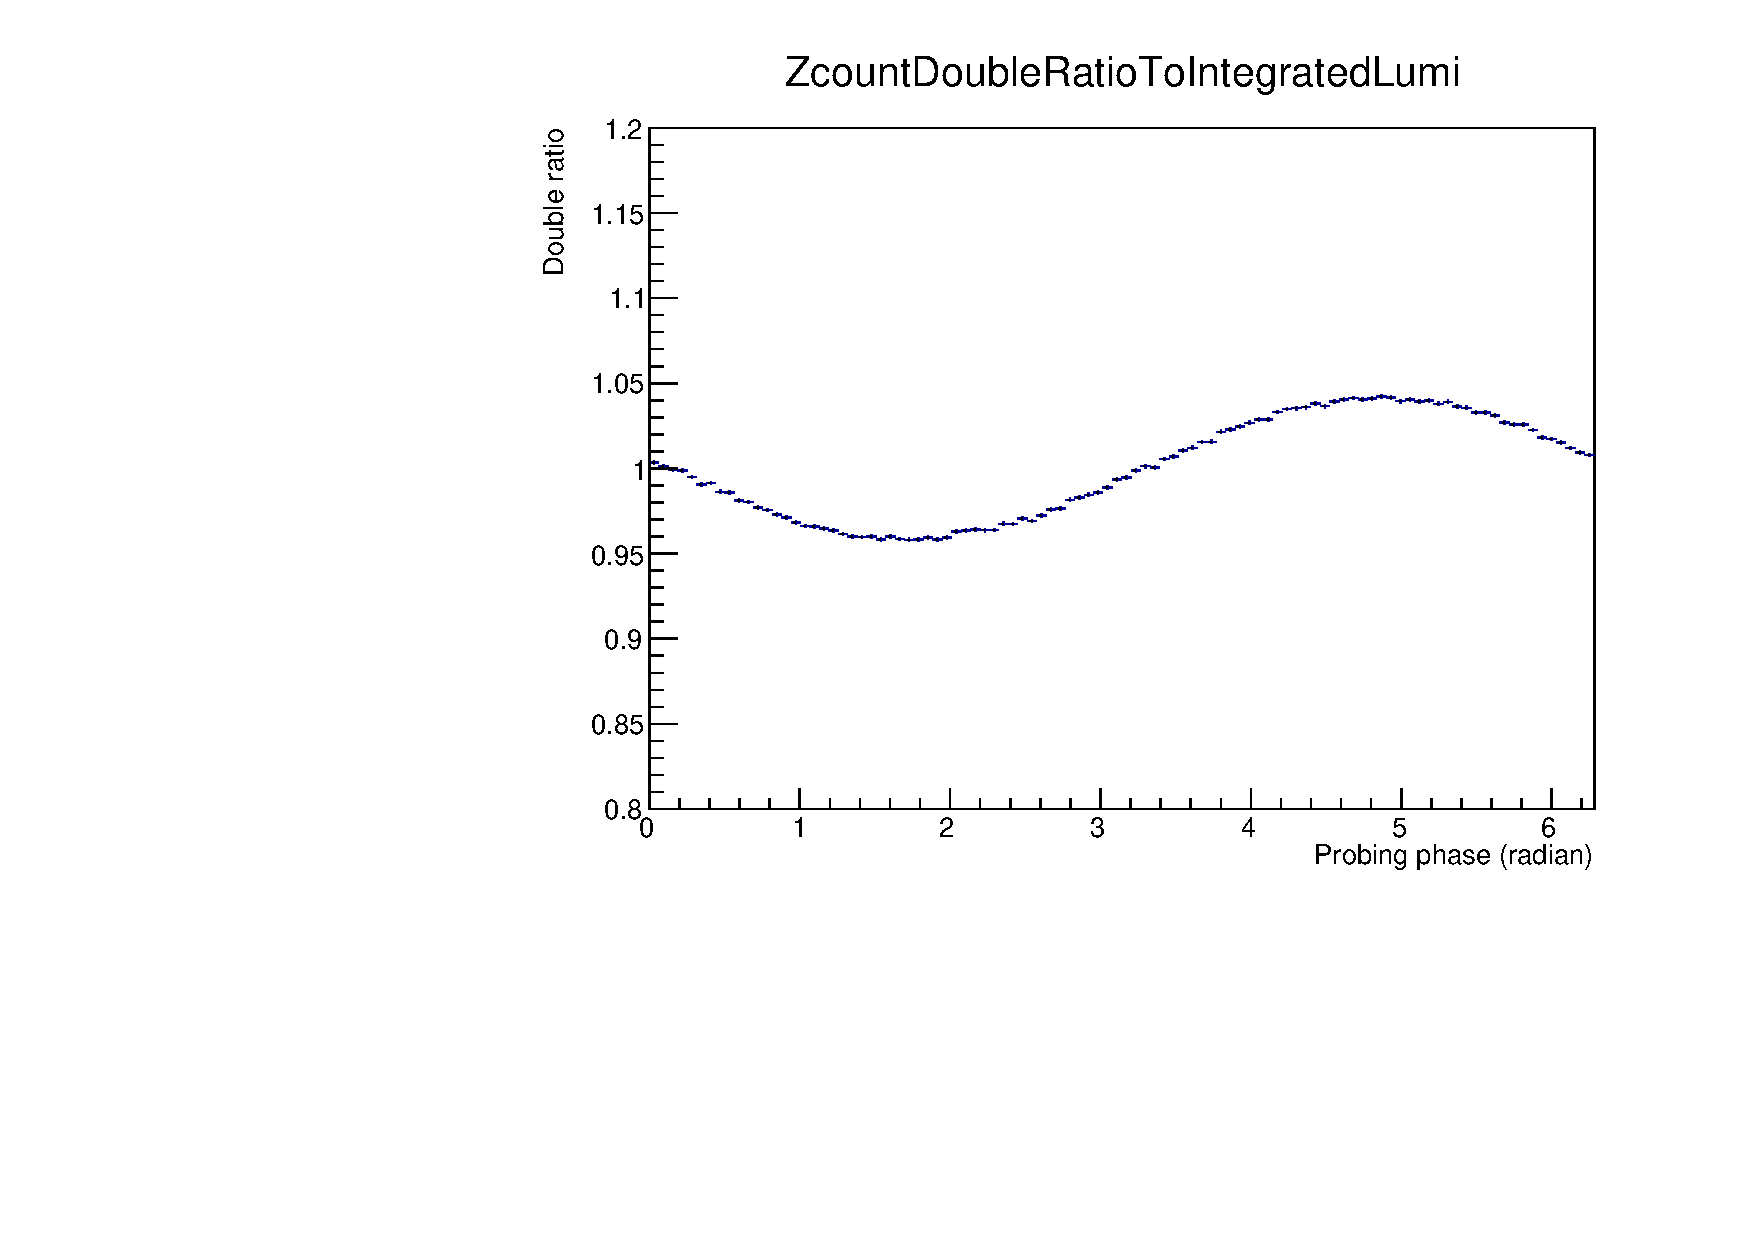
\includegraphics[width=0.4\textwidth]{figs/toy/fig_bin100_LIVxsec_577_random1_period1000_probe24_SigConfig26_LumiProf1_full_ZcountDoubleRatioToIntegratedLumi.pdf}
\caption{\label{fig:toy_large_sig_run340030} Expected double ration for the case of $d_u^{XY} = 10^{-3}$ (left) and $d_u^{YZ} = 10^{-3}$ (right). Very large oscillation would be observed.}
\end{figure}

Figure~\ref{fig:toy_large_sig_run340030} shows the expected double ratio with $d_u^{YZ} = 10^{-3}$ in the longest run in 2017 data taking. With this level of signal, 
just one run of data would be enough to notice. We consider that amplitudes larger than a few \% are already excluded. 

Relation between significance and signal strength (ratio of the amplitude of LIV effect and SM Z yields) for wilson coeffiicnets shows in Fig.~\ref{fig:toy_signif_amplitude_d}.

Peak amplitude of the LIV effect, $(\sigma_{SME}-\sigma_{SM})/\sigma_{SM}$, with wilson coefficients are one are listed Table~\ref{tab:scan_range}. 
Scan ranges for each wilson coefficient are set at the peak amplitude at 5\% which are summarized in the same Table.


\begin{figure}
\centering
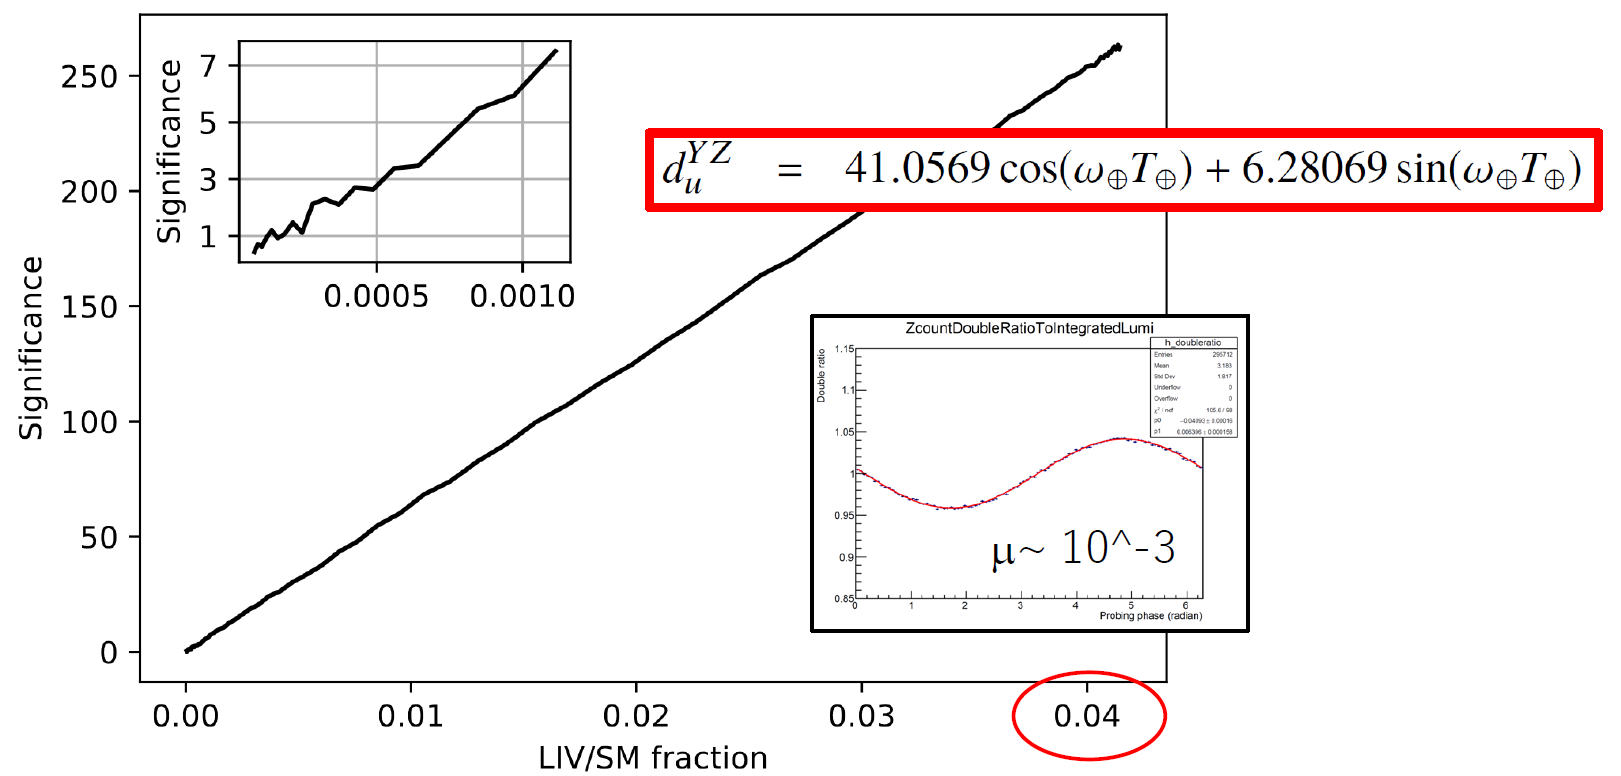
\includegraphics[width=0.43\textwidth]{figs/toy/Significance_Amplitude_for_d_YZ.png}
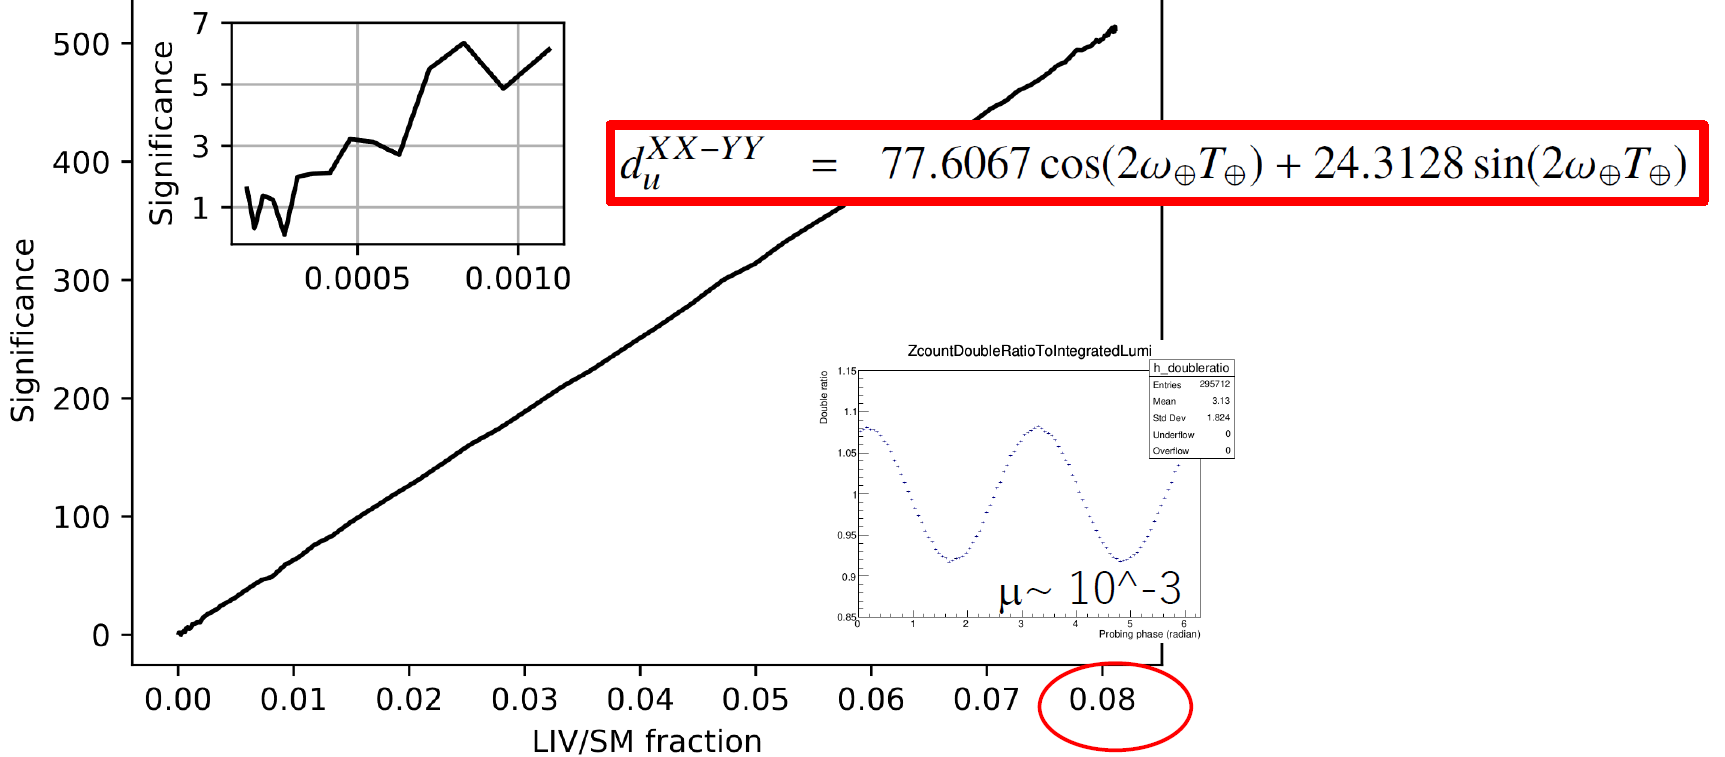
\includegraphics[width=0.46\textwidth]{figs/toy/Significance_Amplitude_for_d_XXYY.png}
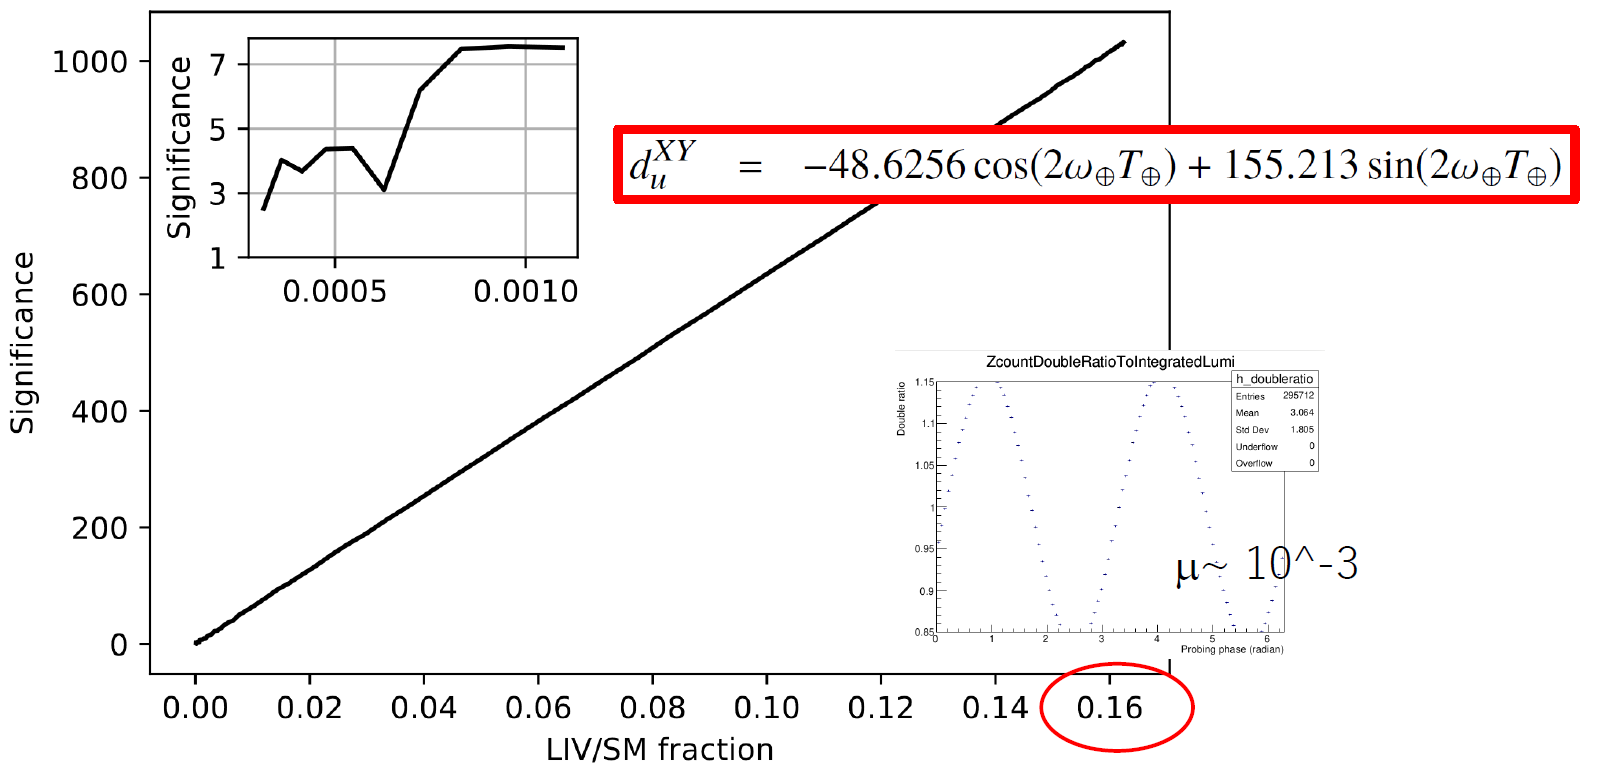
\includegraphics[width=0.43\textwidth]{figs/toy/Significance_Amplitude_for_d_XY.png}
\caption{\label{fig:toy_signif_amplitude_d} Significance as function of signal strangth for wilson coefficients $d_u^{YZ}$ (left), $d_u^{XX-YY}$ (middle) and $d_u^{XY}$ (right).}
\end{figure}



\begin{table}
\centering 
\begin{tabular}{c | c c} % centered columns (4 columns)
Coefficient & peak amplitude & upper bound (peak amplide of  = 0.05)  \\
\hline
%%   $d_u^{XZ}    $ & x.xx $ \times 10^{-z}$  \\
%%   $d_u^{YZ}    $ & x.xx $ \times 10^{-z}$  \\
%%   $d_u^{XX-YY} $ & x.xx $ \times 10^{-z}$  \\
%%   $d_u^{XY}    $ & x.xx $ \times 10^{-z}$  \\
%%   $c_u^{XZ}    $ & x.xx $ \times 10^{-z}$  \\
%%   $c_u^{YZ}    $ & x.xx $ \times 10^{-z}$  \\
%%   $c_u^{XX-YY} $ & x.xx $ \times 10^{-z}$  \\
%%   $c_u^{XY}    $ & x.xx $ \times 10^{-z}$  \\
%%   $c_d^{XZ}    $ & x.xx $ \times 10^{-z}$  \\
%%   $c_d^{YZ}    $ & x.xx $ \times 10^{-z}$  \\
%%   $c_d^{XX-YY} $ & x.xx $ \times 10^{-z}$  \\
%%   $c_d^{XY}    $ & x.xx $ \times 10^{-z}$  \\

 $d_u^{XZ}    $ & 41.53449  & 1.203819 $ \times 10^{-3}$ \\
 $d_u^{YZ}    $ & 41.53449  & 1.203819 $ \times 10^{-3}$ \\
 $d_u^{XX-YY} $ & 81.32592  & 6.148103 $ \times 10^{-4}$ \\
 $d_u^{XY}    $ & 162.6518  & 3.074048 $ \times 10^{-4}$ \\
 $c_u^{XZ}    $ & 53.45986  & 9.352805 $ \times 10^{-4}$ \\
 $c_u^{YZ}    $ & 53.45986  & 9.352805 $ \times 10^{-4}$ \\
 $c_u^{XX-YY} $ & 104.6762  & 4.776644 $ \times 10^{-4}$ \\
 $c_u^{XY}    $ & 209.3524  & 2.388322 $ \times 10^{-4}$ \\
 $c_d^{XZ}    $ & 1.200602  & 4.164584 $ \times 10^{-2}$ \\
 $c_d^{YZ}    $ & 1.200602  & 4.164584 $ \times 10^{-2}$ \\
 $c_d^{XX-YY} $ & 2.350819  & 2.126917 $ \times 10^{-2}$ \\
 $c_d^{XY}    $ & 4.701638  & 1.063459 $ \times 10^{-2}$  \\
\end{tabular}
\caption{\label{tab:scan_range} Peak amplitude of the LIV effect ($(\sigma_{SME}-\sigma_{SM})/\sigma_{SM}$) at each wilson coefficinet is 1, 
and their uppper bound of the scan range which are set at the amplitude of 5\%.}
\end{table}
  
  
  
  
  
  
  
  
  
  
  
